\section{Two-Particle Correlation Function}

In this analysis with ALEPH open data, charged particles with transverse momentum between 0.1 and 4.0 GeV/$c$ 
are selected for the correlation function analysis. High multiplicity events are sampled using the total number of selected proton, 
pions and kaons (hadron multiplicity $N$) in each event. The first step in extracting the correlation function was to divide the sample 
into bins in the hadron multiplicity. For each hadron multiplicity class, ``trigger" particles are defined as charged hadrons in the selected transverse momentum range (0.1 and 4.0 GeV/$c$). Particle pairs are then formed by associating every trigger particle with the remaining charged hadrons in the same $p_{\rm T}$ interval as the trigger particle. The per-trigger-particle associated yield is defined as:
\begin{eqnarray}
\label{eq:associatedyield}
\frac{1}{N_{\rm trig}}\frac{\rm d^2N^{pair}}{d\Delta\eta  \rm d\Delta\phi}= B(0,0) \times \frac{S(\Delta\eta, \Delta\phi)}{B(\Delta\eta, \Delta\phi)}
\end{eqnarray}
where $N_{trig}$ is the number of trigger particles in the event, $\Delta\eta$ and $\Delta\phi$ are the differences in $\eta$ and $\phi$ of the pair. The signal distribution, $S(\Delta\eta, \Delta\phi)$, 
is the per-trigger-particle yield of particle pairs in the same event: 
\begin{eqnarray}
\label{eq:S}
S(\Delta\eta,\Delta\phi) = \frac{1}{N_{trig}}\frac{\rm d^2 N^{\rm same}}{\rm d\Delta\eta \rm d\Delta\phi}
\end{eqnarray}
The mixed-event background distribution, used to account for random combinatorial background, is defined as 
\begin{eqnarray}
\label{eq:B}
B(\Delta\eta,\Delta\phi) = \frac{1}{N_{trig}}\frac{\rm d^2 N^{\rm mix}}{\rm d\Delta\eta \rm d\Delta\phi}
\end{eqnarray}
and is constructing by pairing the trigger particles from two random events in the same hadron multiplicity interval.
The symbol $N^{mix}$ denotes the number of pairs taken from the mixed event, while $B(0,0)$ represents the mixed-event associated yield for both particles of the pair going in the same direction and thus having full pair acceptance. Therefore, 
the ratio $B(0,0)/B(\Delta\eta,\Delta\phi)$ represents the pair-acceptance correction factor used to derive the corrected per-trigger-particle
associated yield distribution.  The signal and background distributions are first calculated for each event and then averaged over all the events within the track multiplicity class. 

In the full data analysis, a matching between particles and the primary vertex should be performed so that the studies are done with primary hadrons from a single primary vertex. This matching requirement is not yet included in this preliminary analysis due to the limited information in the Belle open data. 



%%%%%%%%%%%%%%%%%%%%%%%%%%%%%%%%%%%%%%%%%%%%%%%%%%%%%%%%%%%%%%%% LEP1 BEAM AXIS %%%%%%%%%%%%%%%%%%%%%%%%%%%%%%%%%%%%%%%%%%%%%%%%%%%%%%%%%%%%%%%%
%%%%%%%%%%%%%%%%%%%%%%%%%%%%%%%% Multiplicity 0-20 %%%%%%%%%%%%%%%%%%%%%%%%%%%%%%%%
\begin{figure}[htbp]
  \caption{LEP1 Beam Axis, Ratio Plot, Multiplicity 0-20 (Austin, Anthony, Ratio)}
  \begin{minipage}[b]{0.32\linewidth}
    \centering
    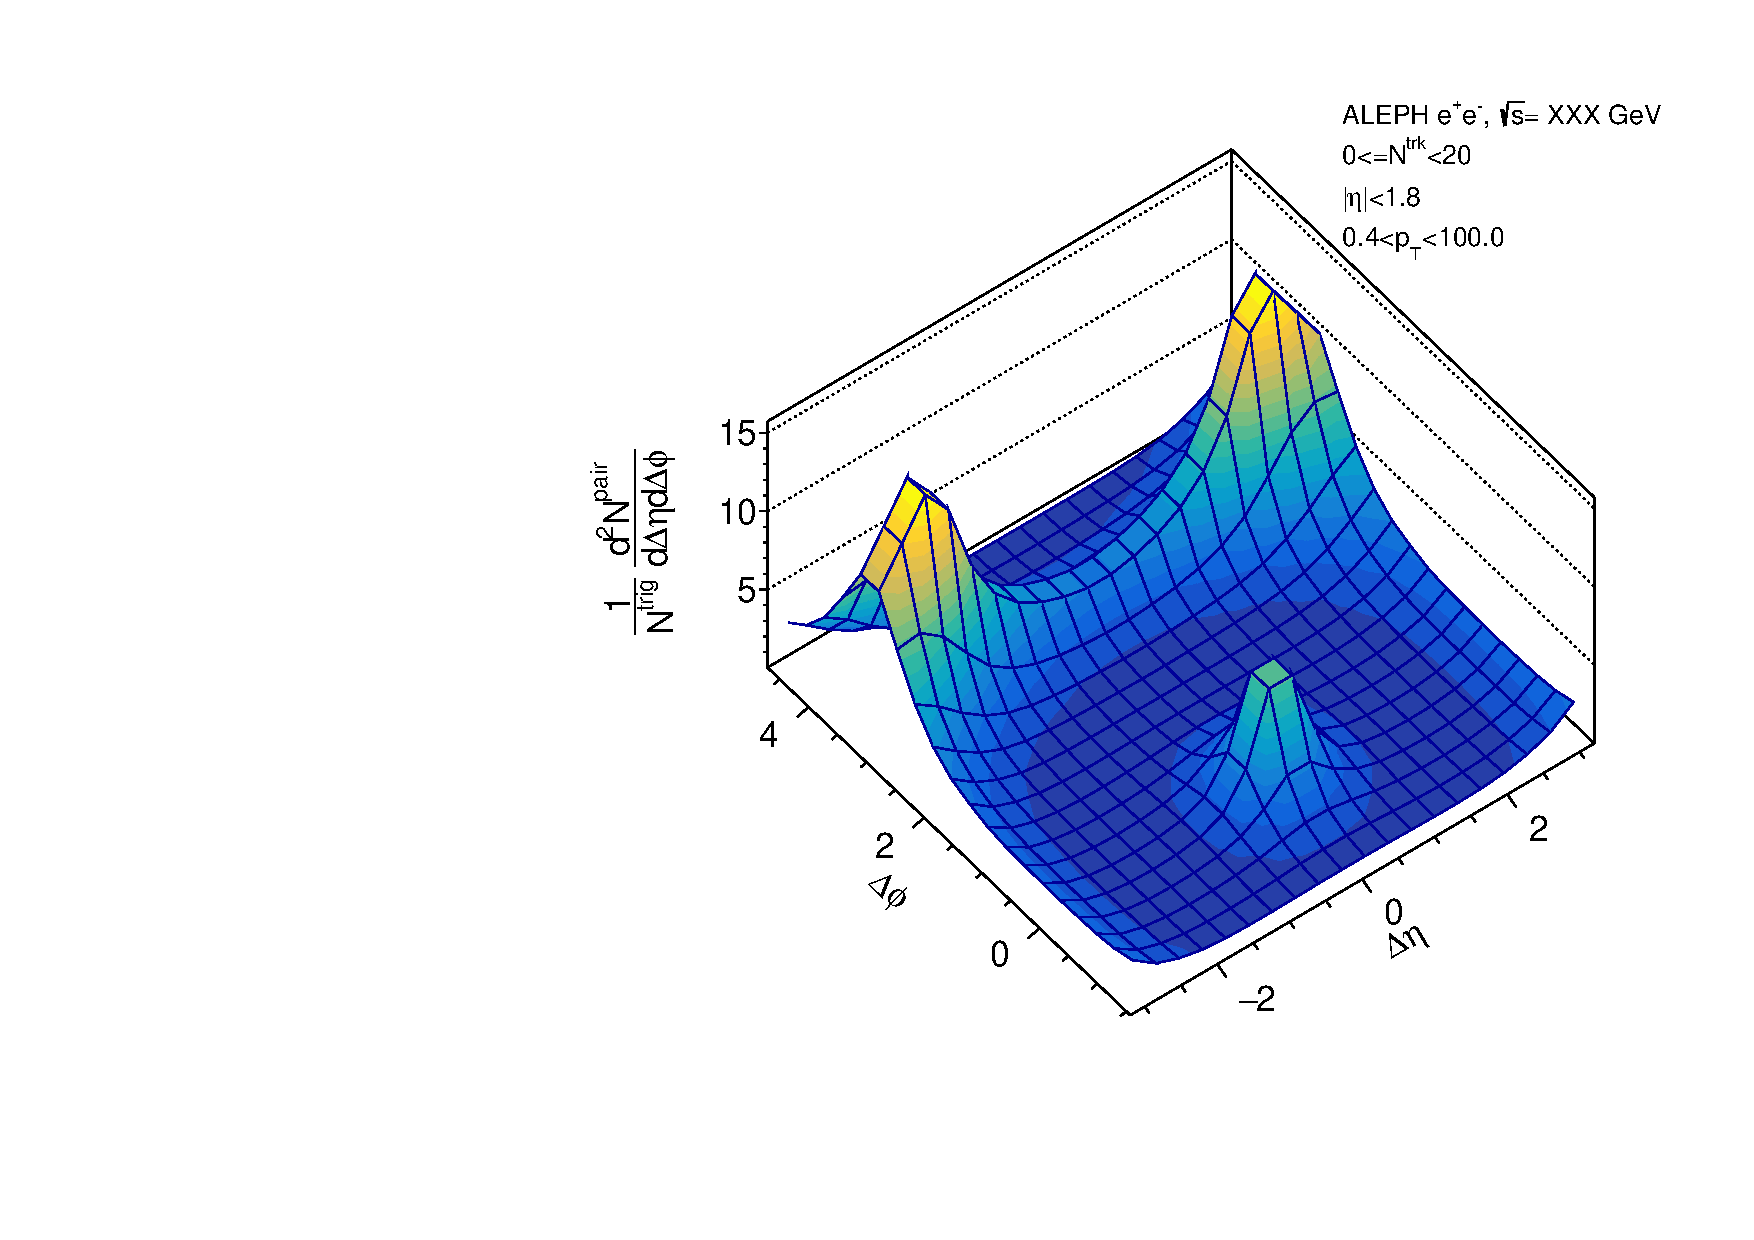
\includegraphics[width=\linewidth]{images/TwoParticleCorrelation/LEP1_BEAM/LEP1_BEAM_ratio1_0_20.pdf}
    \label{fig:LEP1 Beam Axis, Ratio Plot, Multiplicity 0-20, Austin}
  \end{minipage}
  \hspace{0.0cm}
  \begin{minipage}[b]{0.32\linewidth}
    \centering
    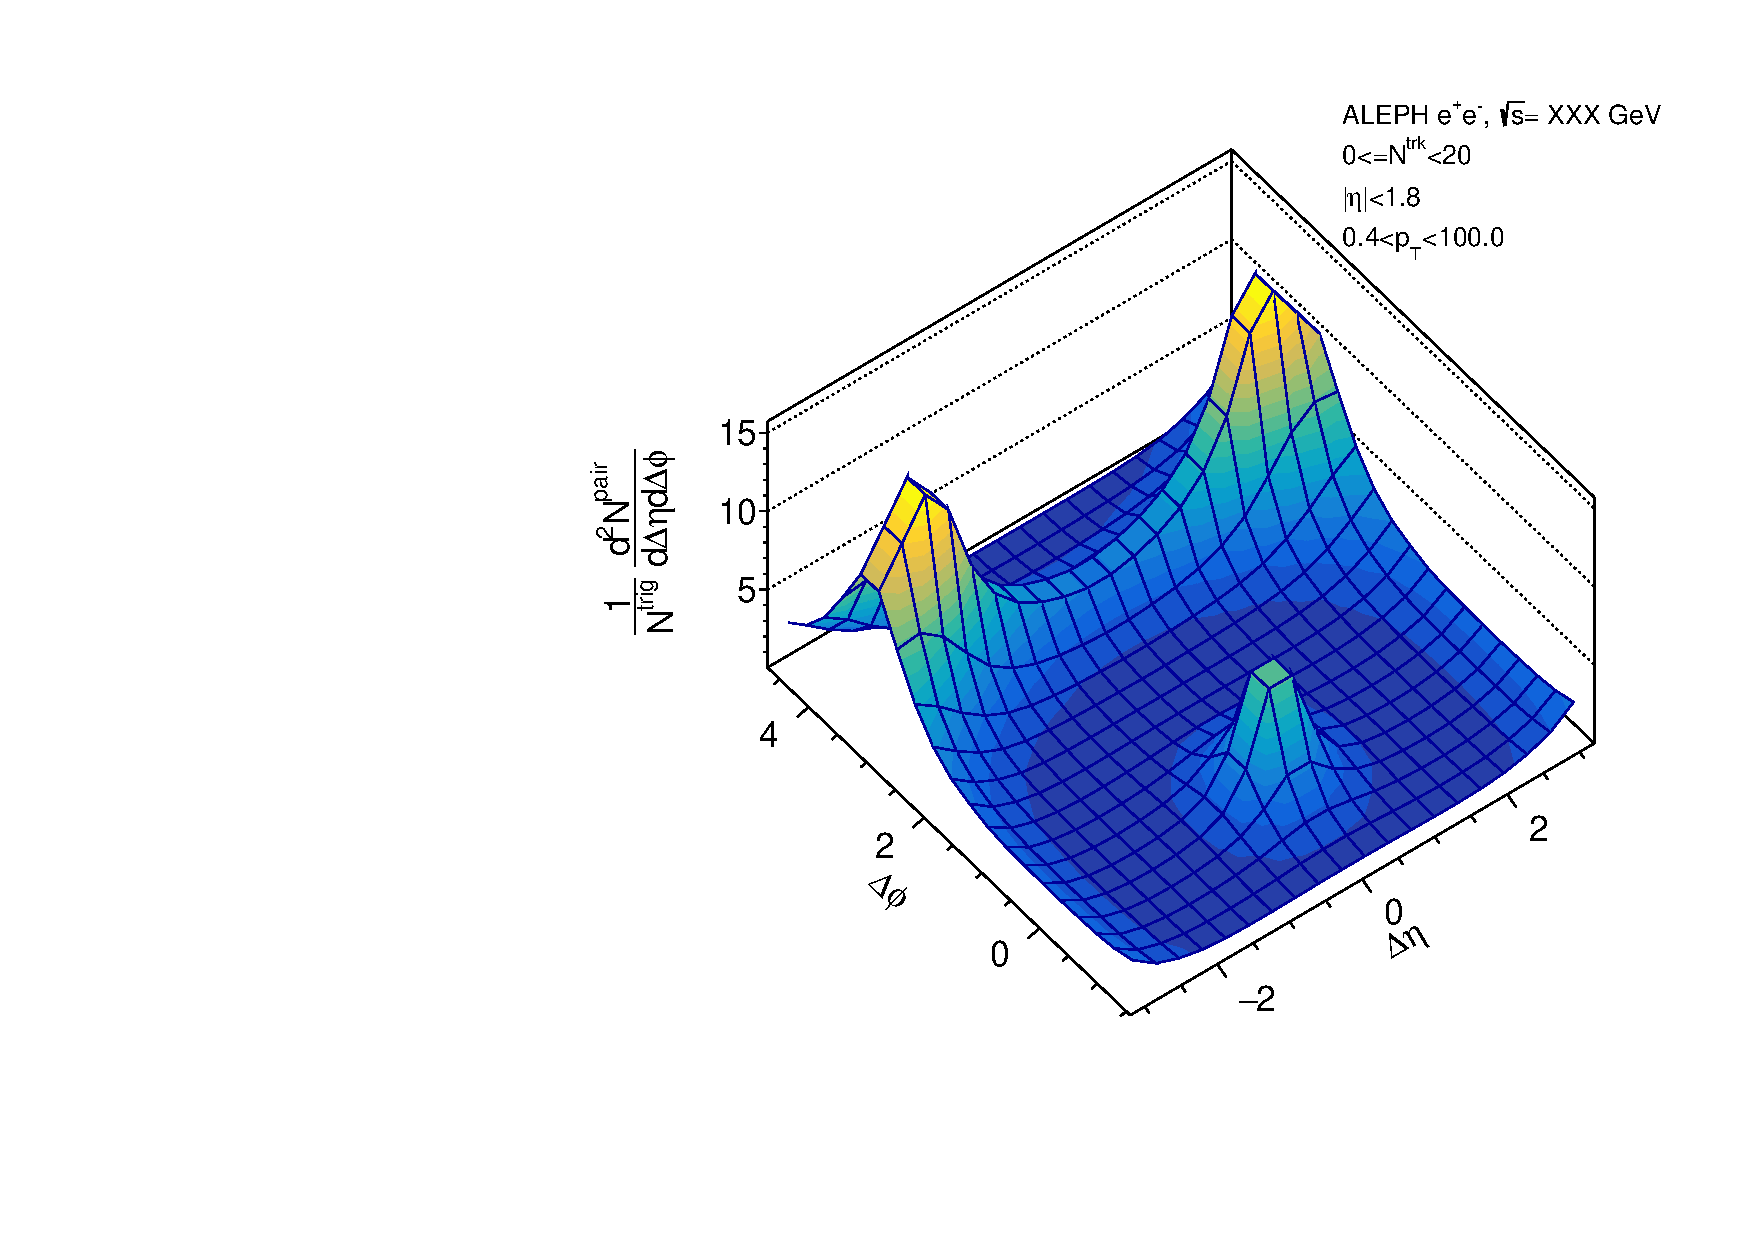
\includegraphics[width=\linewidth]{images/TwoParticleCorrelation/LEP1_BEAM/LEP1_BEAM_ratio2_0_20.pdf}
    \label{fig:LEP1 Beam Axis, Ratio Plot, Multiplicity 0-20, Anthony}
  \end{minipage}
  \hspace{0.0cm}
  \begin{minipage}[b]{0.32\linewidth}
    \centering
    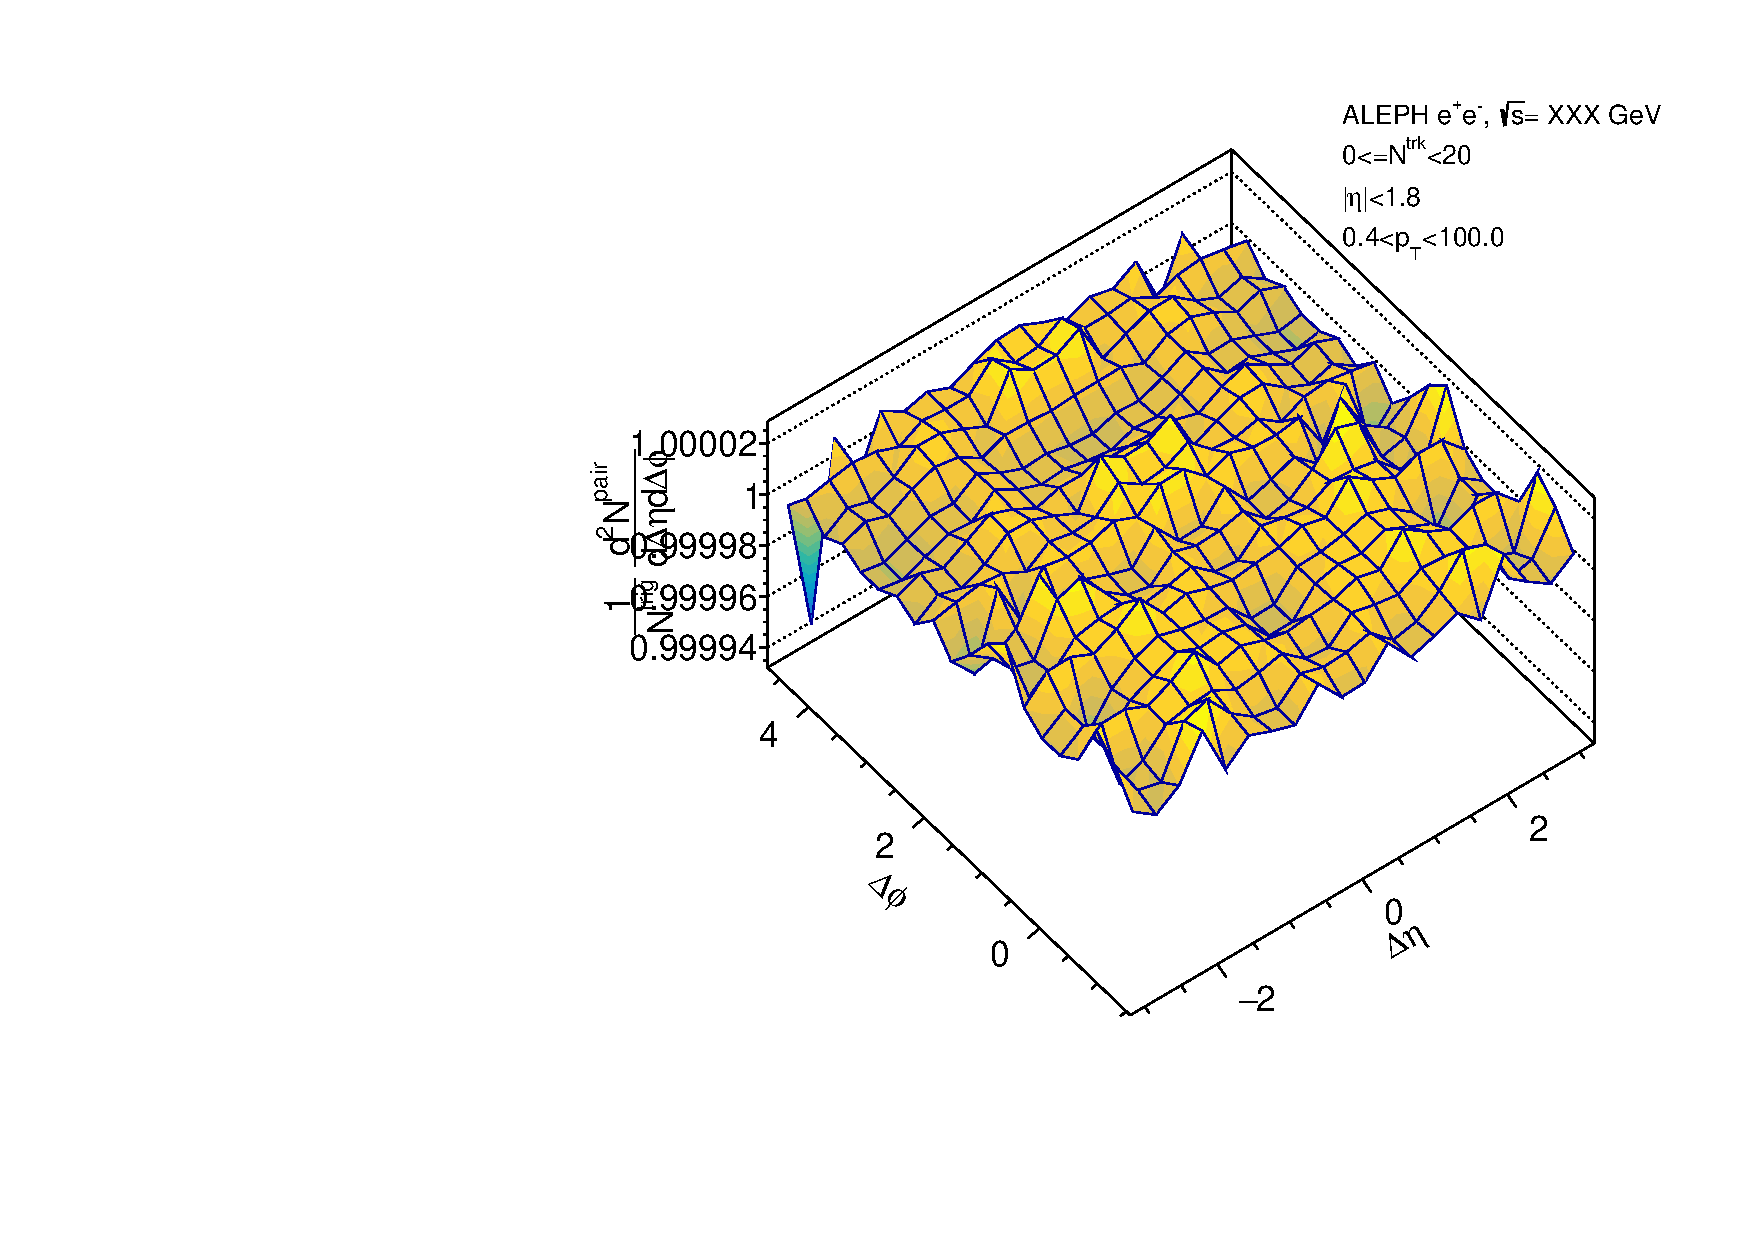
\includegraphics[width=\linewidth]{images/TwoParticleCorrelation/LEP1_BEAM/LEP1_BEAM_r_ratio_0_20.pdf}
    \label{fig:LEP1 Beam Axis, Ratio Plot, Multiplicity 0-20, Ratio}
  \end{minipage}
\end{figure}


%%%%%%%%%%%%%%%%%%%%%%%%%%%%%%%% Multiplicity 20-30 %%%%%%%%%%%%%%%%%%%%%%%%%%%%%%%%
\begin{figure}[htbp]
  \caption{LEP1 Beam Axis, Ratio Plot, Multiplicity 20-30 (Austin, Anthony, Ratio)}
  \begin{minipage}[b]{0.32\linewidth}
    \centering
    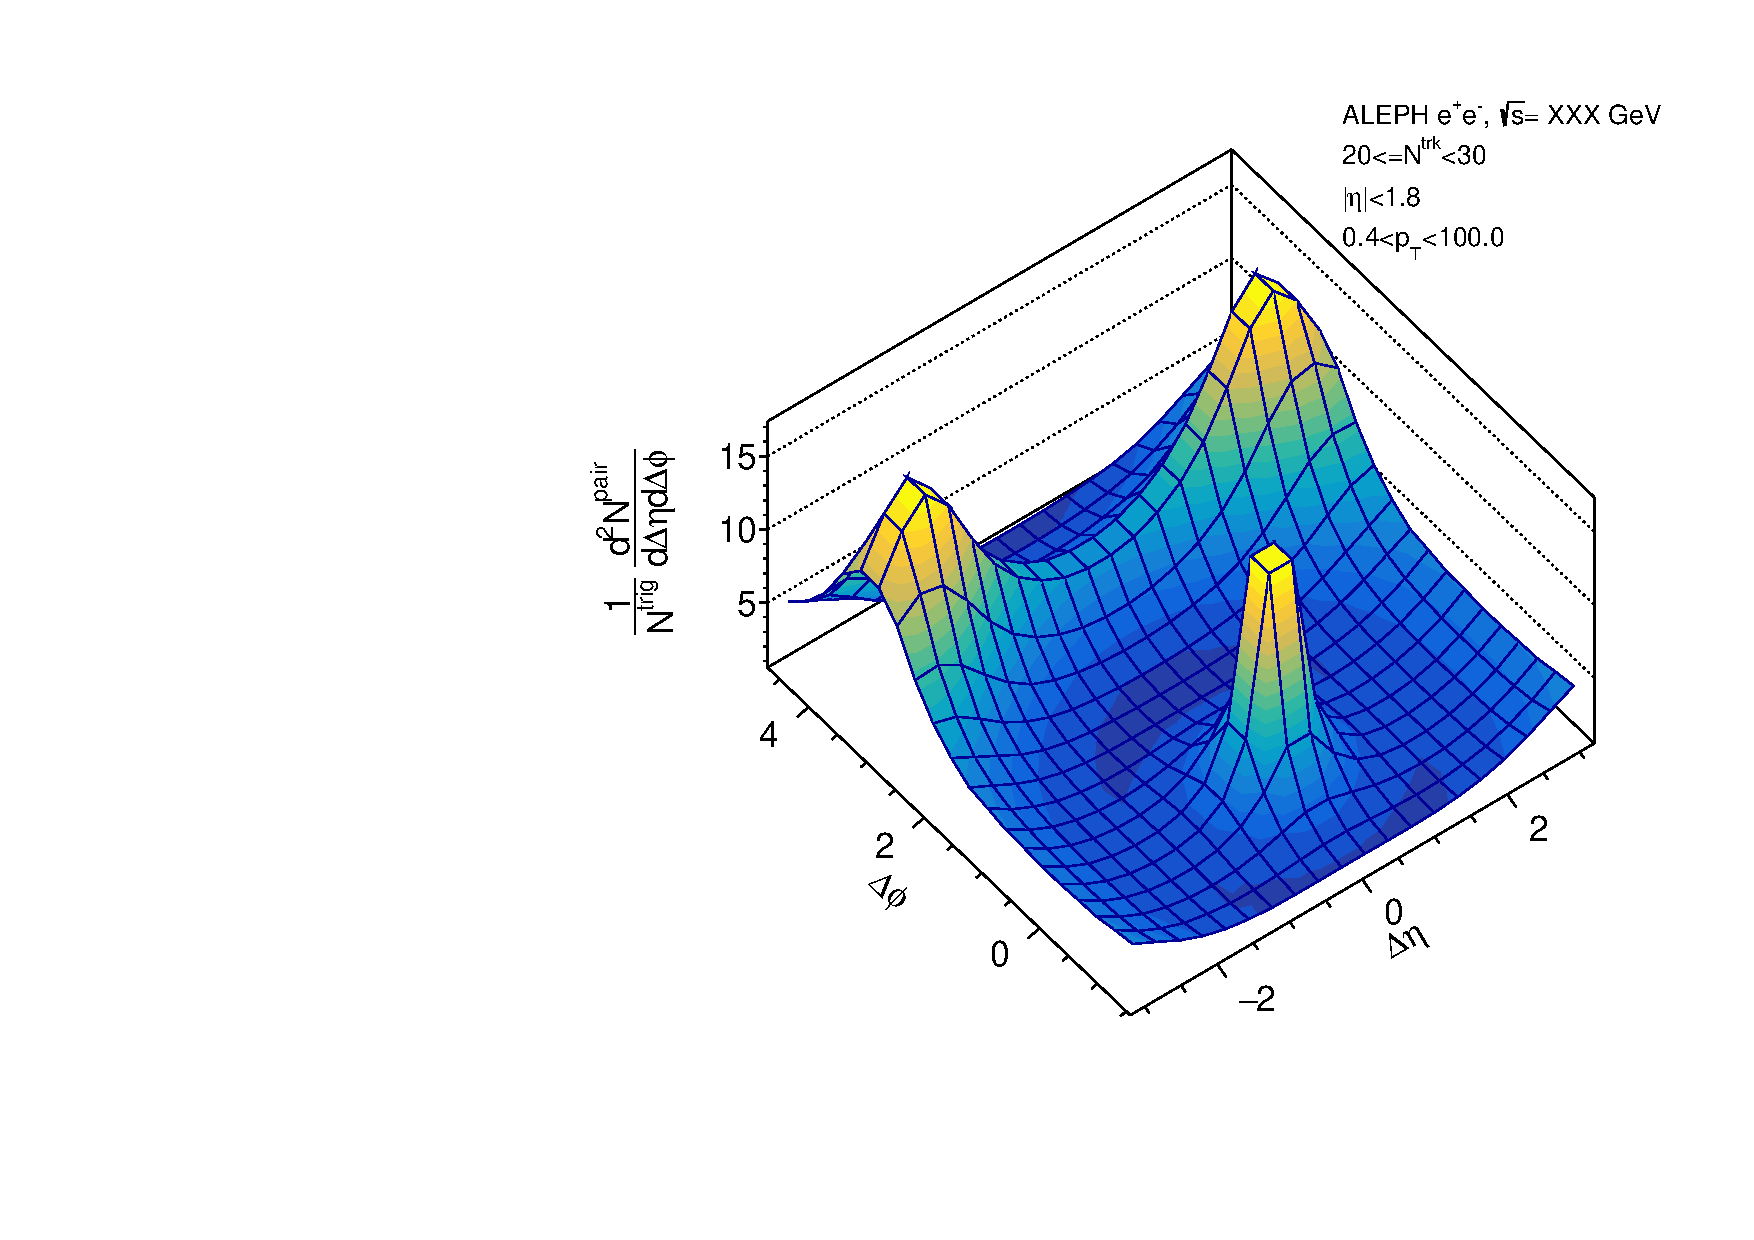
\includegraphics[width=\linewidth]{images/TwoParticleCorrelation/LEP1_BEAM/LEP1_BEAM_ratio1_20_30.pdf}
    \label{fig:LEP1 Beam Axis, Ratio Plot, Multiplicity 20-30, Austin}
  \end{minipage}
  \hspace{0.0cm}
  \begin{minipage}[b]{0.32\linewidth}
    \centering
    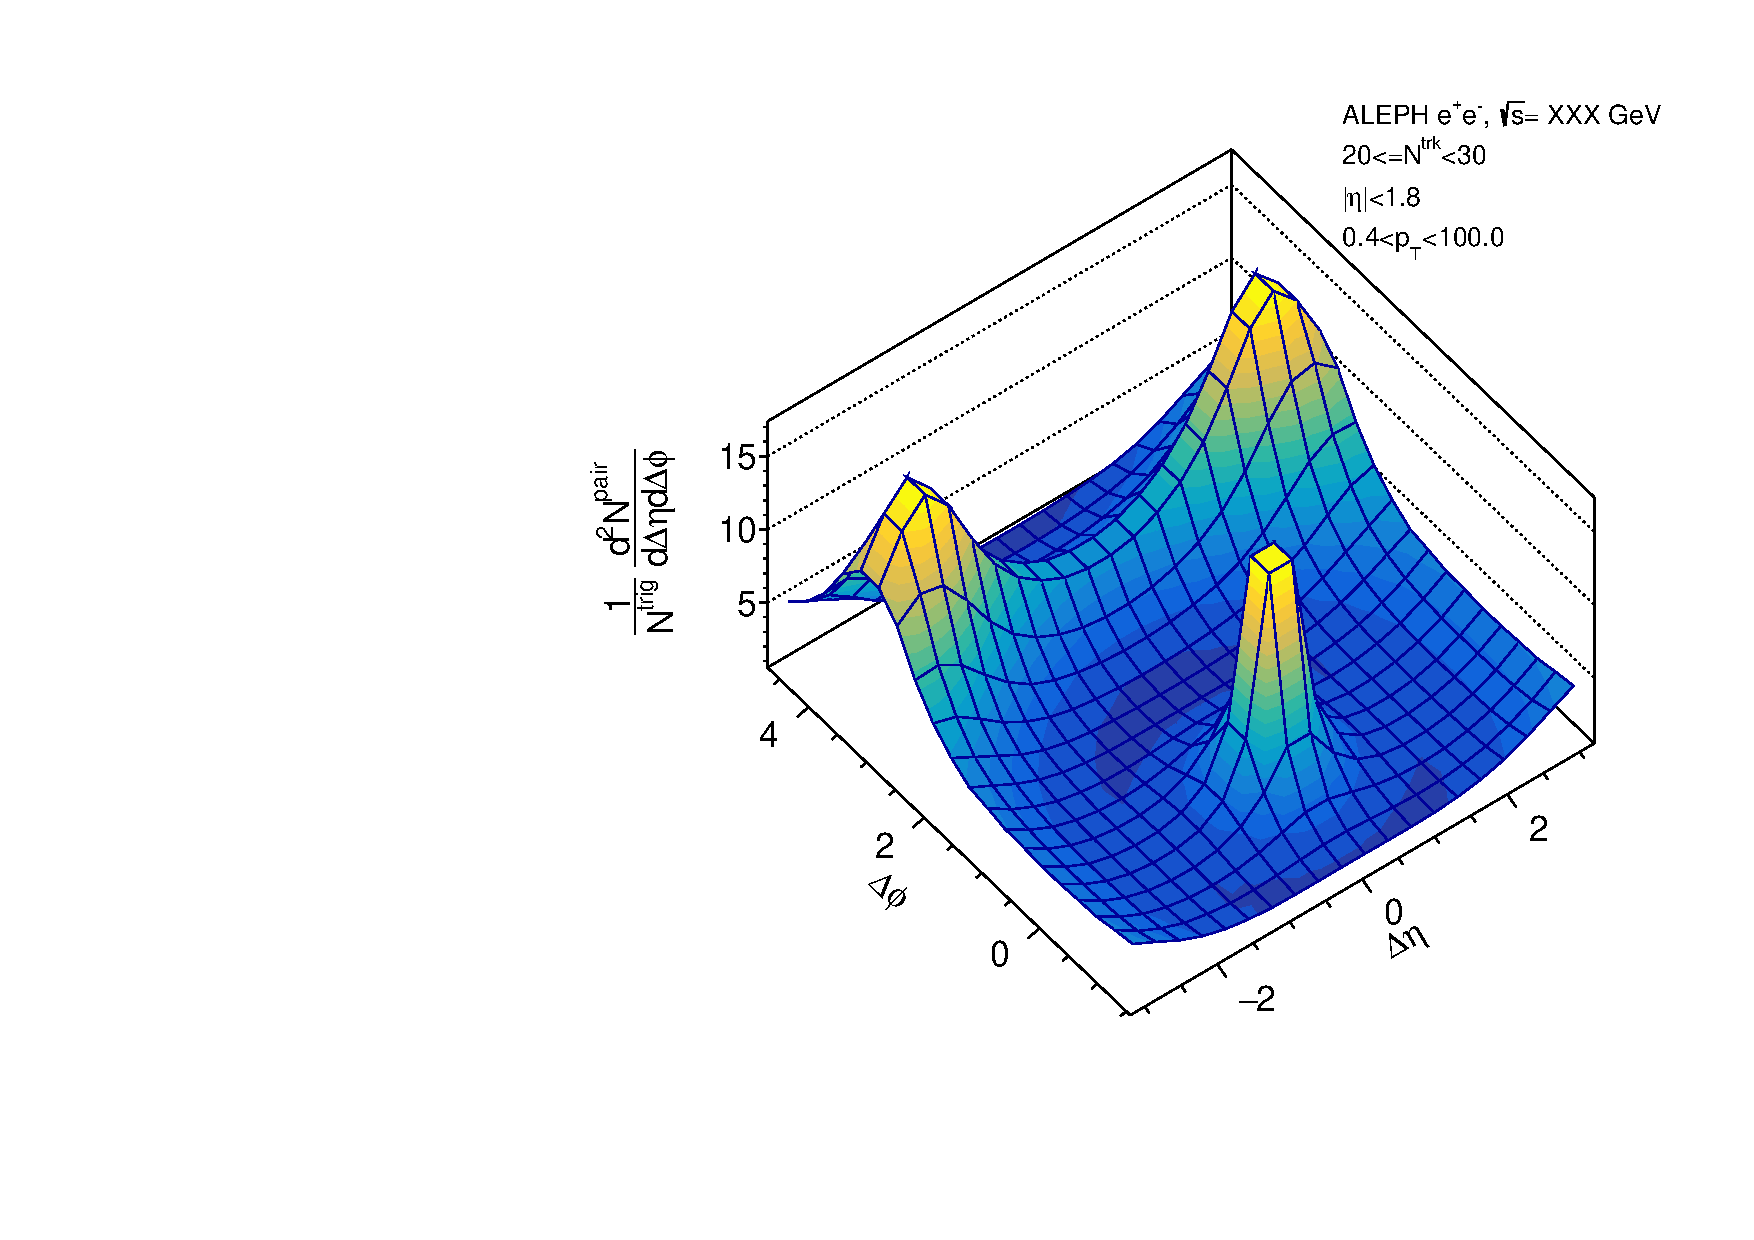
\includegraphics[width=\linewidth]{images/TwoParticleCorrelation/LEP1_BEAM/LEP1_BEAM_ratio2_20_30.pdf}
    \label{fig:LEP1 Beam Axis, Ratio Plot, Multiplicity 20-30, Anthony}
  \end{minipage}
  \begin{minipage}[b]{0.32\linewidth}
    \centering
    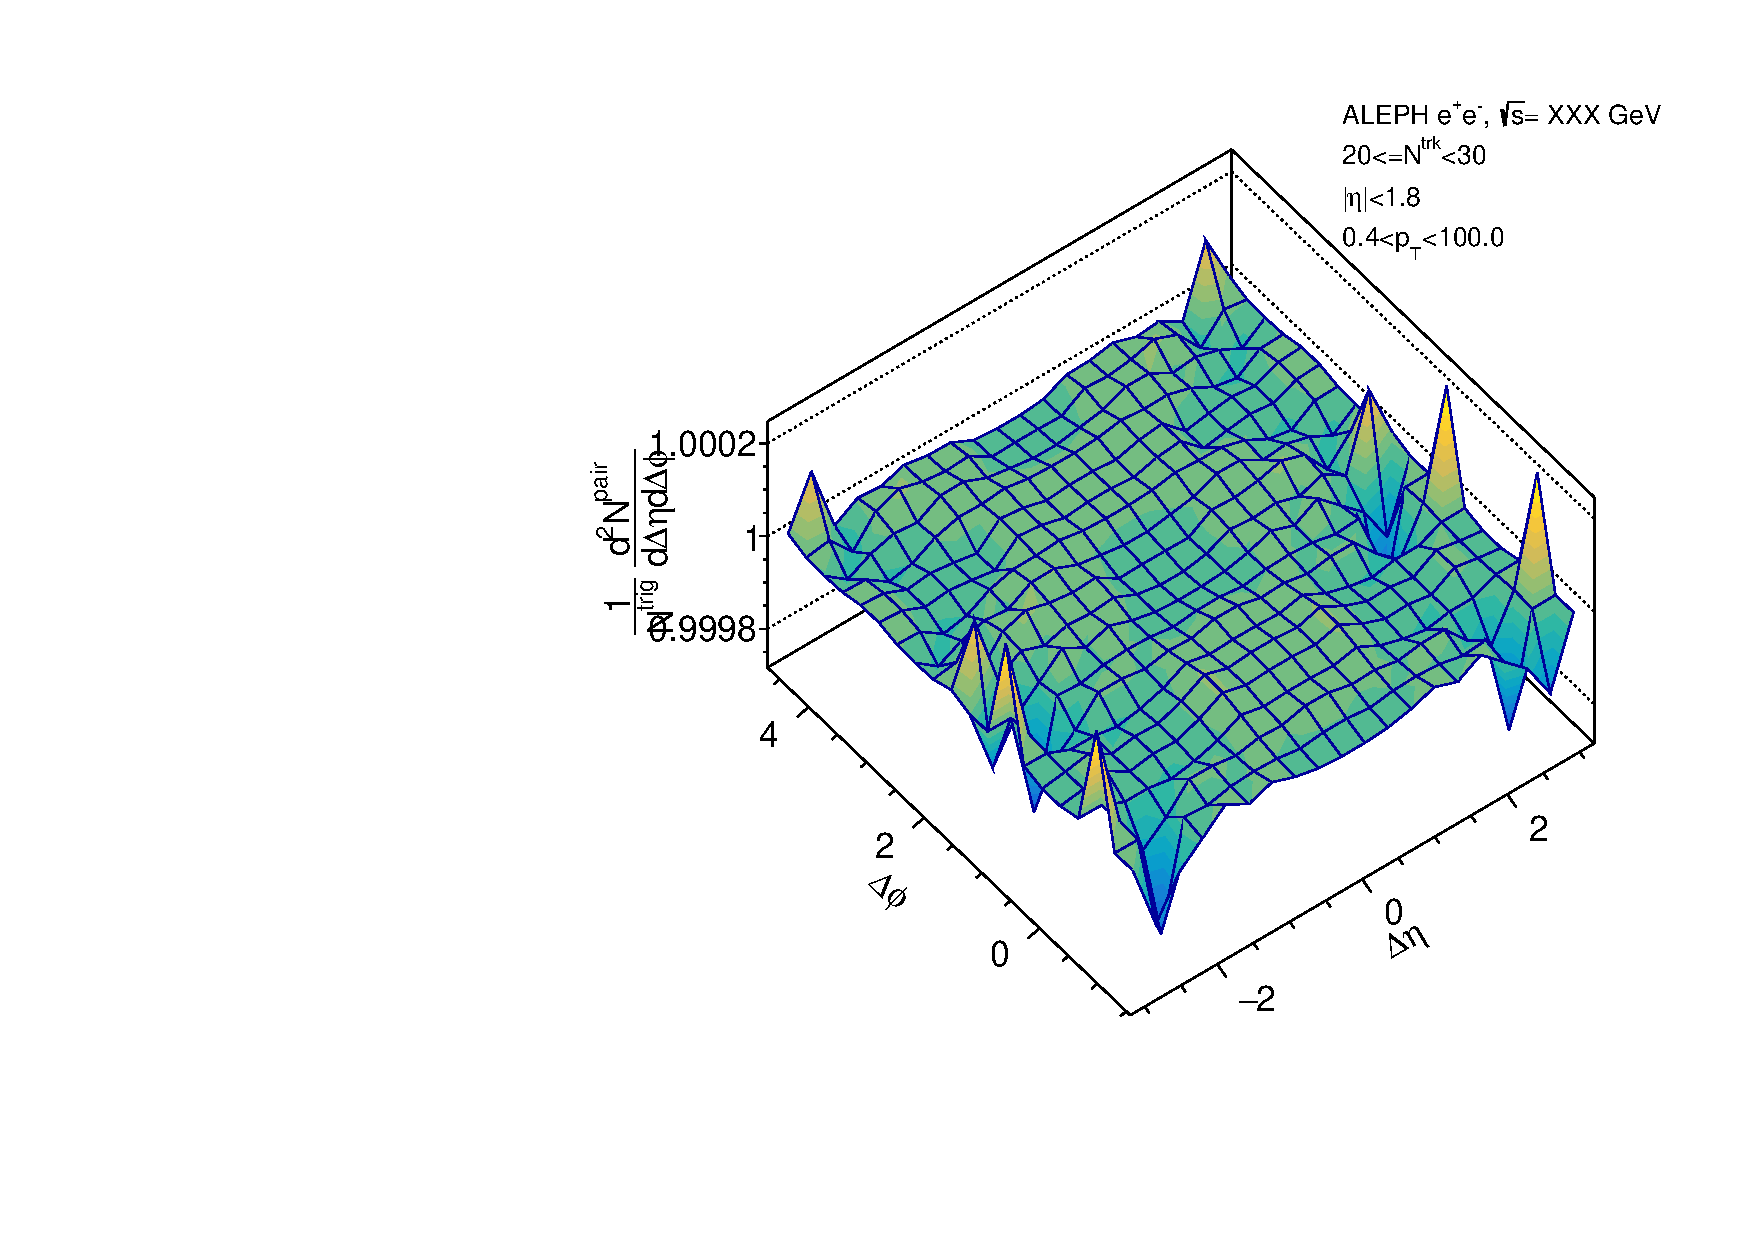
\includegraphics[width=\linewidth]{images/TwoParticleCorrelation/LEP1_BEAM/LEP1_BEAM_r_ratio_20_30.pdf}
    \label{fig:LEP1 Beam Axis, Ratio Plot, Multiplicity 20-30, Ratio}
  \end{minipage}
\end{figure}

%%%%%%%%%%%%%%%%%%%%%%%%%%%%%%%% Multiplicity 30-999 %%%%%%%%%%%%%%%%%%%%%%%%%%%%%%%%
\begin{figure}[htbp]
  \caption{LEP1 Beam Axis, Ratio Plot, Multiplicity 30-999 (Austin, Anthony, Ratio)}
  \begin{minipage}[b]{0.32\linewidth}
    \centering
    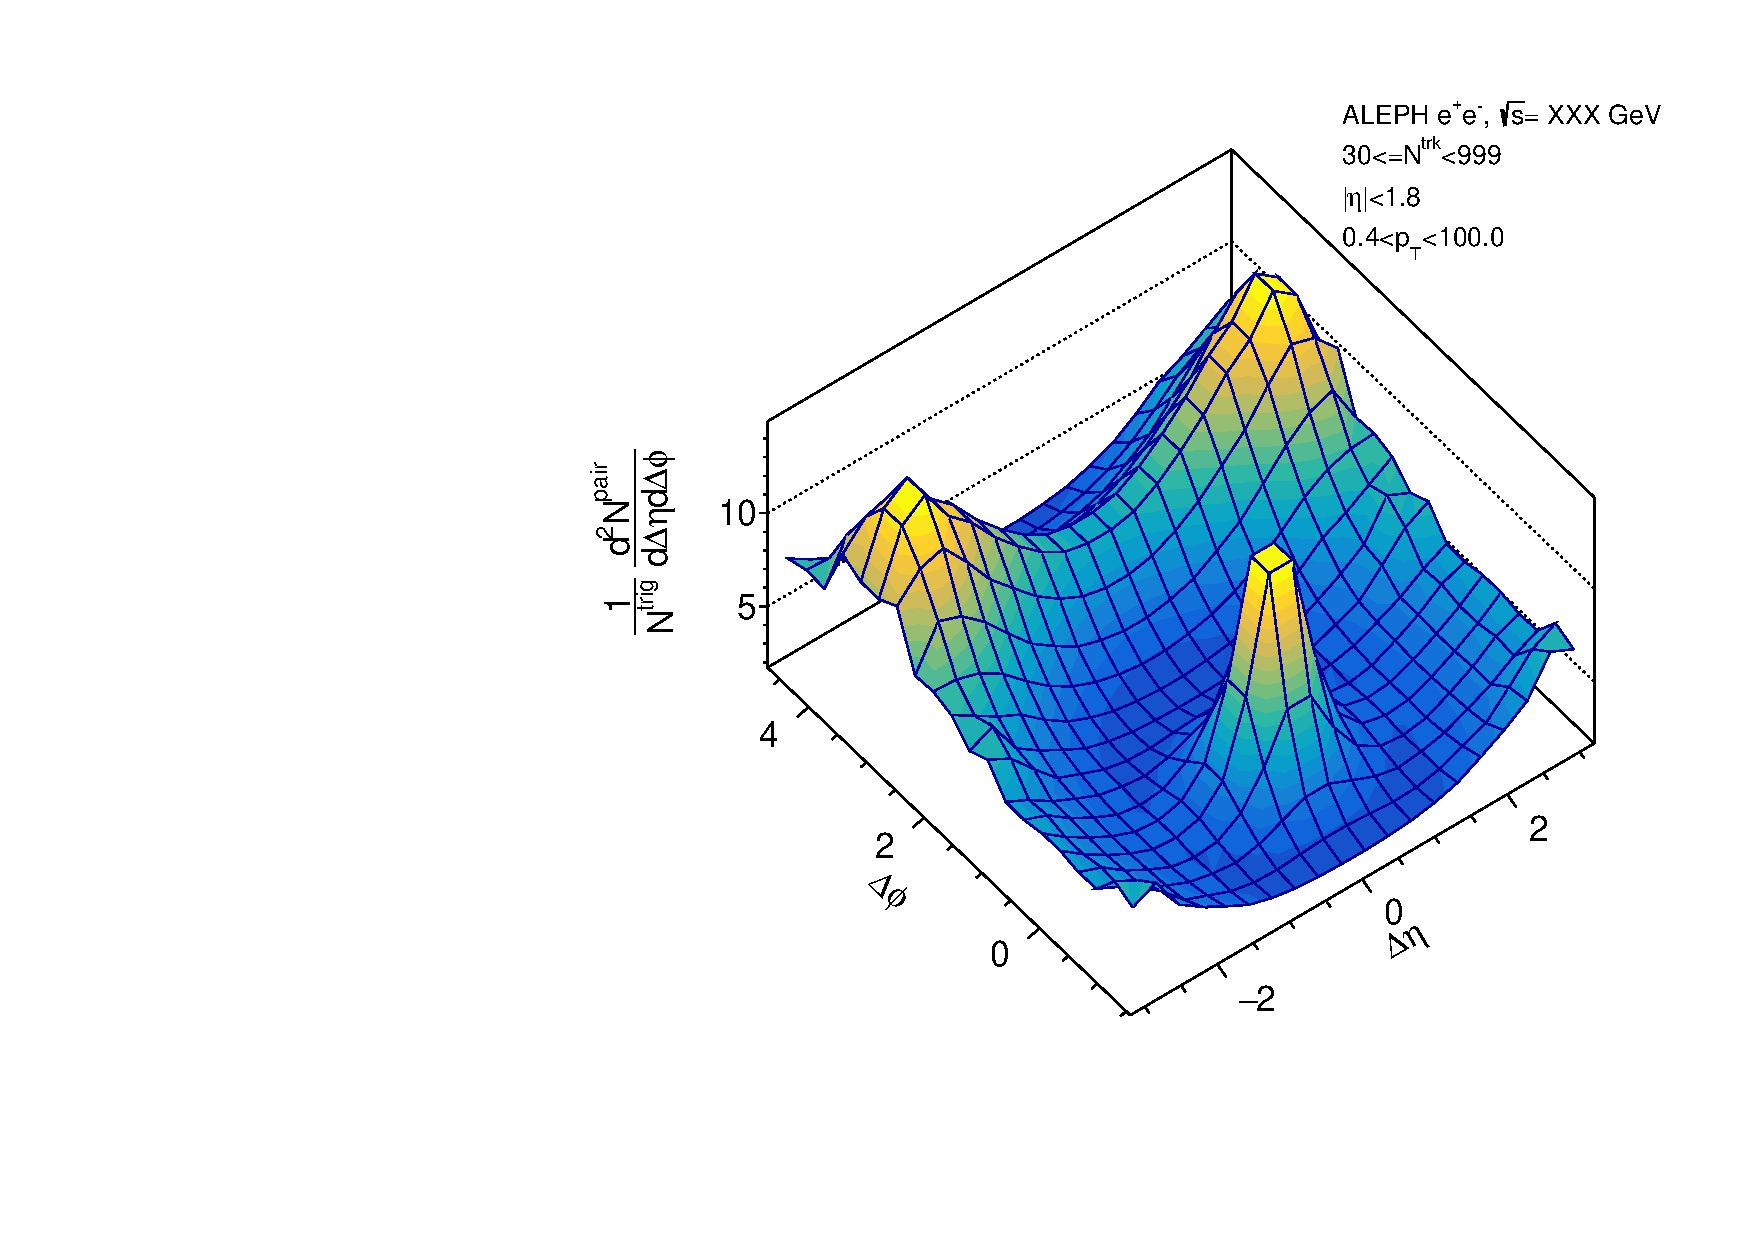
\includegraphics[width=\linewidth]{images/TwoParticleCorrelation/LEP1_BEAM/LEP1_BEAM_ratio1_30_999.pdf}
    \label{fig:LEP1 Beam Axis, Ratio Plot, Multiplicity 30-999, Austin}
  \end{minipage}
  \hspace{0.0cm}
  \begin{minipage}[b]{0.32\linewidth}
    \centering
    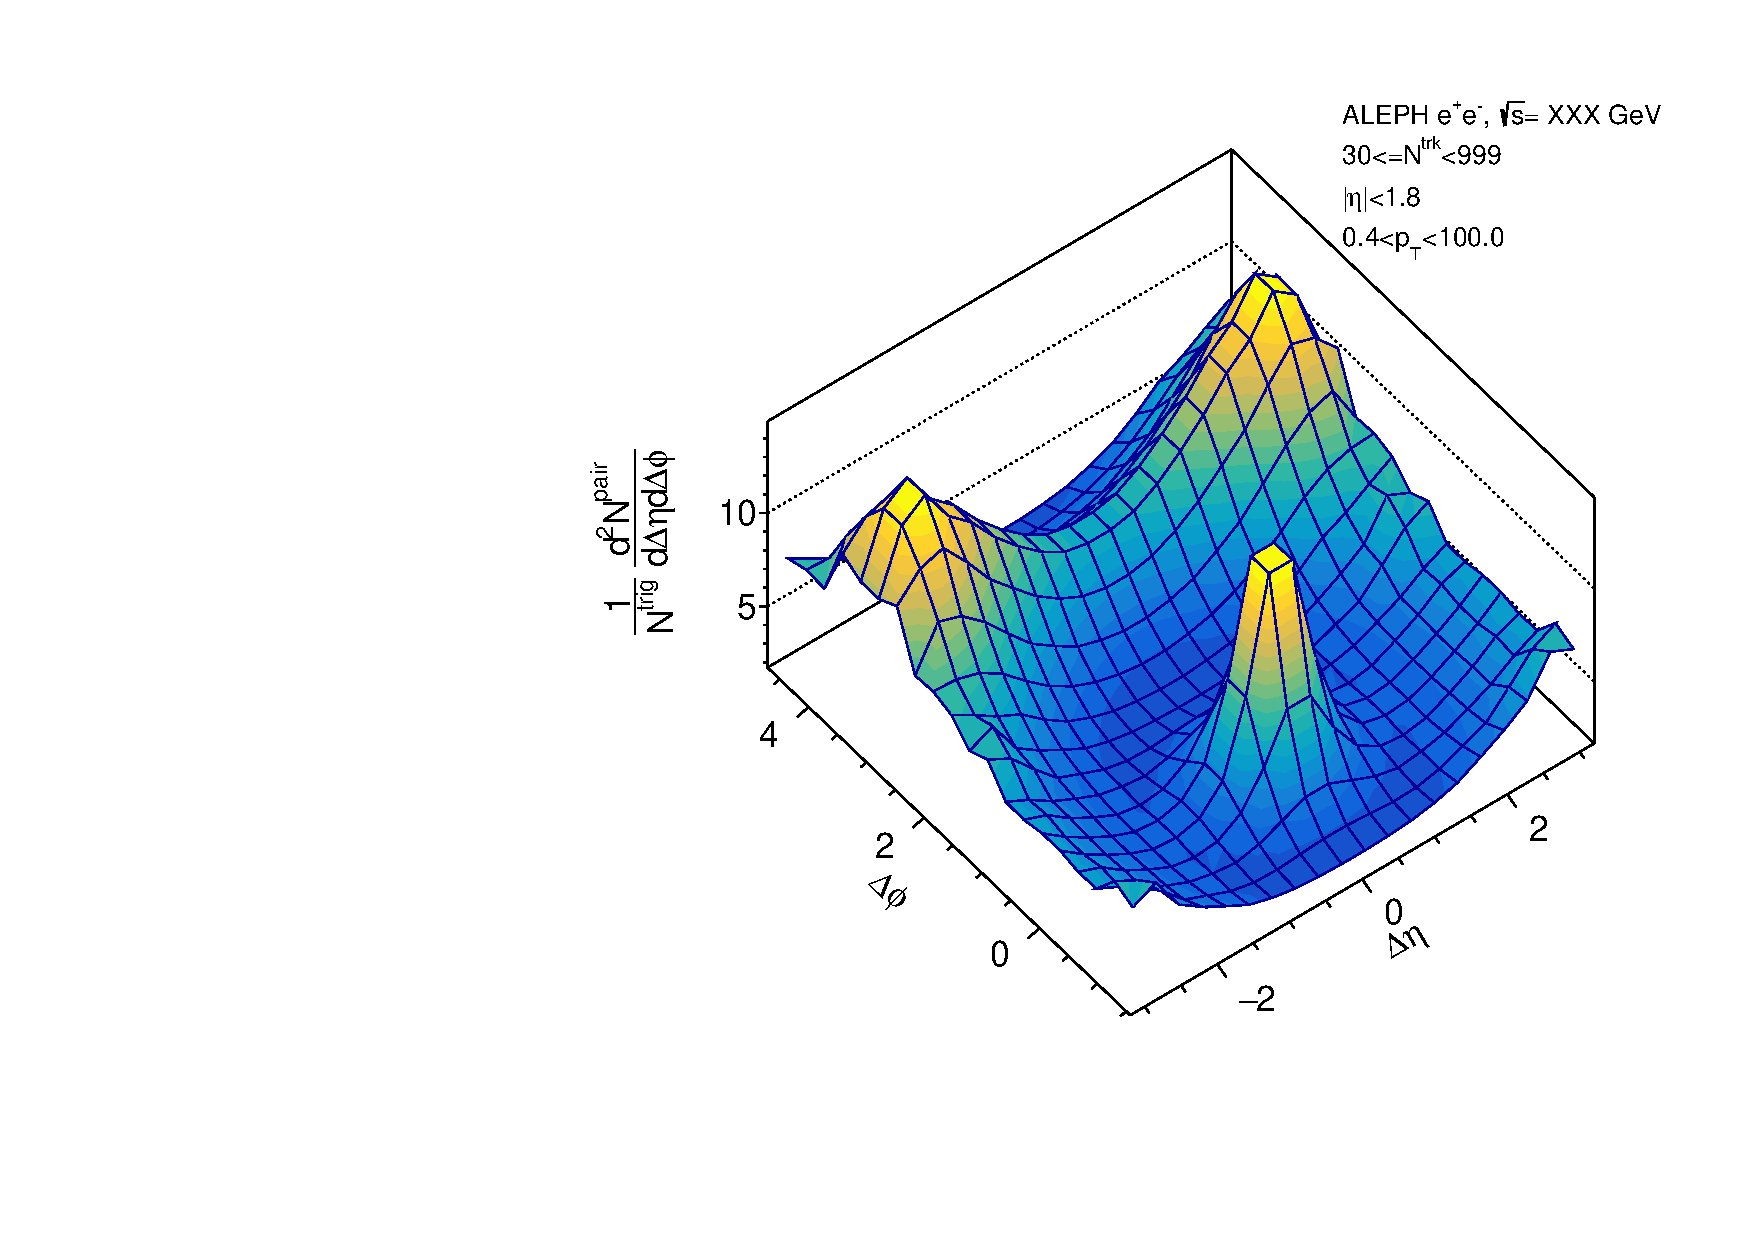
\includegraphics[width=\linewidth]{images/TwoParticleCorrelation/LEP1_BEAM/LEP1_BEAM_ratio2_30_999.pdf}
    \label{fig:LEP1 Beam Axis, Ratio Plot, Multiplicity 30-999, Anthony}
  \end{minipage}
  \begin{minipage}[b]{0.32\linewidth}
    \centering
    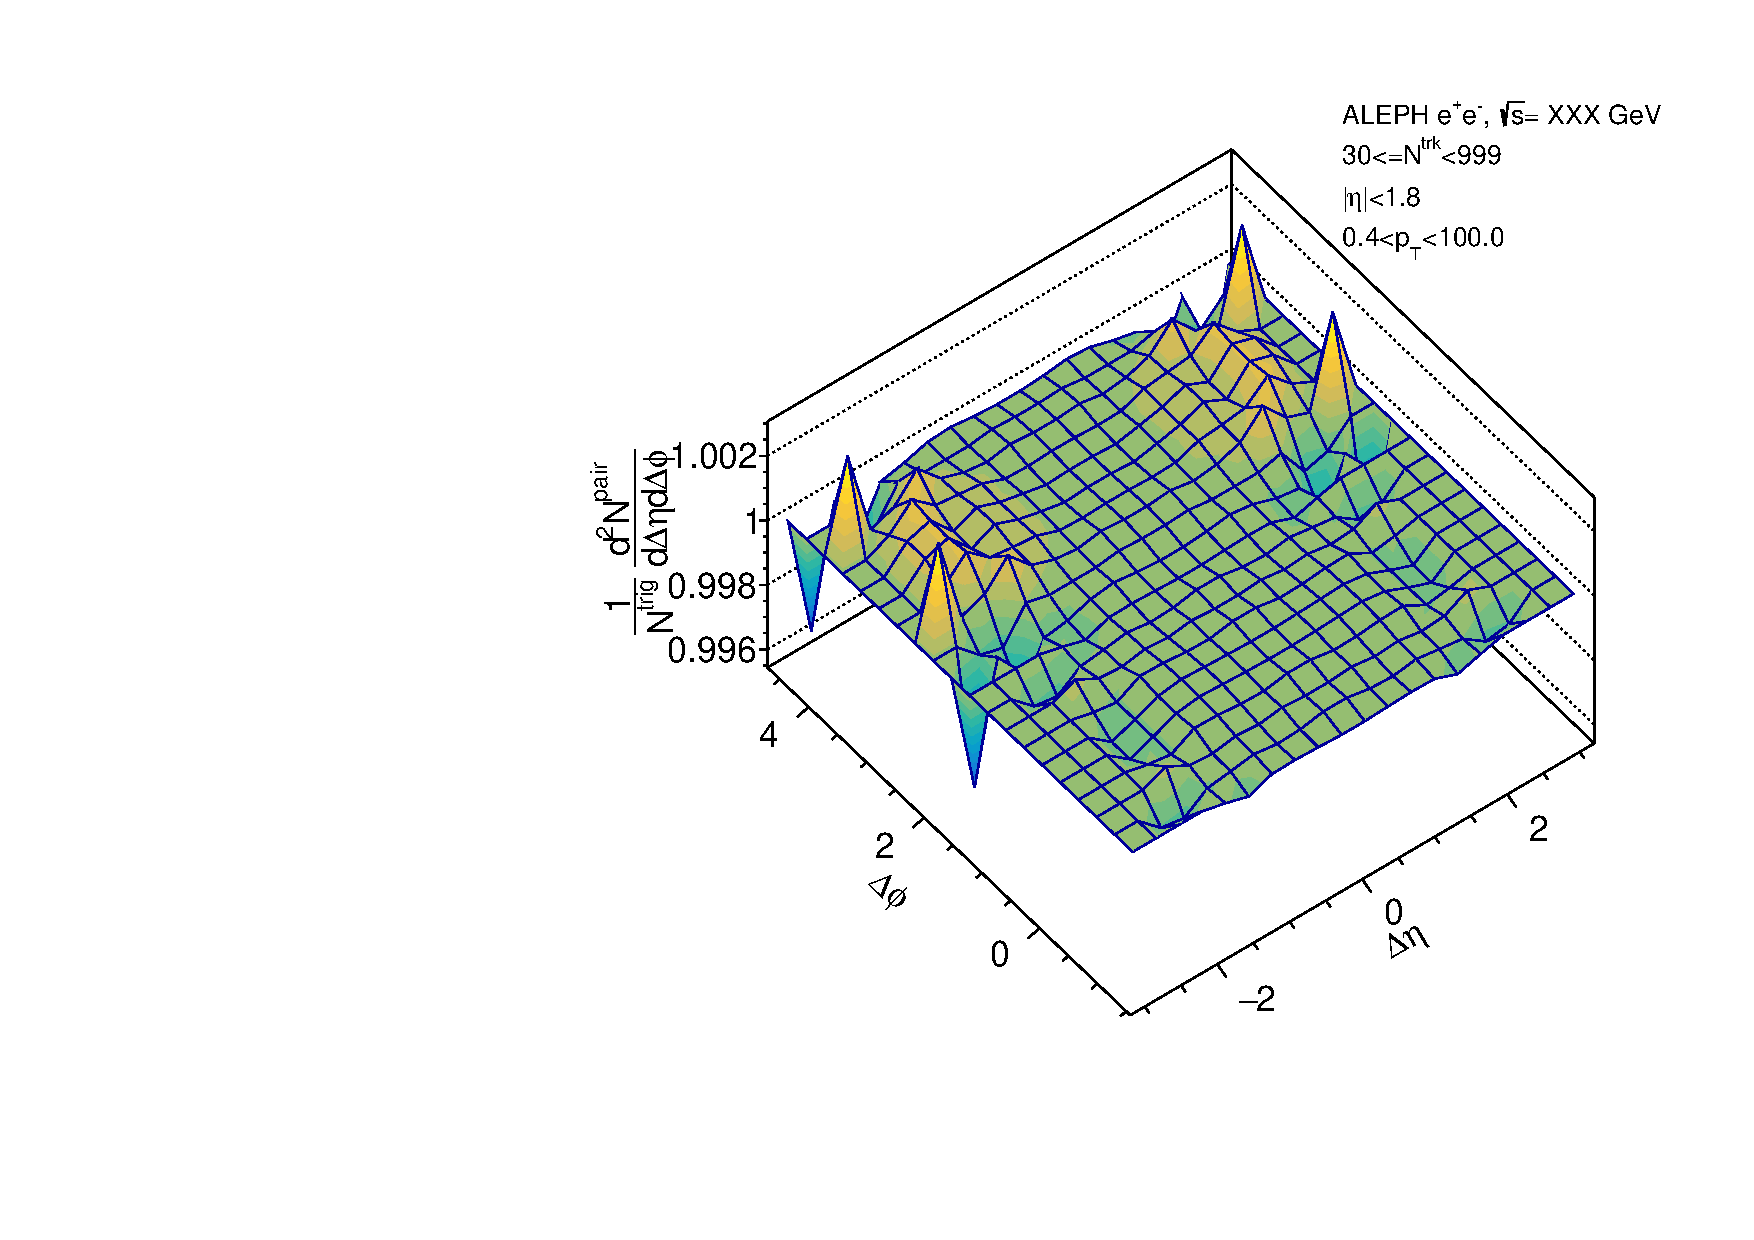
\includegraphics[width=\linewidth]{images/TwoParticleCorrelation/LEP1_BEAM/LEP1_BEAM_r_ratio_30_999.pdf}
    \label{fig:LEP1 Beam Axis, Ratio Plot, Multiplicity 30-999, Ratio}
  \end{minipage}
\end{figure}


%%%%%%%%%%%%%%%%%%%%%%%%%%%%%%%%%%%%%%%%%%%%%%%%%%%%%%%%%%%%%%%% LEP1 THRUST AXIS %%%%%%%%%%%%%%%%%%%%%%%%%%%%%%%%%%%%%%%%%%%%%%%%%%%%%%%%%%%%%%%%
%%%%%%%%%%%%%%%%%%%%%%%%%%%%%%%% Multiplicity 0-20 %%%%%%%%%%%%%%%%%%%%%%%%%%%%%%%%
\begin{figure}[htbp]
  \caption{LEP1 Thrust Axis, Ratio Plot, Multiplicity 0-20 (Austin, Anthony, Ratio)}
  \begin{minipage}[b]{0.32\linewidth}
    \centering
    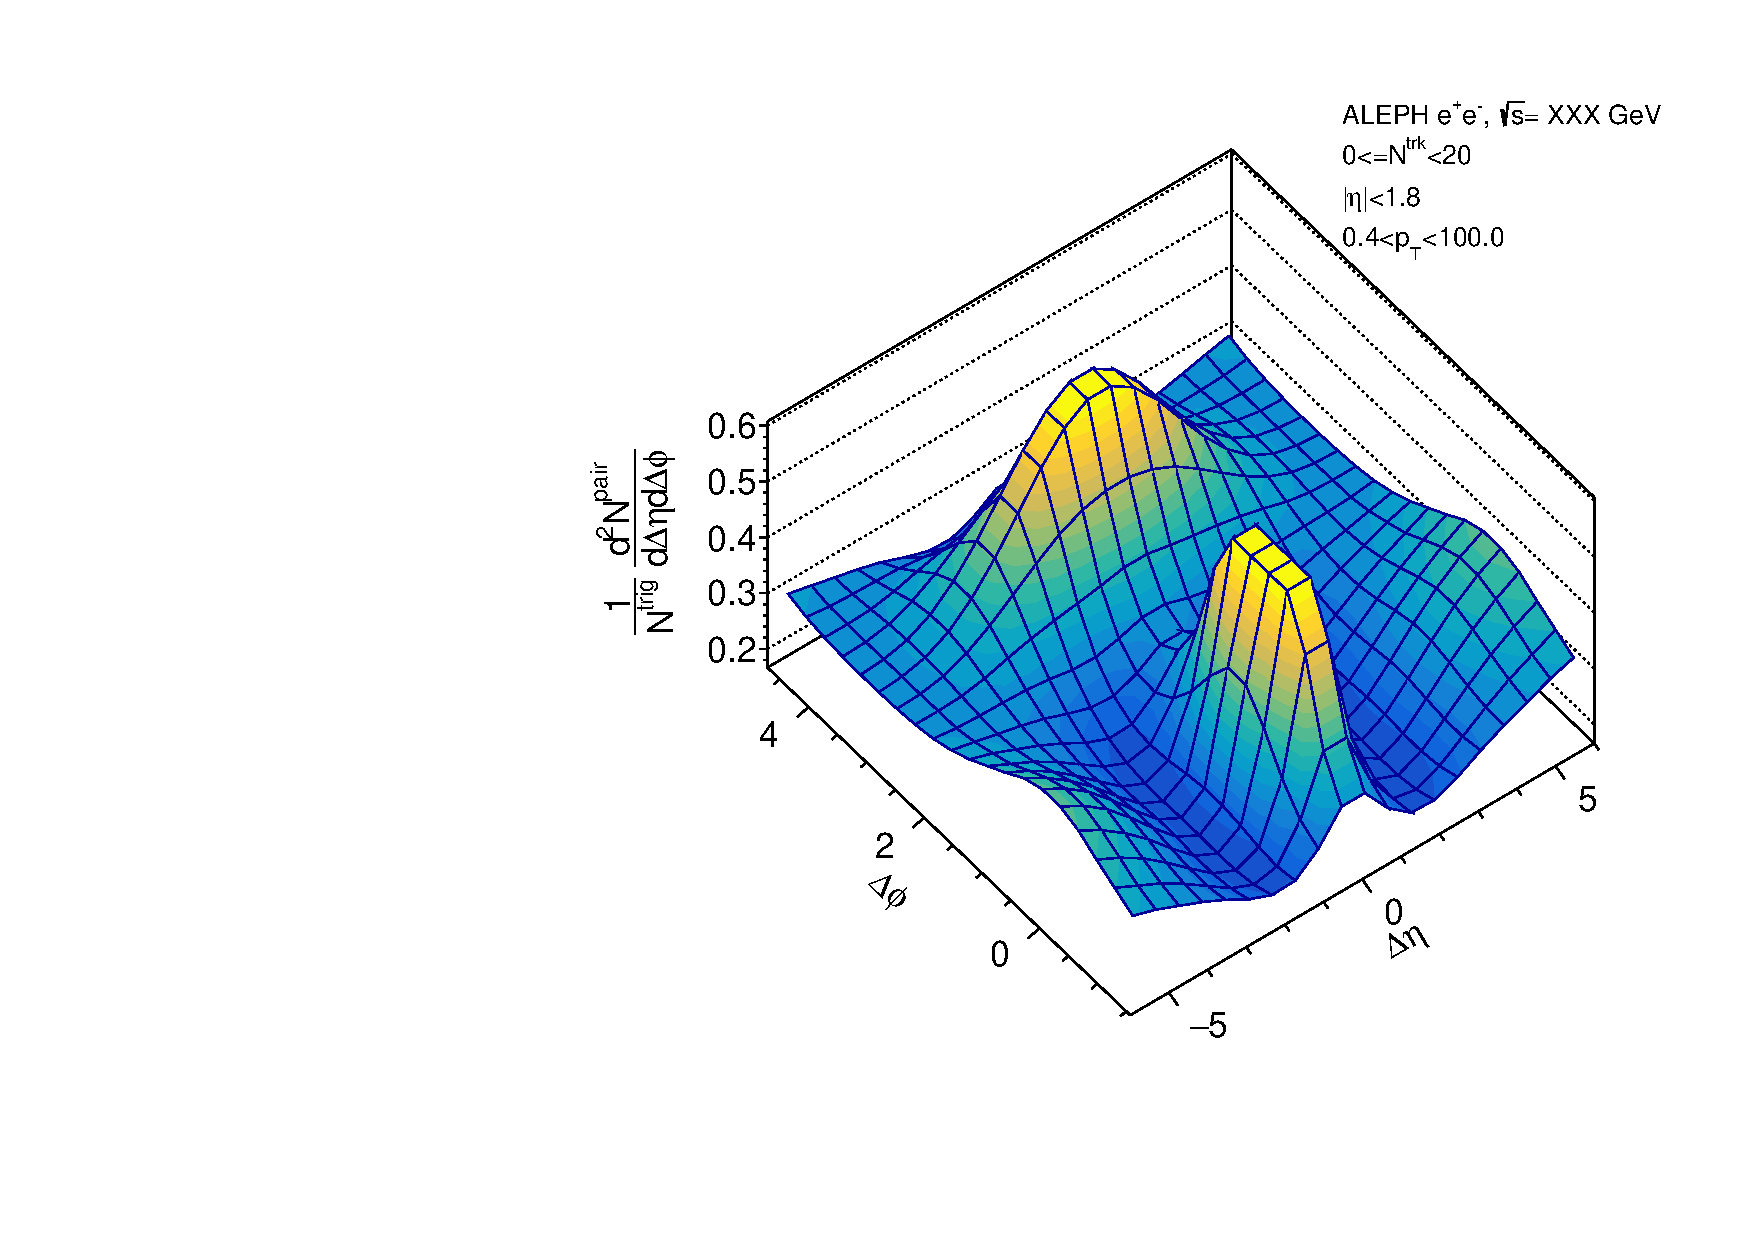
\includegraphics[width=\linewidth]{images/TwoParticleCorrelation/LEP1_THRUST/LEP1_THRUST_ratio1_0_20.pdf}  
    \label{fig:LEP1 Thrust Axis, Ratio Plot, Multiplicity 0-20, Austin}
  \end{minipage}
  \hspace{0.0cm}
  \begin{minipage}[b]{0.32\linewidth}
    \centering
    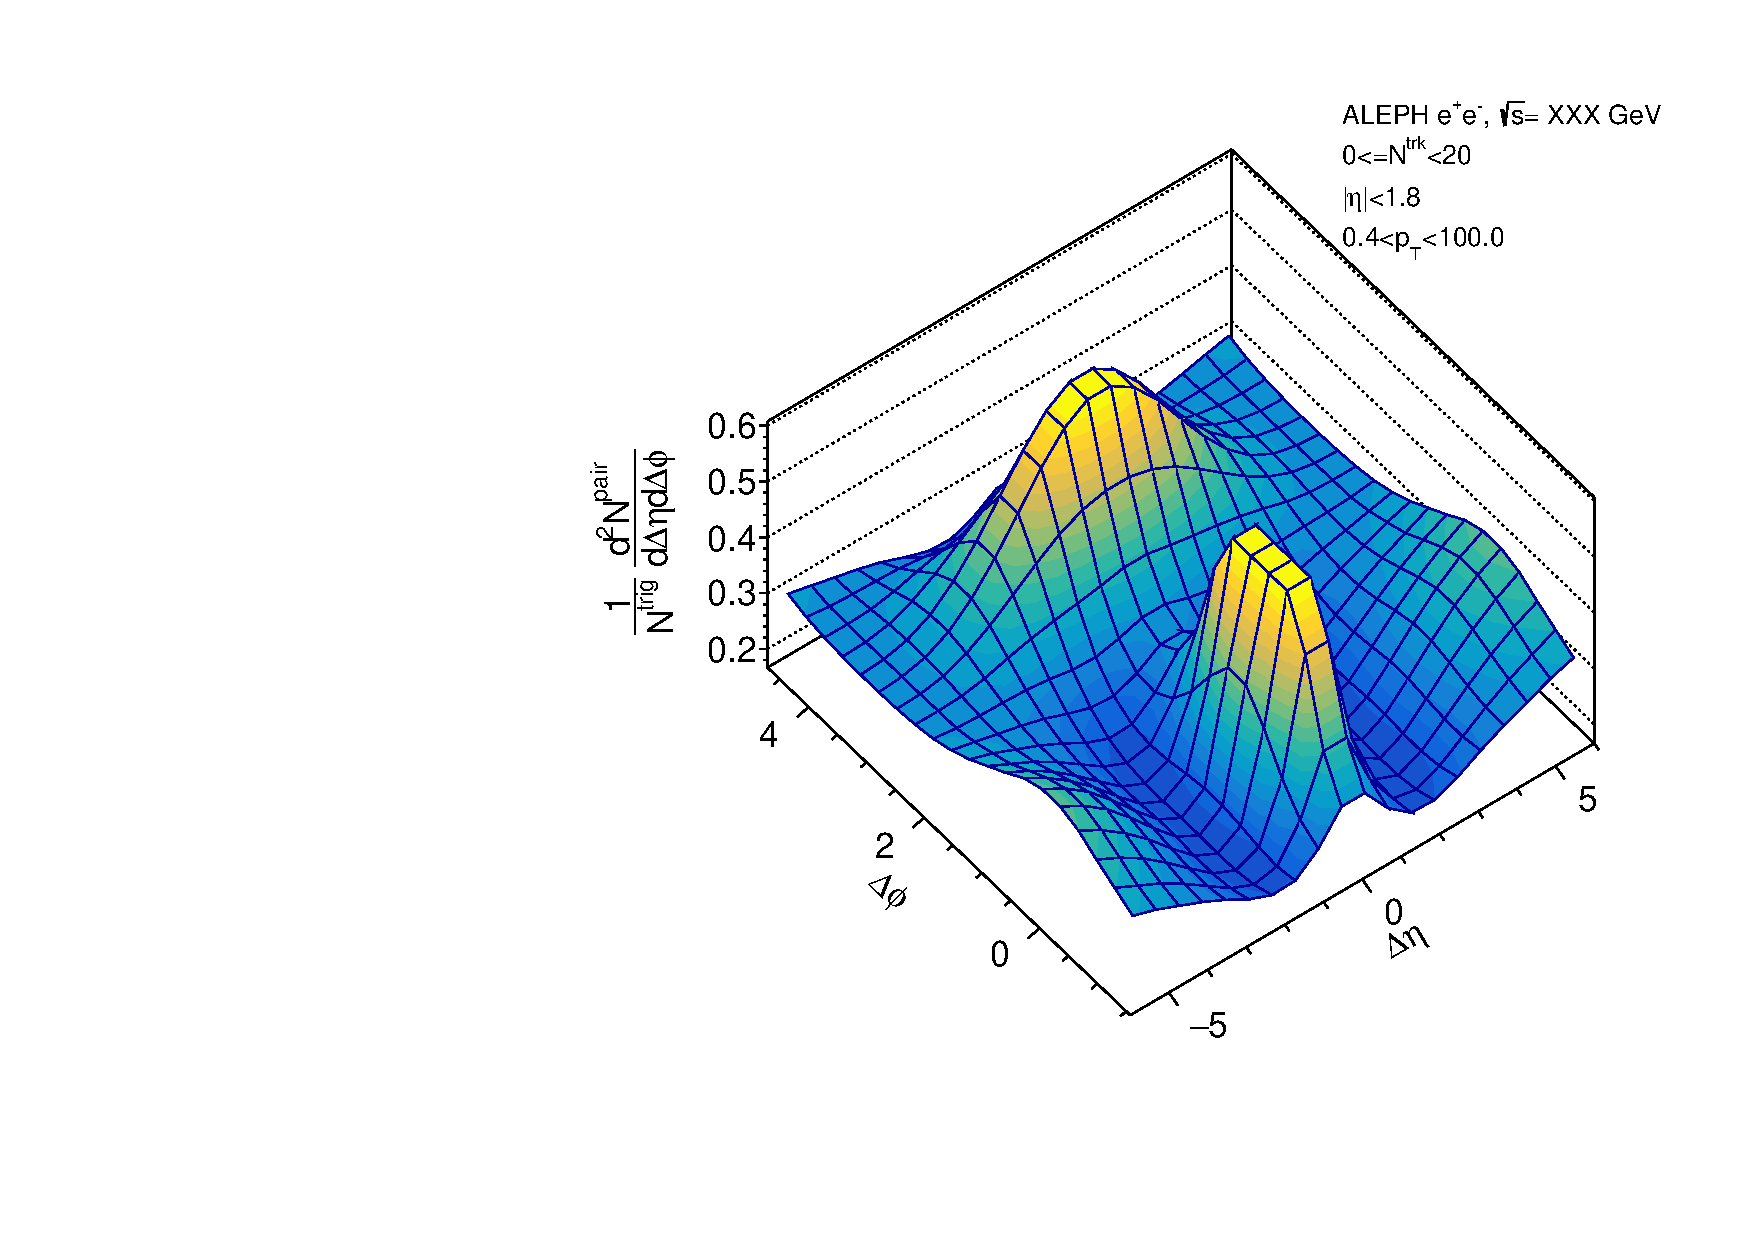
\includegraphics[width=\linewidth]{images/TwoParticleCorrelation/LEP1_THRUST/LEP1_THRUST_ratio2_0_20.pdf}
    \label{fig:LEP1 Thrust Axis, Ratio Plot, Multiplicity 0-20, Anthony}
  \end{minipage}
  \begin{minipage}[b]{0.32\linewidth}
    \centering
    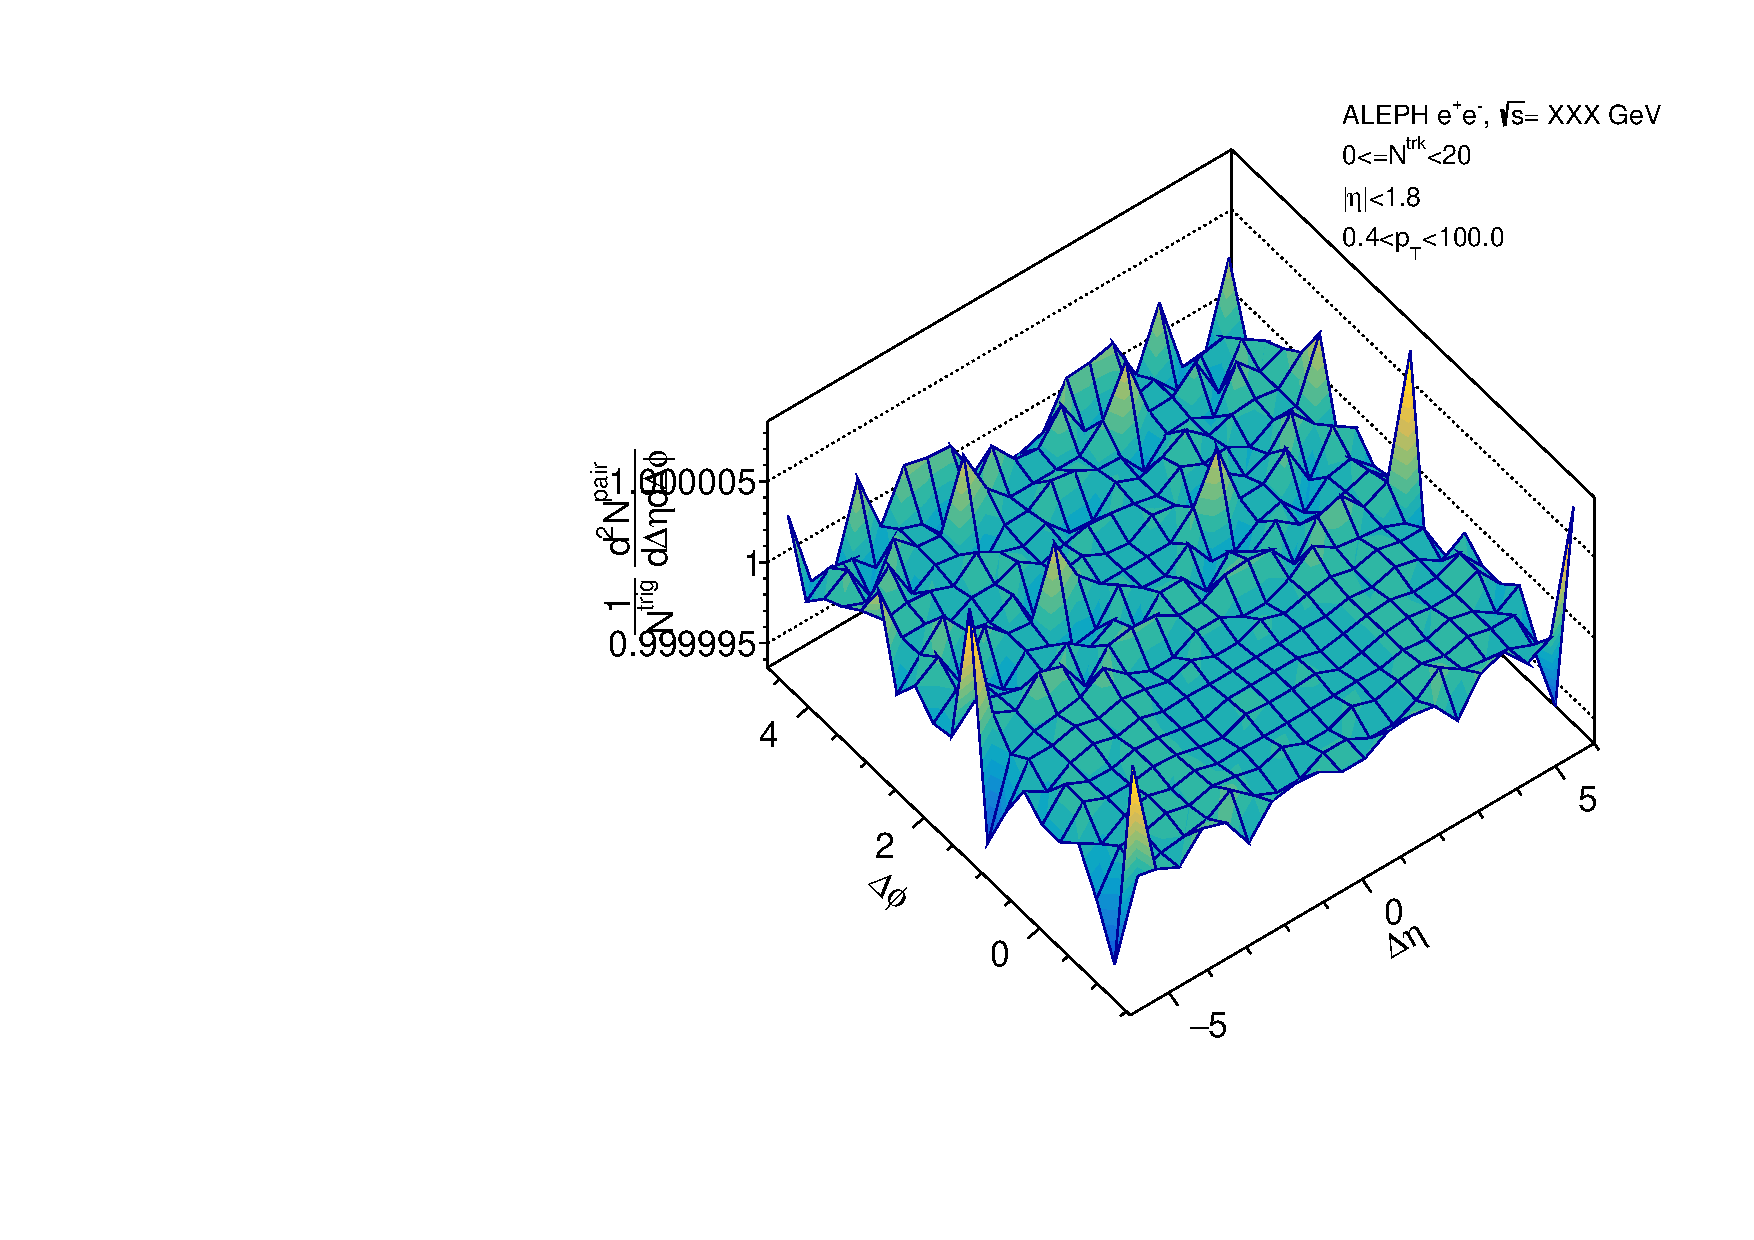
\includegraphics[width=\linewidth]{images/TwoParticleCorrelation/LEP1_THRUST/LEP1_THRUST_r_ratio_0_20.pdf}
    \label{fig:LEP1 Thrust Axis, Ratio Plot, Multiplicity 0-20, Ratio}
  \end{minipage}
\end{figure}


%%%%%%%%%%%%%%%%%%%%%%%%%%%%%%%% Multiplicity 20-30 %%%%%%%%%%%%%%%%%%%%%%%%%%%%%%%%
\begin{figure}[htbp]
  \caption{LEP1 Thrust Axis, Ratio Plot, Multiplicity 20-30 (Austin, Anthony, Ratio)}
  \begin{minipage}[b]{0.32\linewidth}
    \centering
    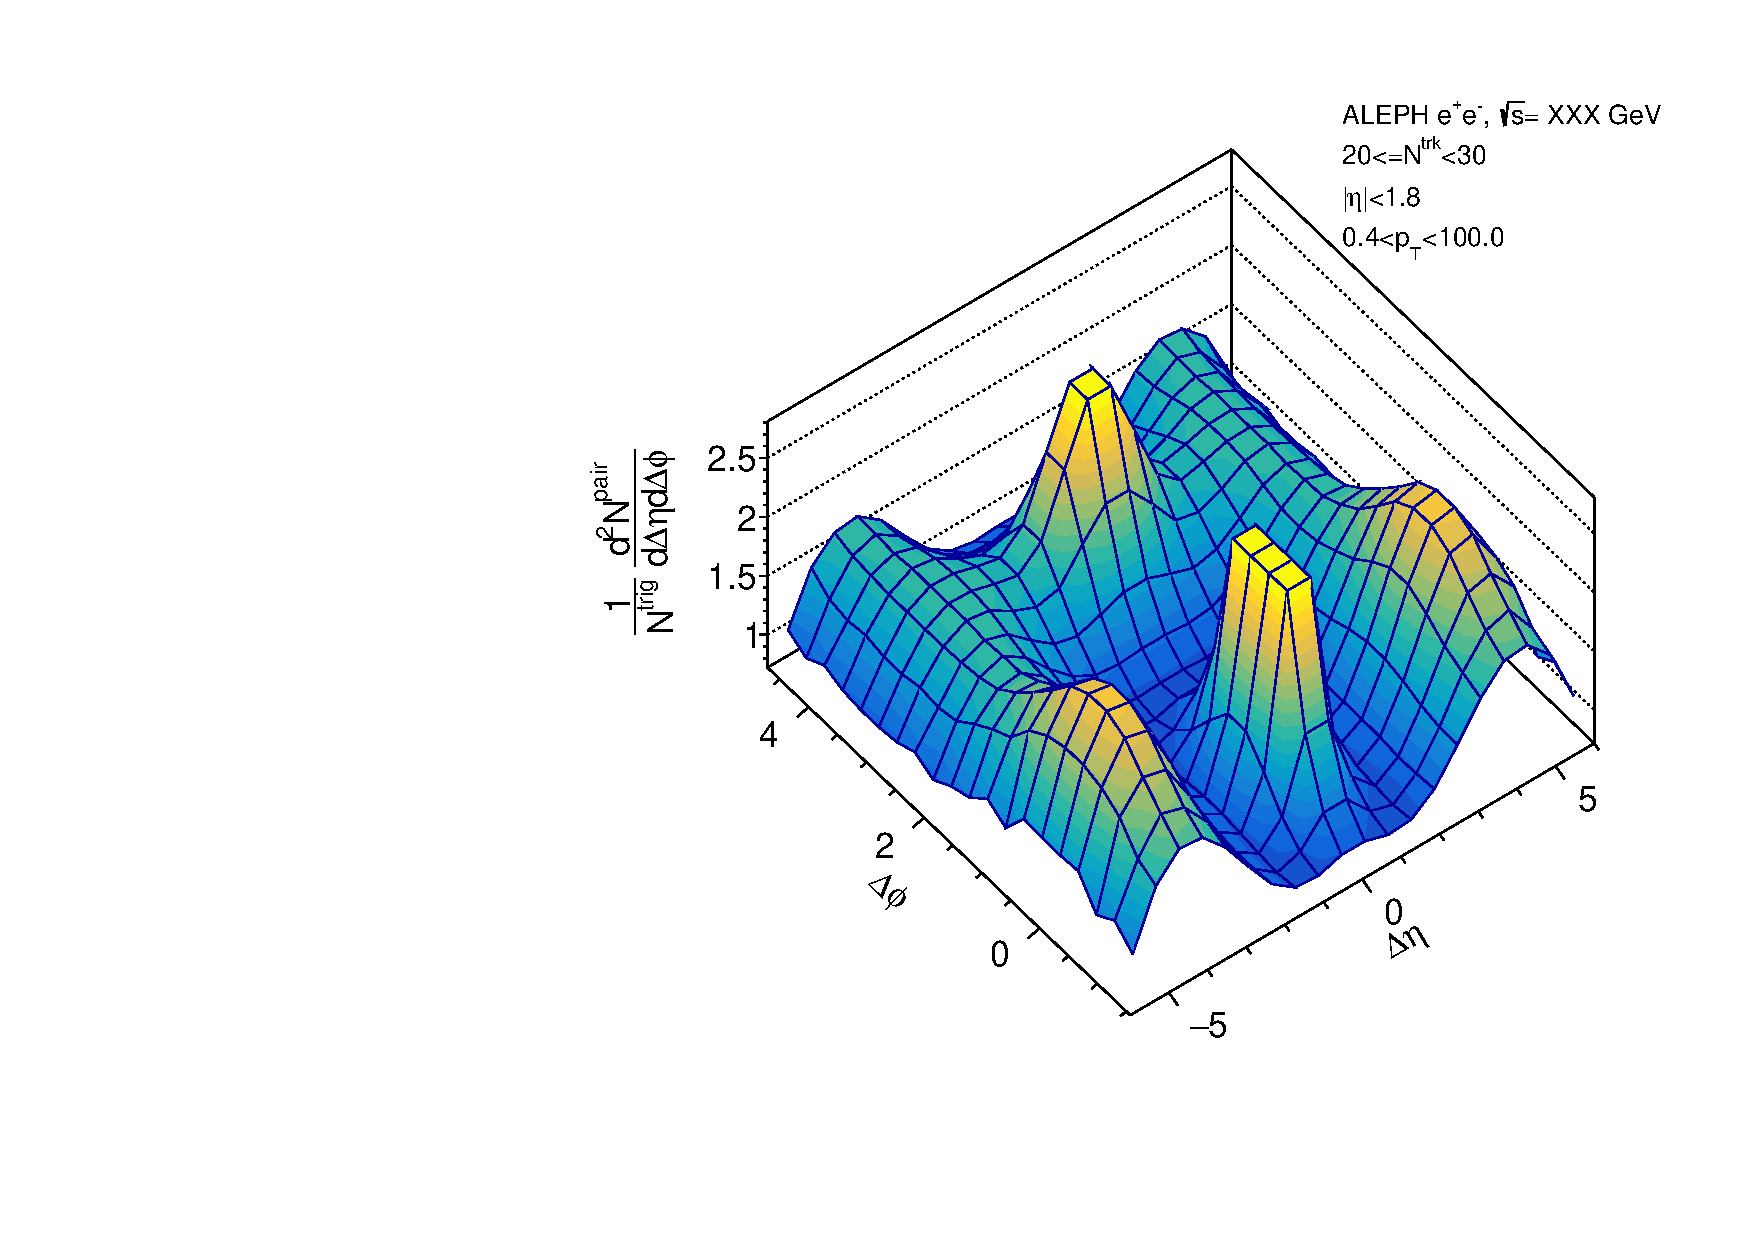
\includegraphics[width=\linewidth]{images/TwoParticleCorrelation/LEP1_THRUST/LEP1_THRUST_ratio1_20_30.pdf}
    \label{fig:LEP1 Thrust Axis, Ratio Plot, Multiplicity 20-30, Austin}
  \end{minipage}
  \hspace{0.0cm}
  \begin{minipage}[b]{0.32\linewidth}
    \centering
    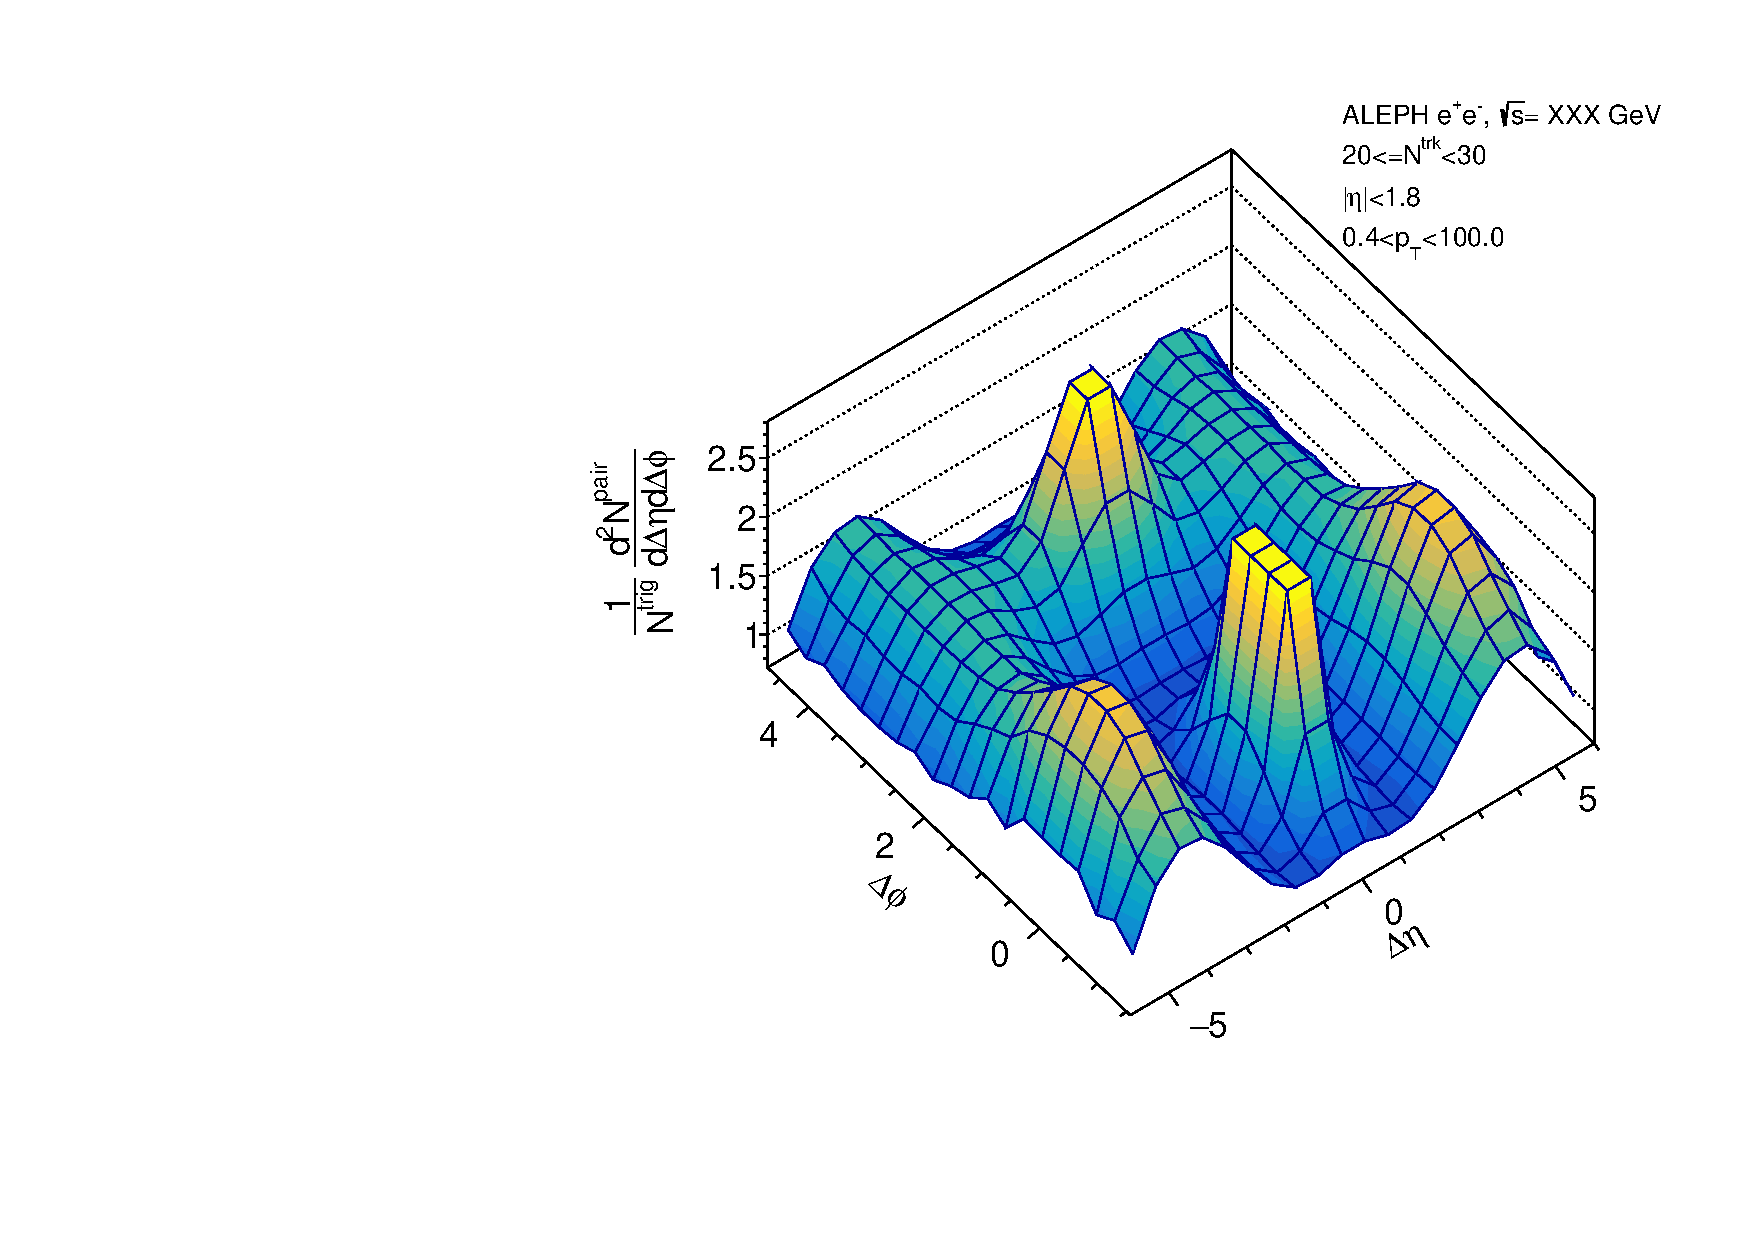
\includegraphics[width=\linewidth]{images/TwoParticleCorrelation/LEP1_THRUST/LEP1_THRUST_ratio2_20_30.pdf}
    \label{fig:LEP1 Thrust Axis, Ratio Plot, Multiplicity 20-30, Anthony}
  \end{minipage}
  \begin{minipage}[b]{0.32\linewidth}
    \centering
    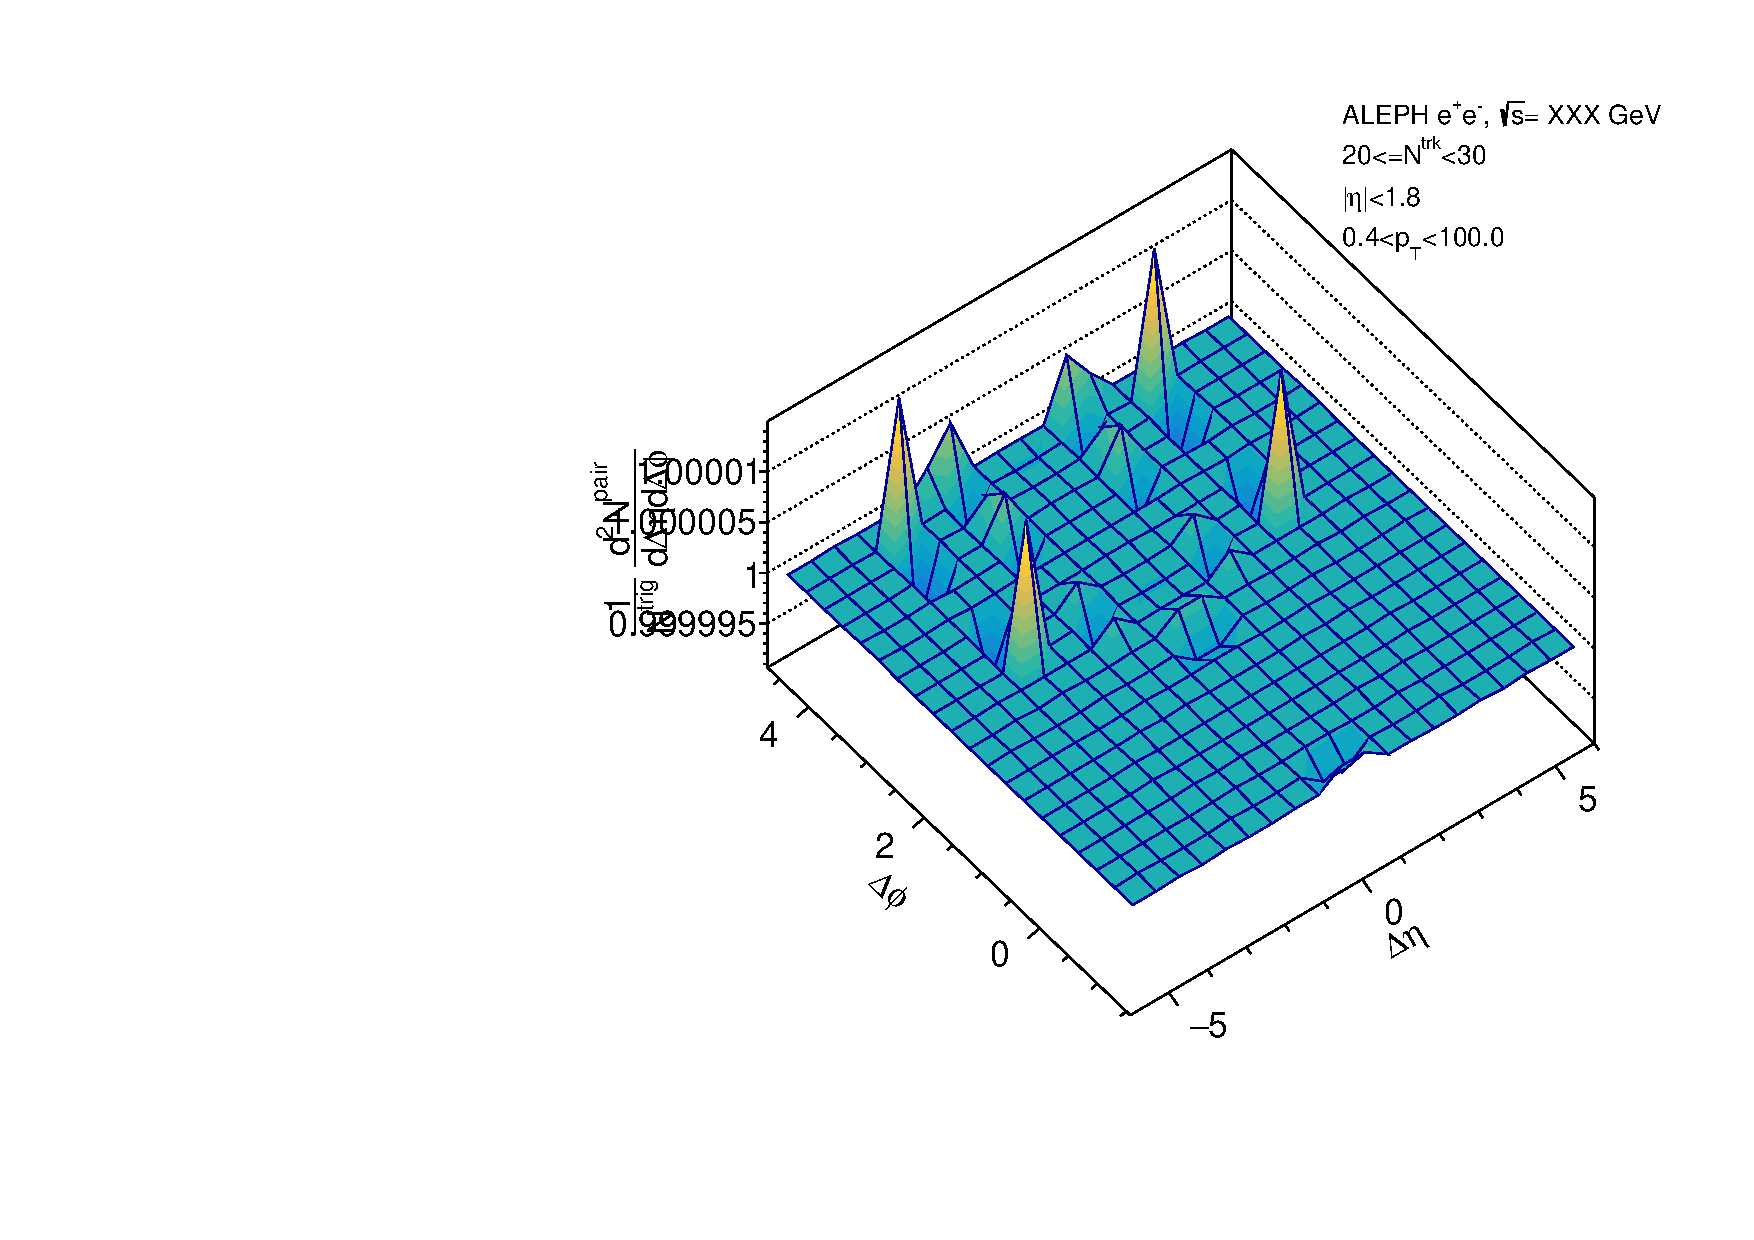
\includegraphics[width=\linewidth]{images/TwoParticleCorrelation/LEP1_THRUST/LEP1_THRUST_r_ratio_20_30.pdf}
    \label{fig:LEP1 Thrust Axis, Ratio Plot, Multiplicity 20-30, Ratio}
  \end{minipage}
\end{figure}

%%%%%%%%%%%%%%%%%%%%%%%%%%%%%%%% Multiplicity 30-999 %%%%%%%%%%%%%%%%%%%%%%%%%%%%%%%%
\begin{figure}[htbp]
  \caption{LEP1 Thrust Axis, Ratio Plot, Multiplicity 30-999 (Austin, Anthony, Ratio)}
  \begin{minipage}[b]{0.32\linewidth}
    \centering
    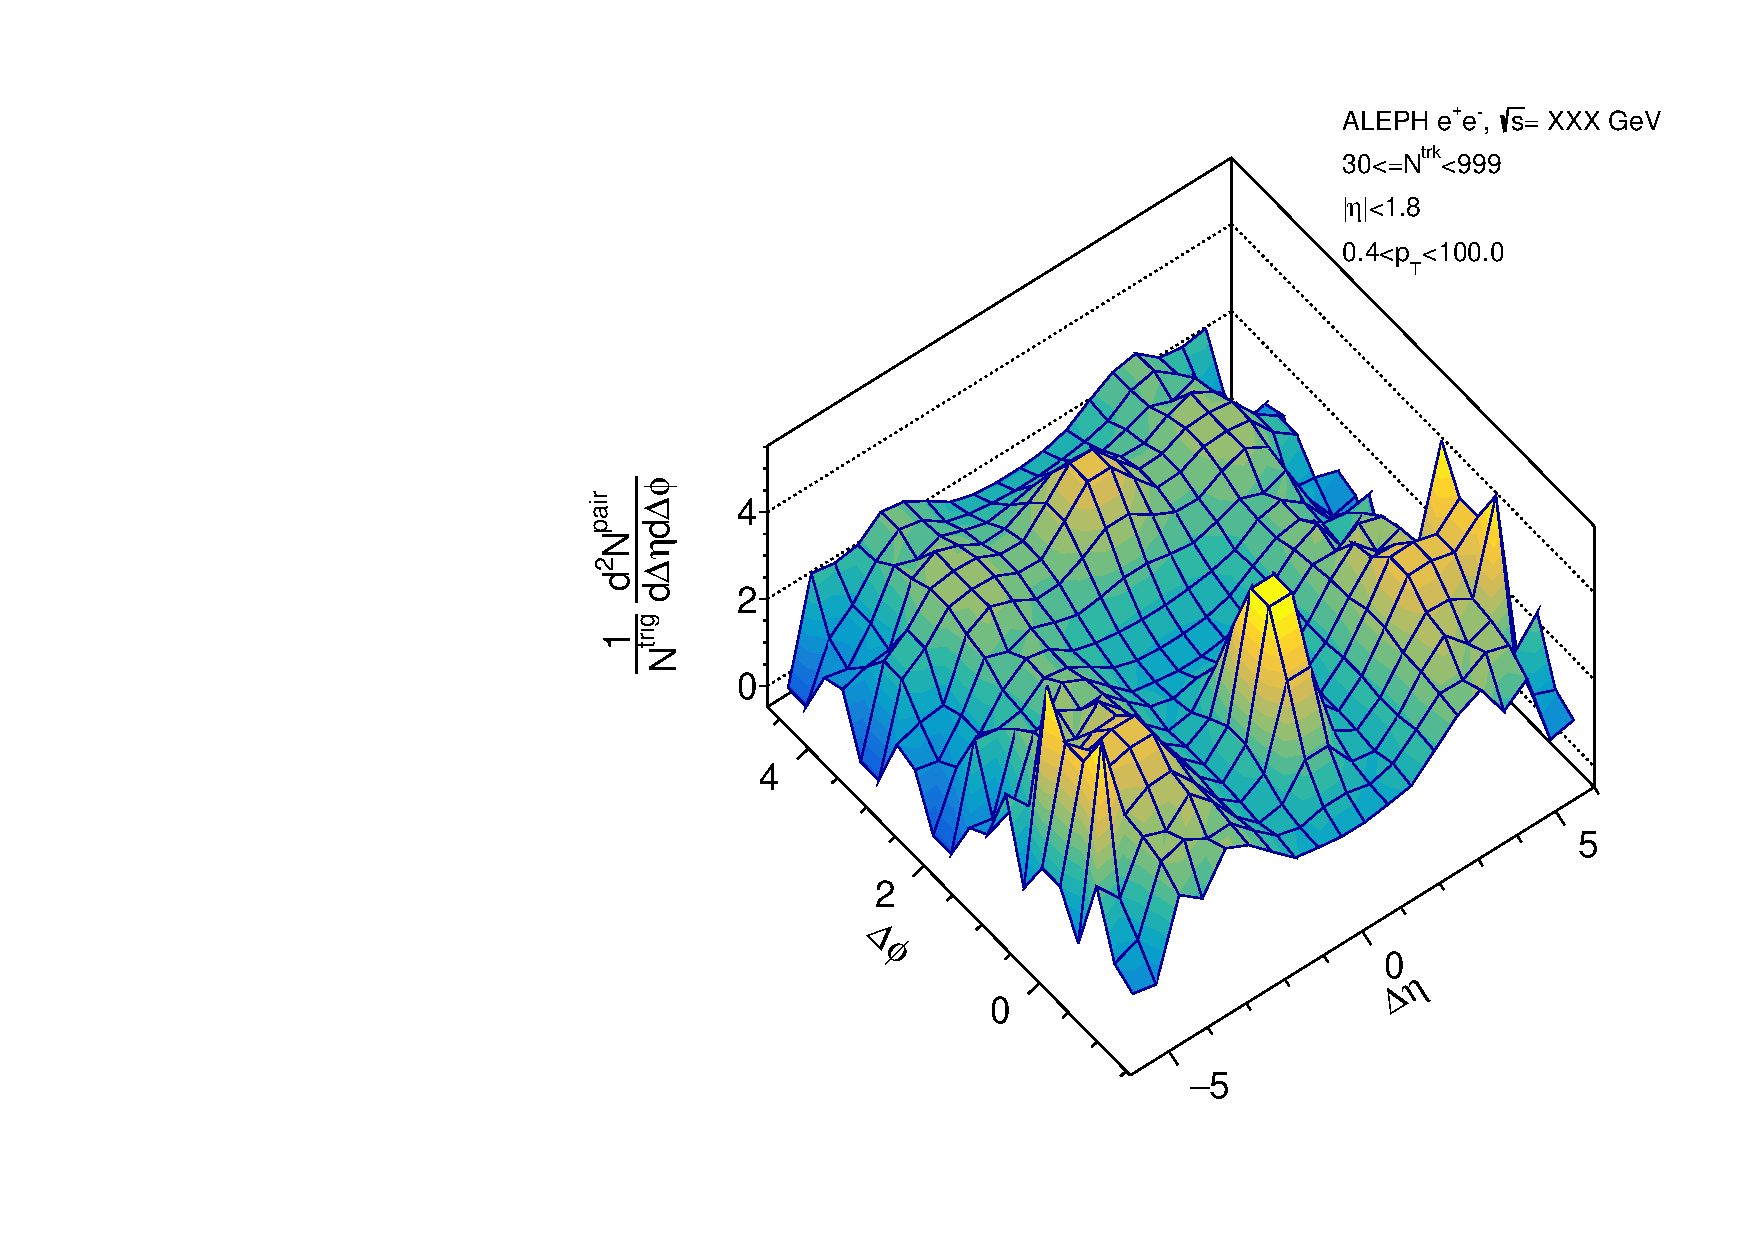
\includegraphics[width=\linewidth]{images/TwoParticleCorrelation/LEP1_THRUST/LEP1_THRUST_ratio1_30_999.pdf}
    \label{fig:LEP1 Thrust Axis, Ratio Plot, Multiplicity 30-999, Austin}
  \end{minipage}
  \hspace{0.0cm}
  \begin{minipage}[b]{0.32\linewidth}
    \centering
    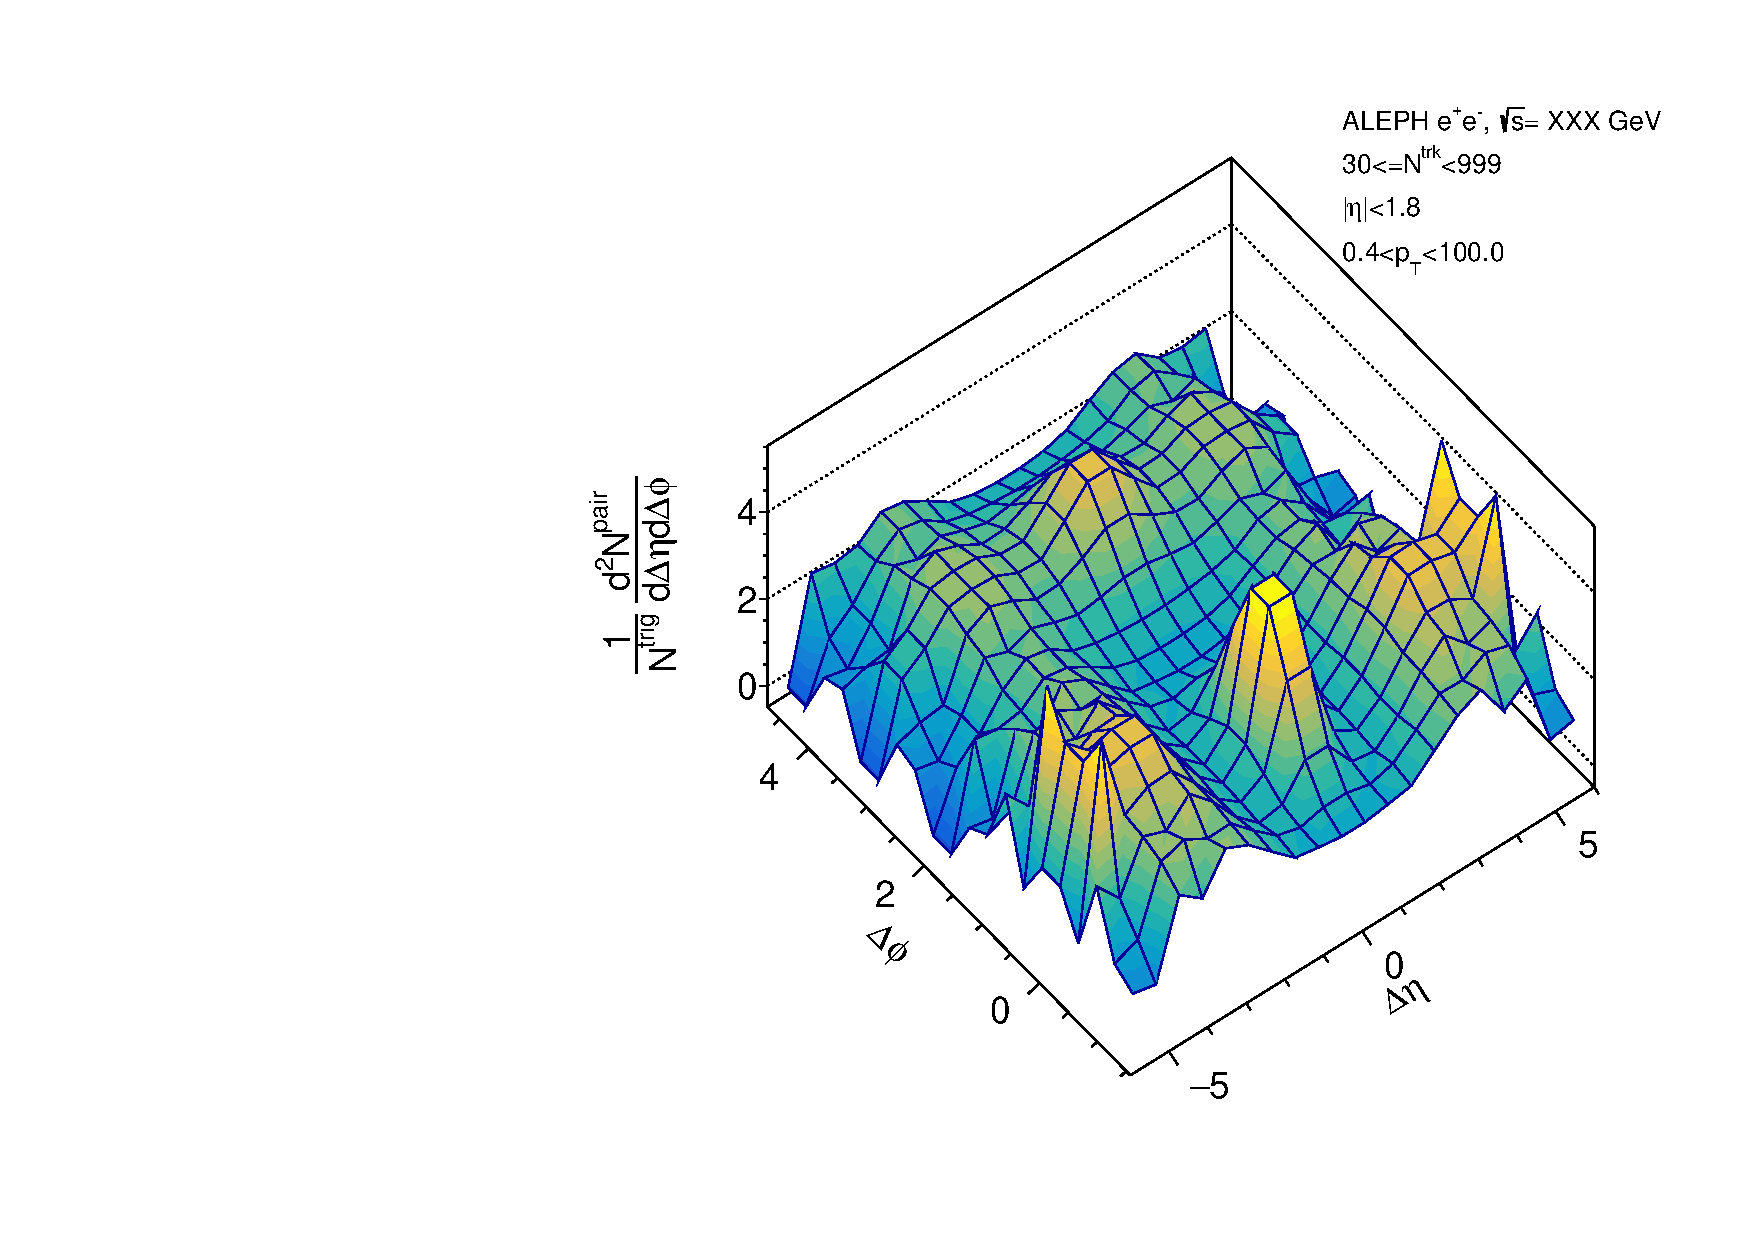
\includegraphics[width=\linewidth]{images/TwoParticleCorrelation/LEP1_THRUST/LEP1_THRUST_ratio2_30_999.pdf}
    \label{fig:LEP1 Thrust Axis, Ratio Plot, Multiplicity 30-999, Anthony}
  \end{minipage}
  \begin{minipage}[b]{0.32\linewidth}
    \centering
    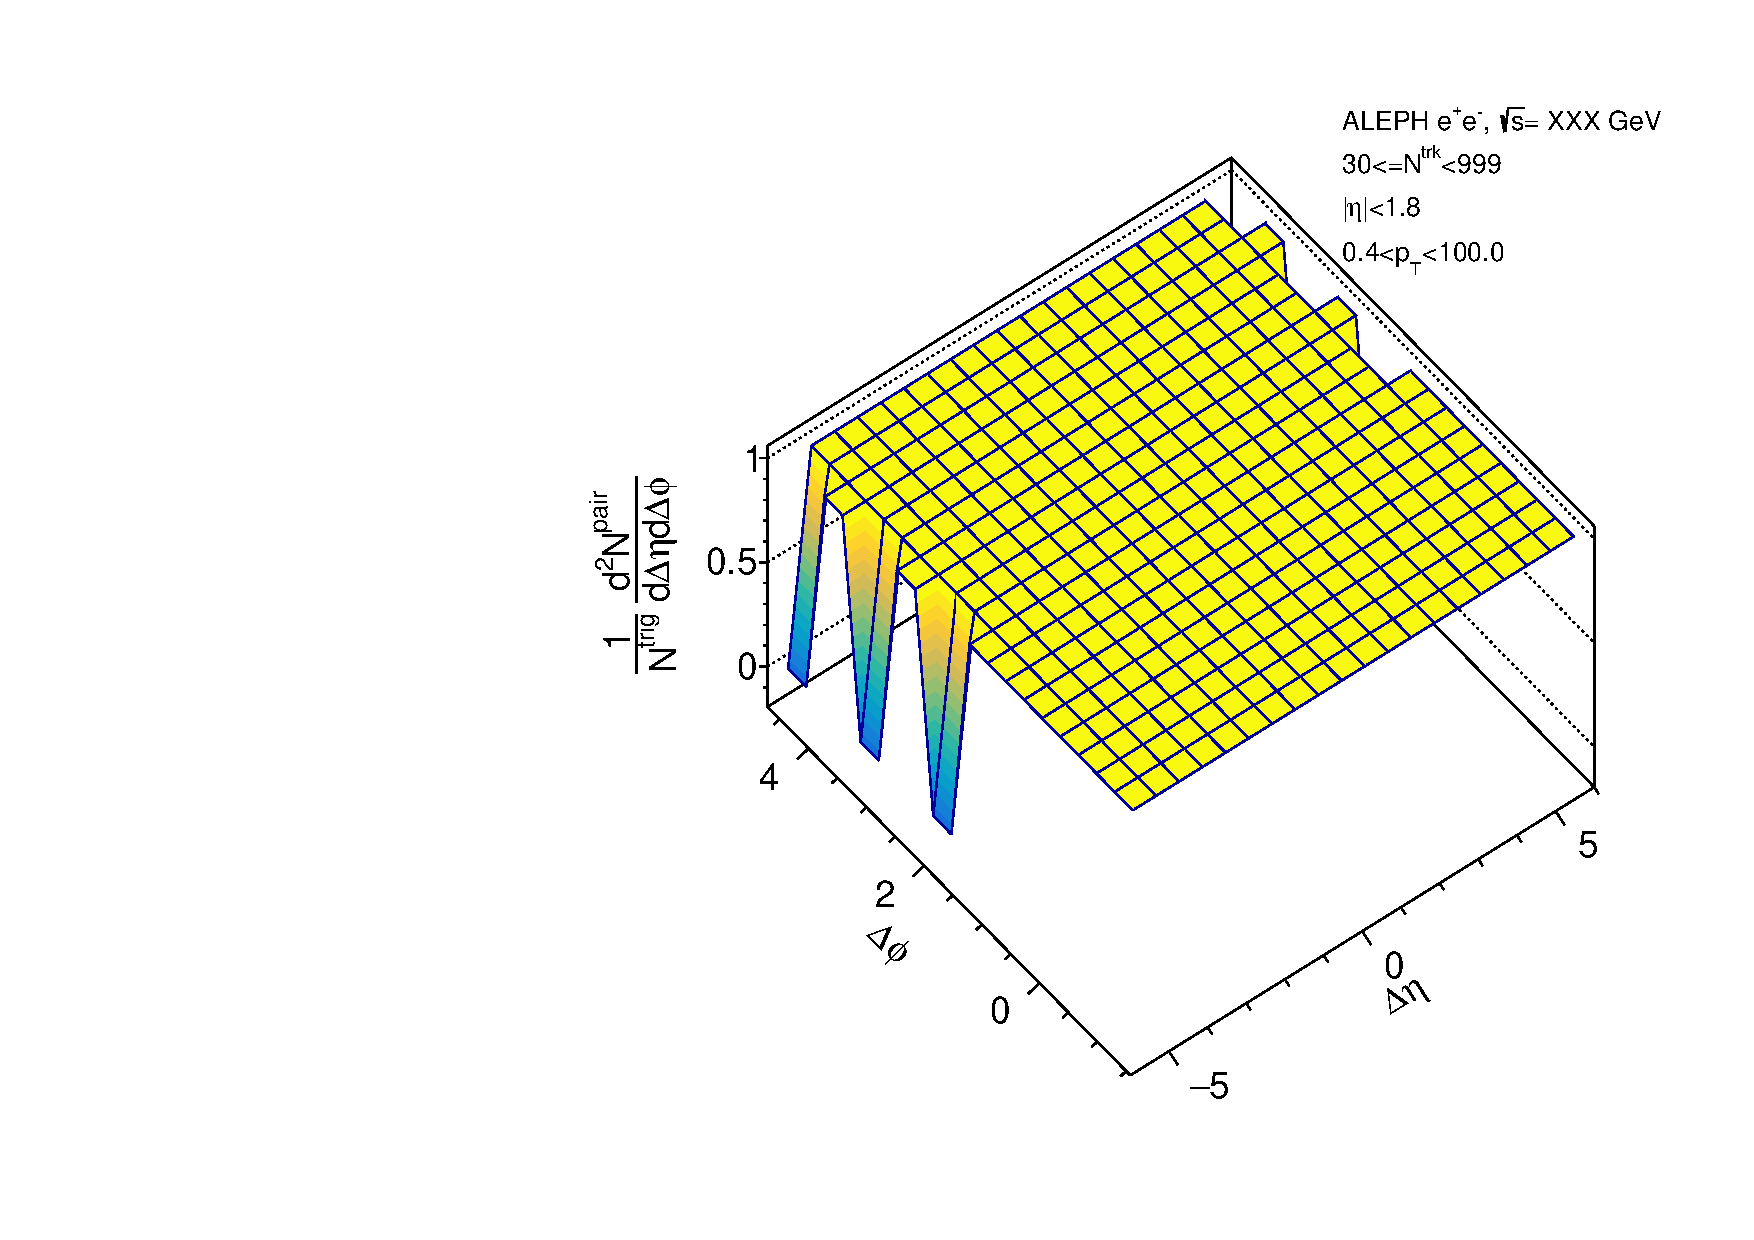
\includegraphics[width=\linewidth]{images/TwoParticleCorrelation/LEP1_THRUST/LEP1_THRUST_r_ratio_30_999.pdf}
    \label{fig:LEP1 Thrust Axis, Ratio Plot, Multiplicity 30-999, Ratio}
  \end{minipage}
\end{figure}

%%%%%%%%%%%%%%%%%%%%%%%%%%%%%%%%%%%%%%%%%%%%%%%%%%%%%%%%%%%%%%%% LEP2 BEAM AXIS %%%%%%%%%%%%%%%%%%%%%%%%%%%%%%%%%%%%%%%%%%%%%%%%%%%%%%%%%%%%%%%%
%%%%%%%%%%%%%%%%%%%%%%%%%%%%%%%% Multiplicity 0-20 %%%%%%%%%%%%%%%%%%%%%%%%%%%%%%%%
\begin{figure}[htbp]
  \caption{LEP2 Beam Axis, Ratio Plot, Multiplicity 0-20 (Austin, Anthony, Ratio)}
  \begin{minipage}[b]{0.32\linewidth}
    \centering
    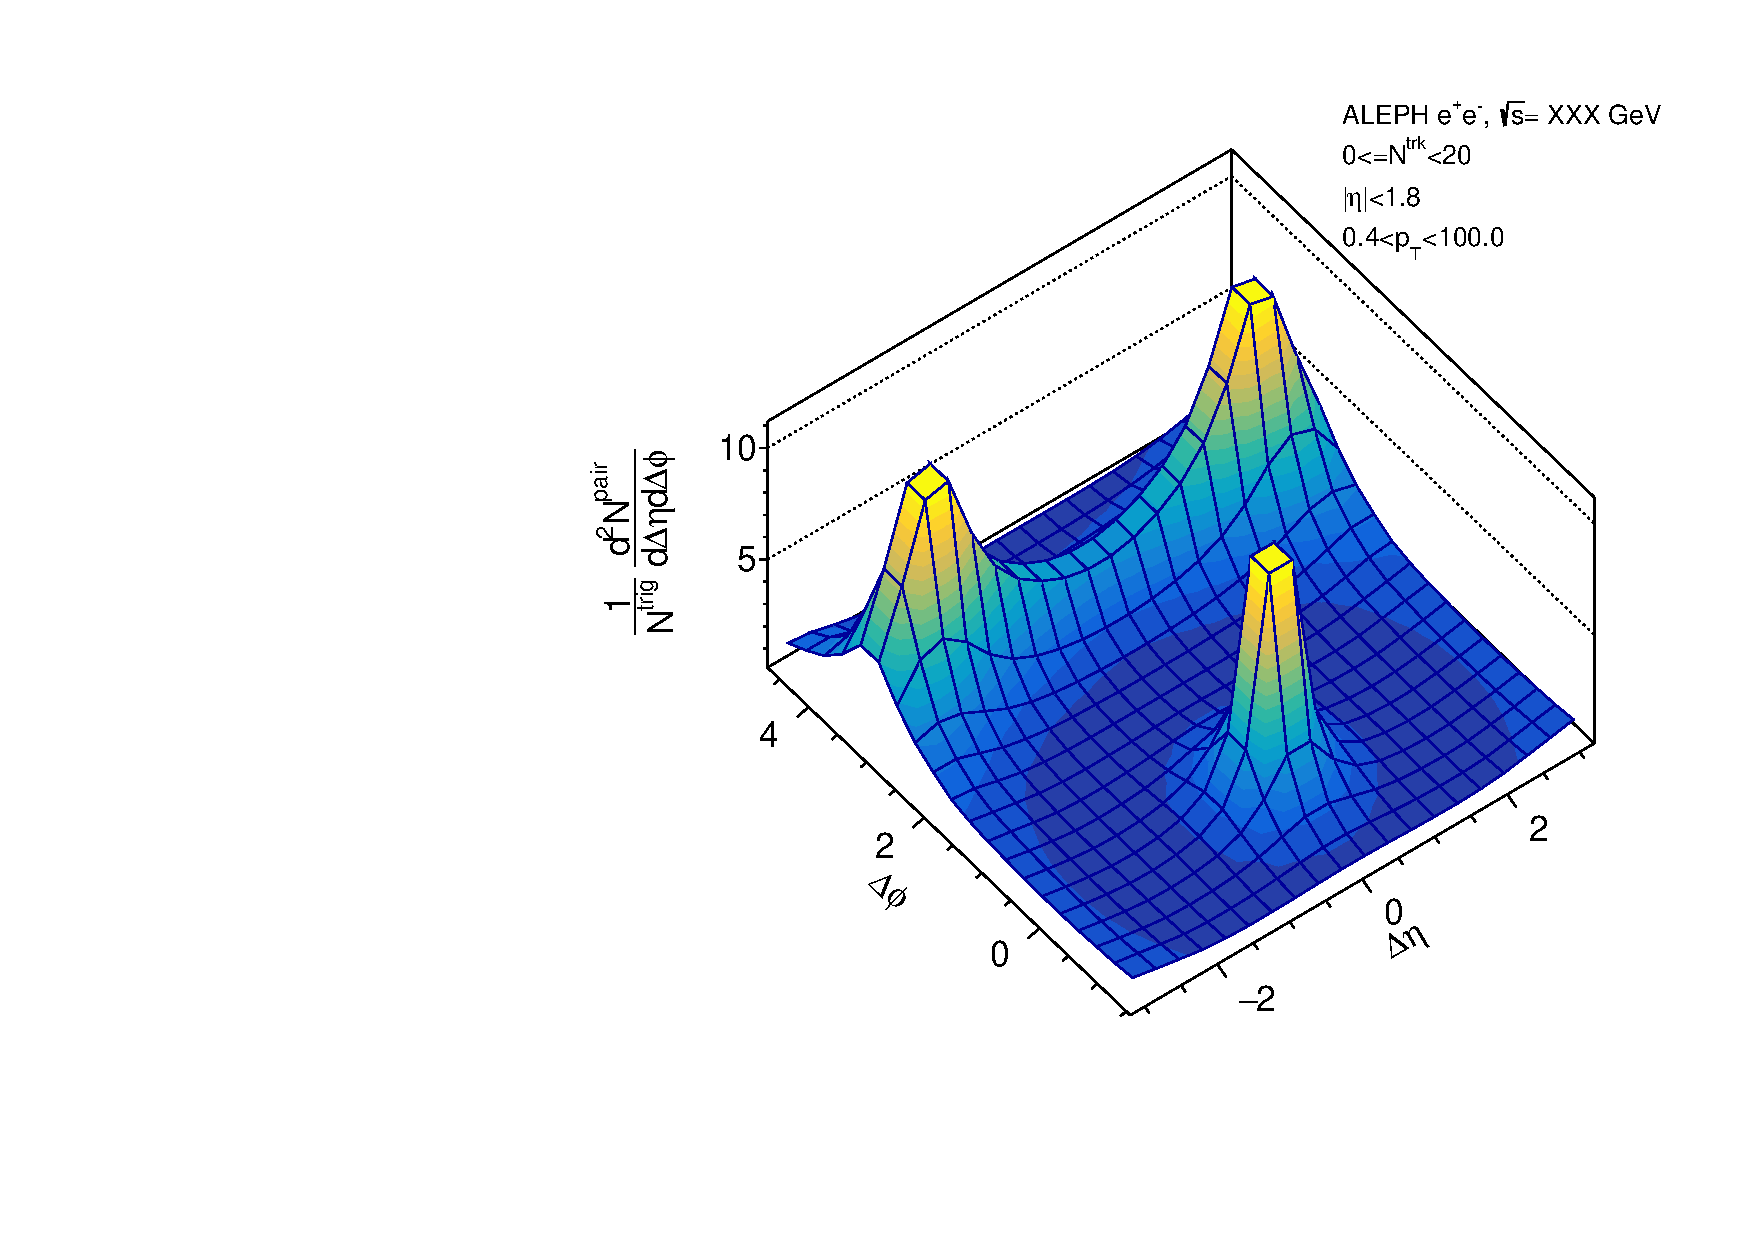
\includegraphics[width=\linewidth]{images/TwoParticleCorrelation/LEP2_BEAM/LEP2_BEAM_ratio1_0_20.pdf}
    \label{fig:LEP2 Beam Axis, Ratio Plot, Multiplicity 0-20, Austin}
  \end{minipage}
  \hspace{0.0cm}
  \begin{minipage}[b]{0.32\linewidth}
    \centering
    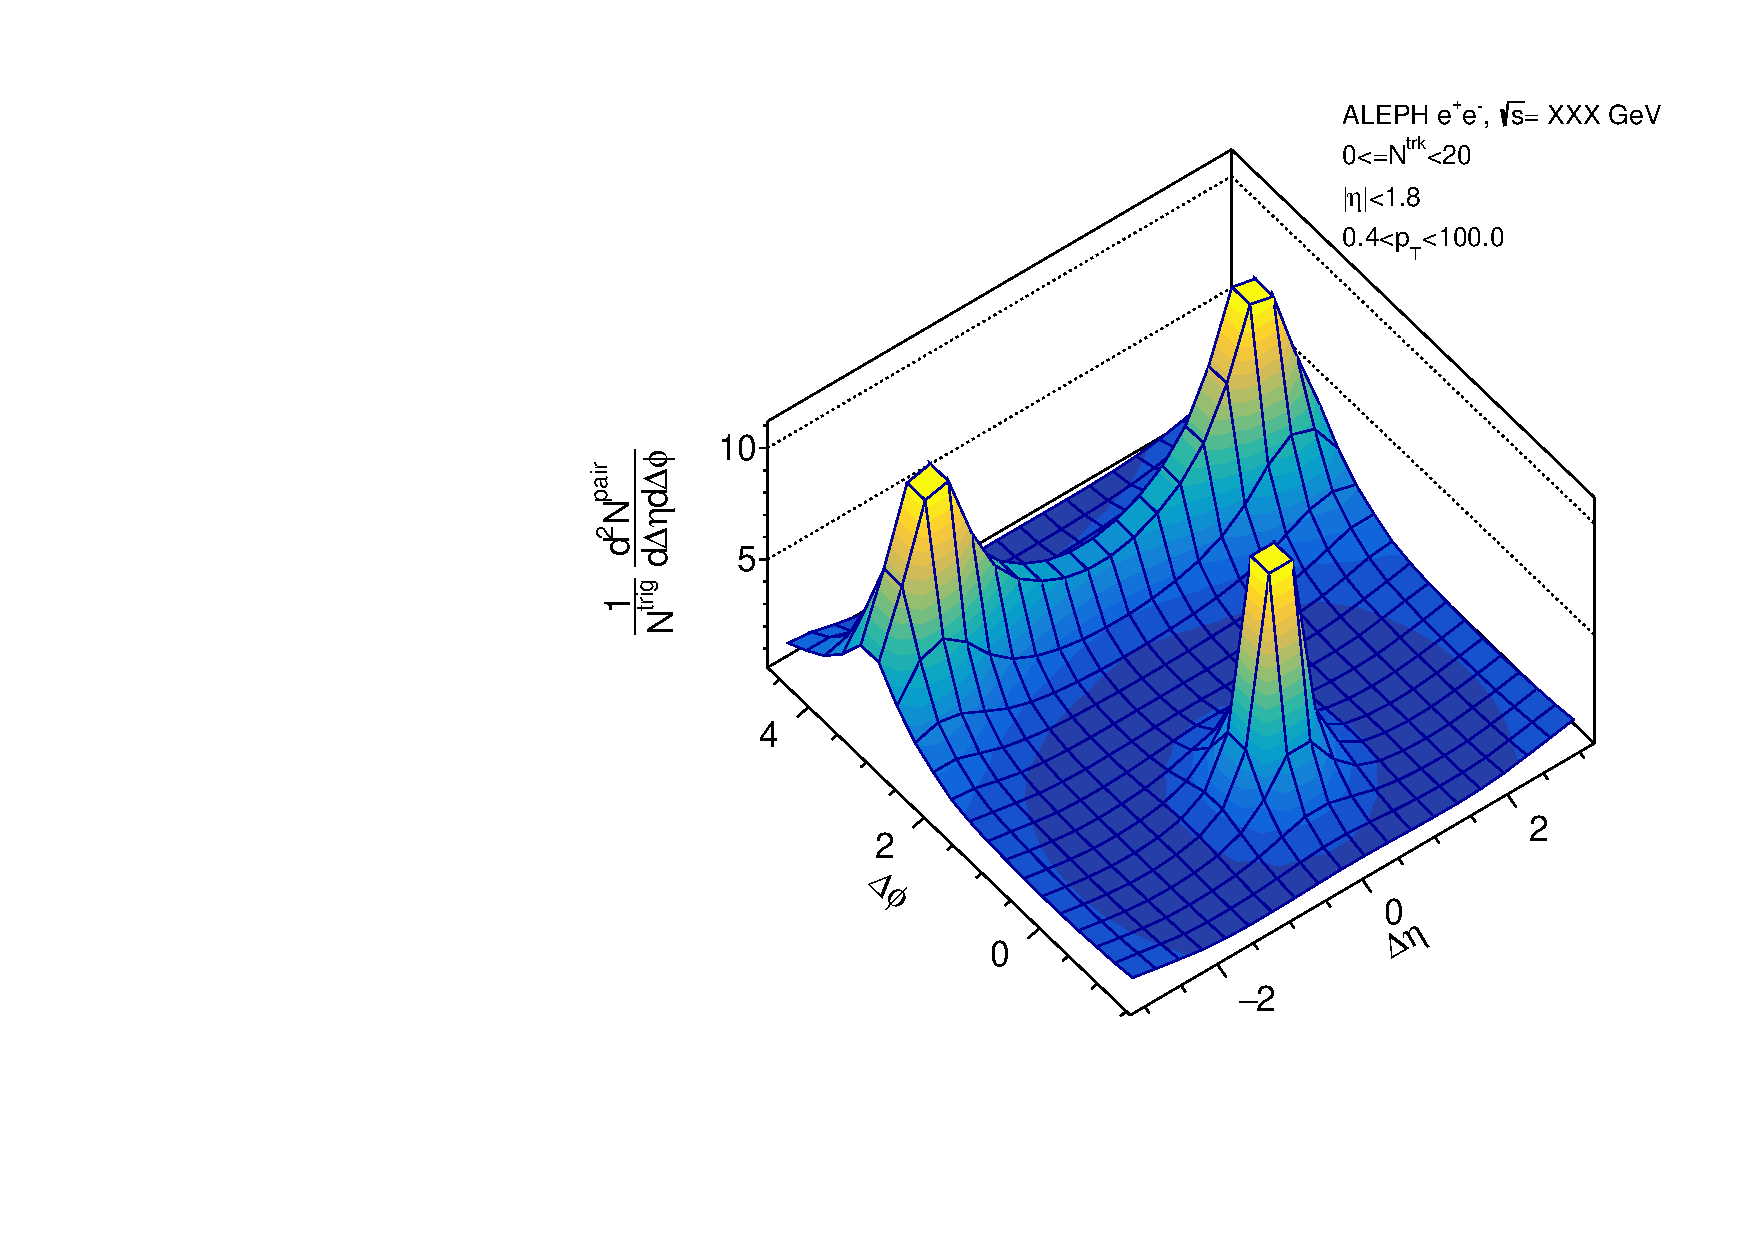
\includegraphics[width=\linewidth]{images/TwoParticleCorrelation/LEP2_BEAM/LEP2_BEAM_ratio2_0_20.pdf}
    \label{fig:LEP2 Beam Axis, Ratio Plot, Multiplicity 0-20, Anthony}
  \end{minipage}
  \begin{minipage}[b]{0.32\linewidth}
    \centering
    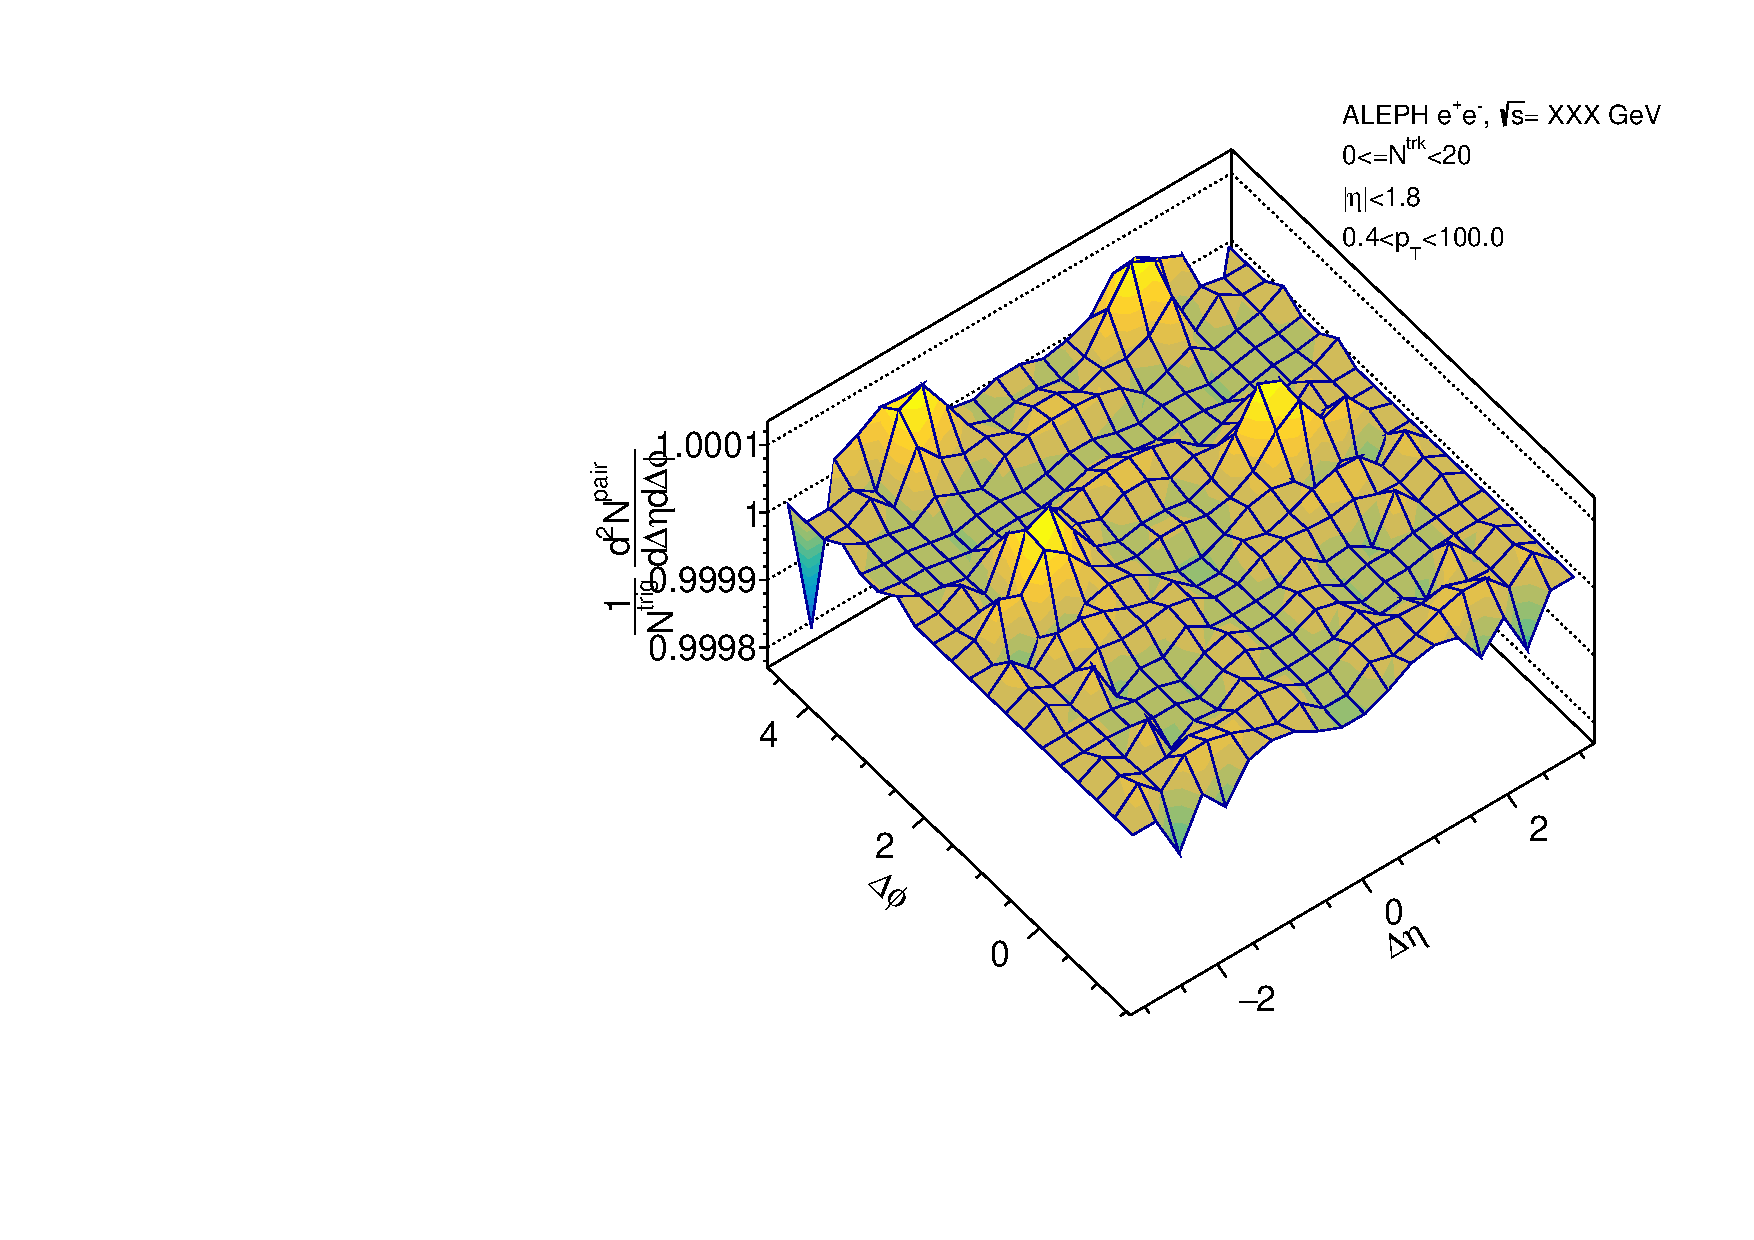
\includegraphics[width=\linewidth]{images/TwoParticleCorrelation/LEP2_BEAM/LEP2_BEAM_r_ratio_0_20.pdf}
    \label{fig:LEP2 Beam Axis, Ratio Plot, Multiplicity 0-20, Ratio}
  \end{minipage}
\end{figure}


%%%%%%%%%%%%%%%%%%%%%%%%%%%%%%%% Multiplicity 20-30 %%%%%%%%%%%%%%%%%%%%%%%%%%%%%%%%
\begin{figure}[htbp]
  \caption{LEP2 Beam Axis, Ratio Plot, Multiplicity 20-30 (Austin, Anthony, Ratio)}
  \begin{minipage}[b]{0.32\linewidth}
    \centering
    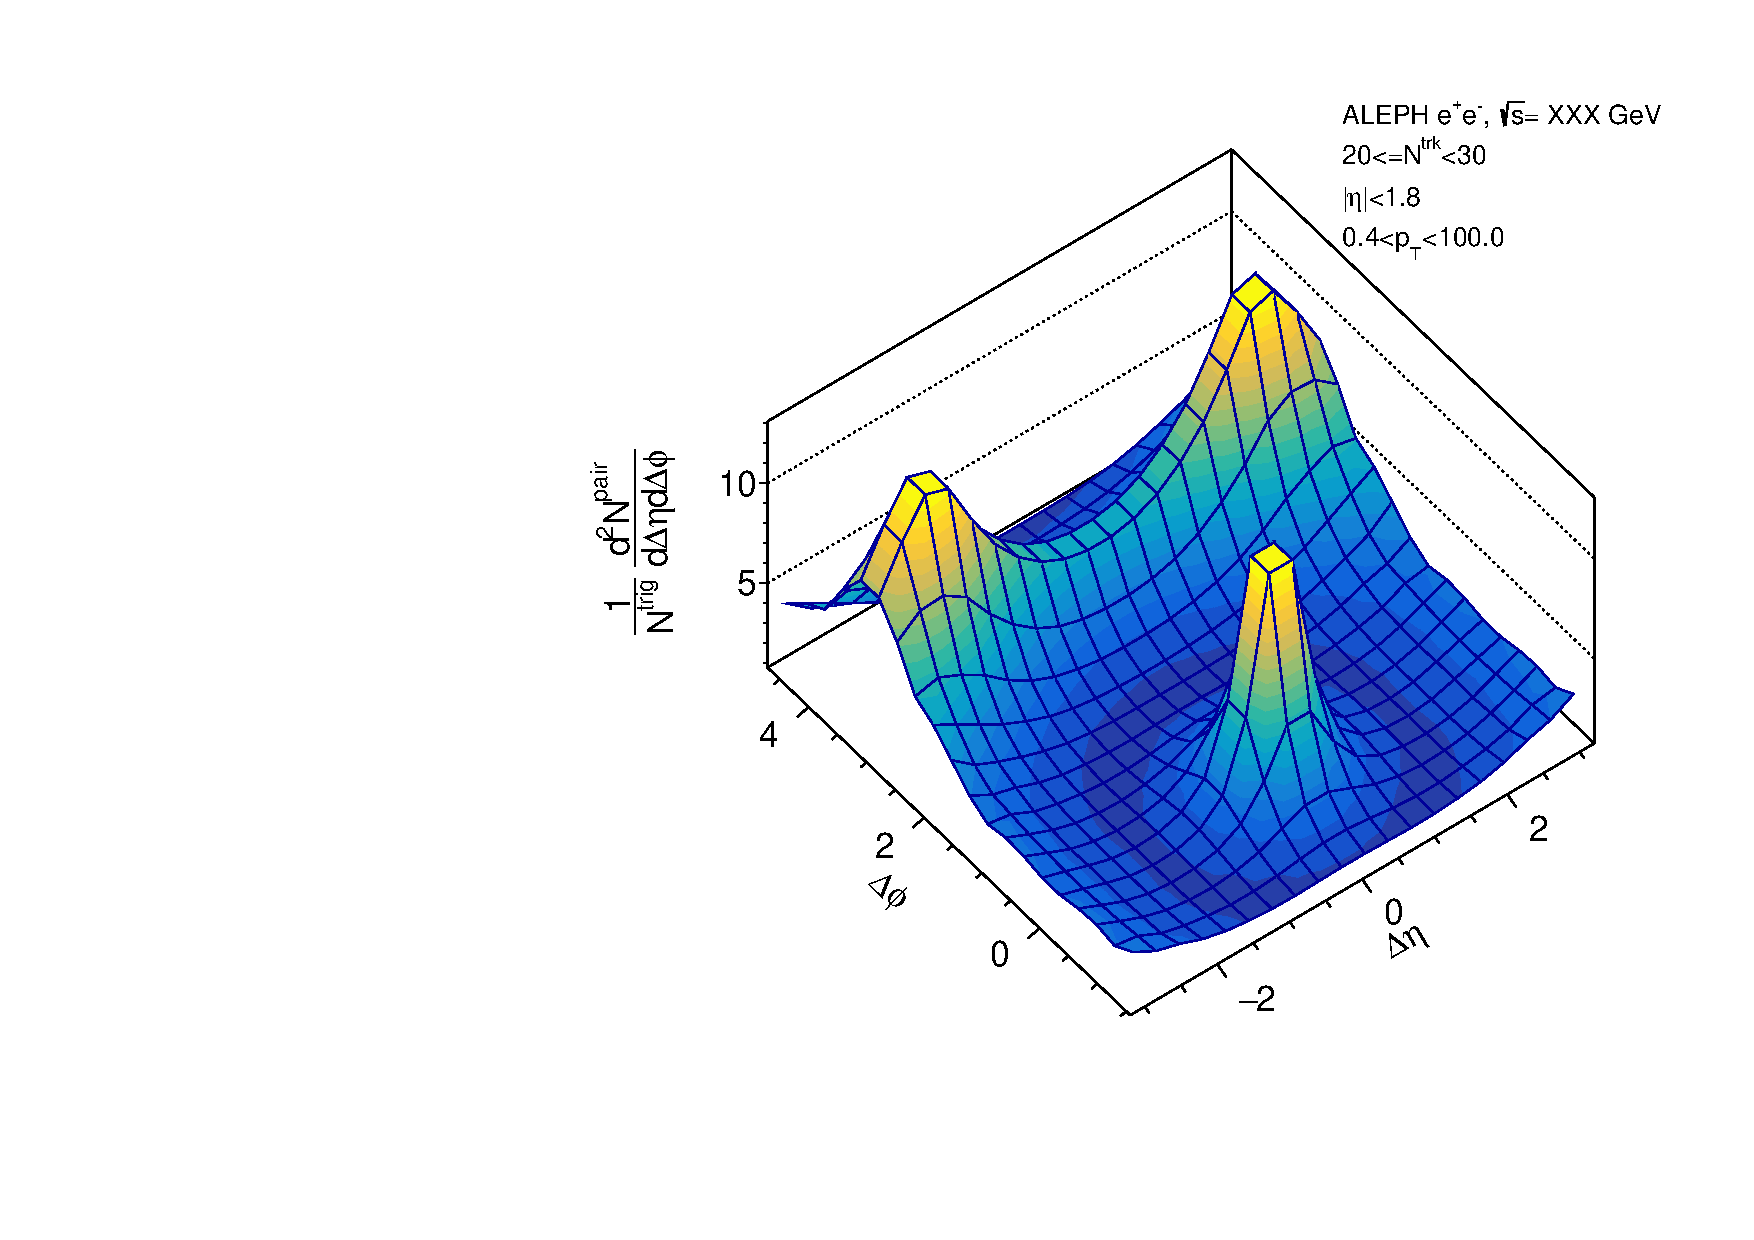
\includegraphics[width=\linewidth]{images/TwoParticleCorrelation/LEP2_BEAM/LEP2_BEAM_ratio1_20_30.pdf}
    \label{fig:LEP2 Beam Axis, Ratio Plot, Multiplicity 20-30, Austin}
  \end{minipage}
  \hspace{0.0cm}
  \begin{minipage}[b]{0.32\linewidth}
    \centering
    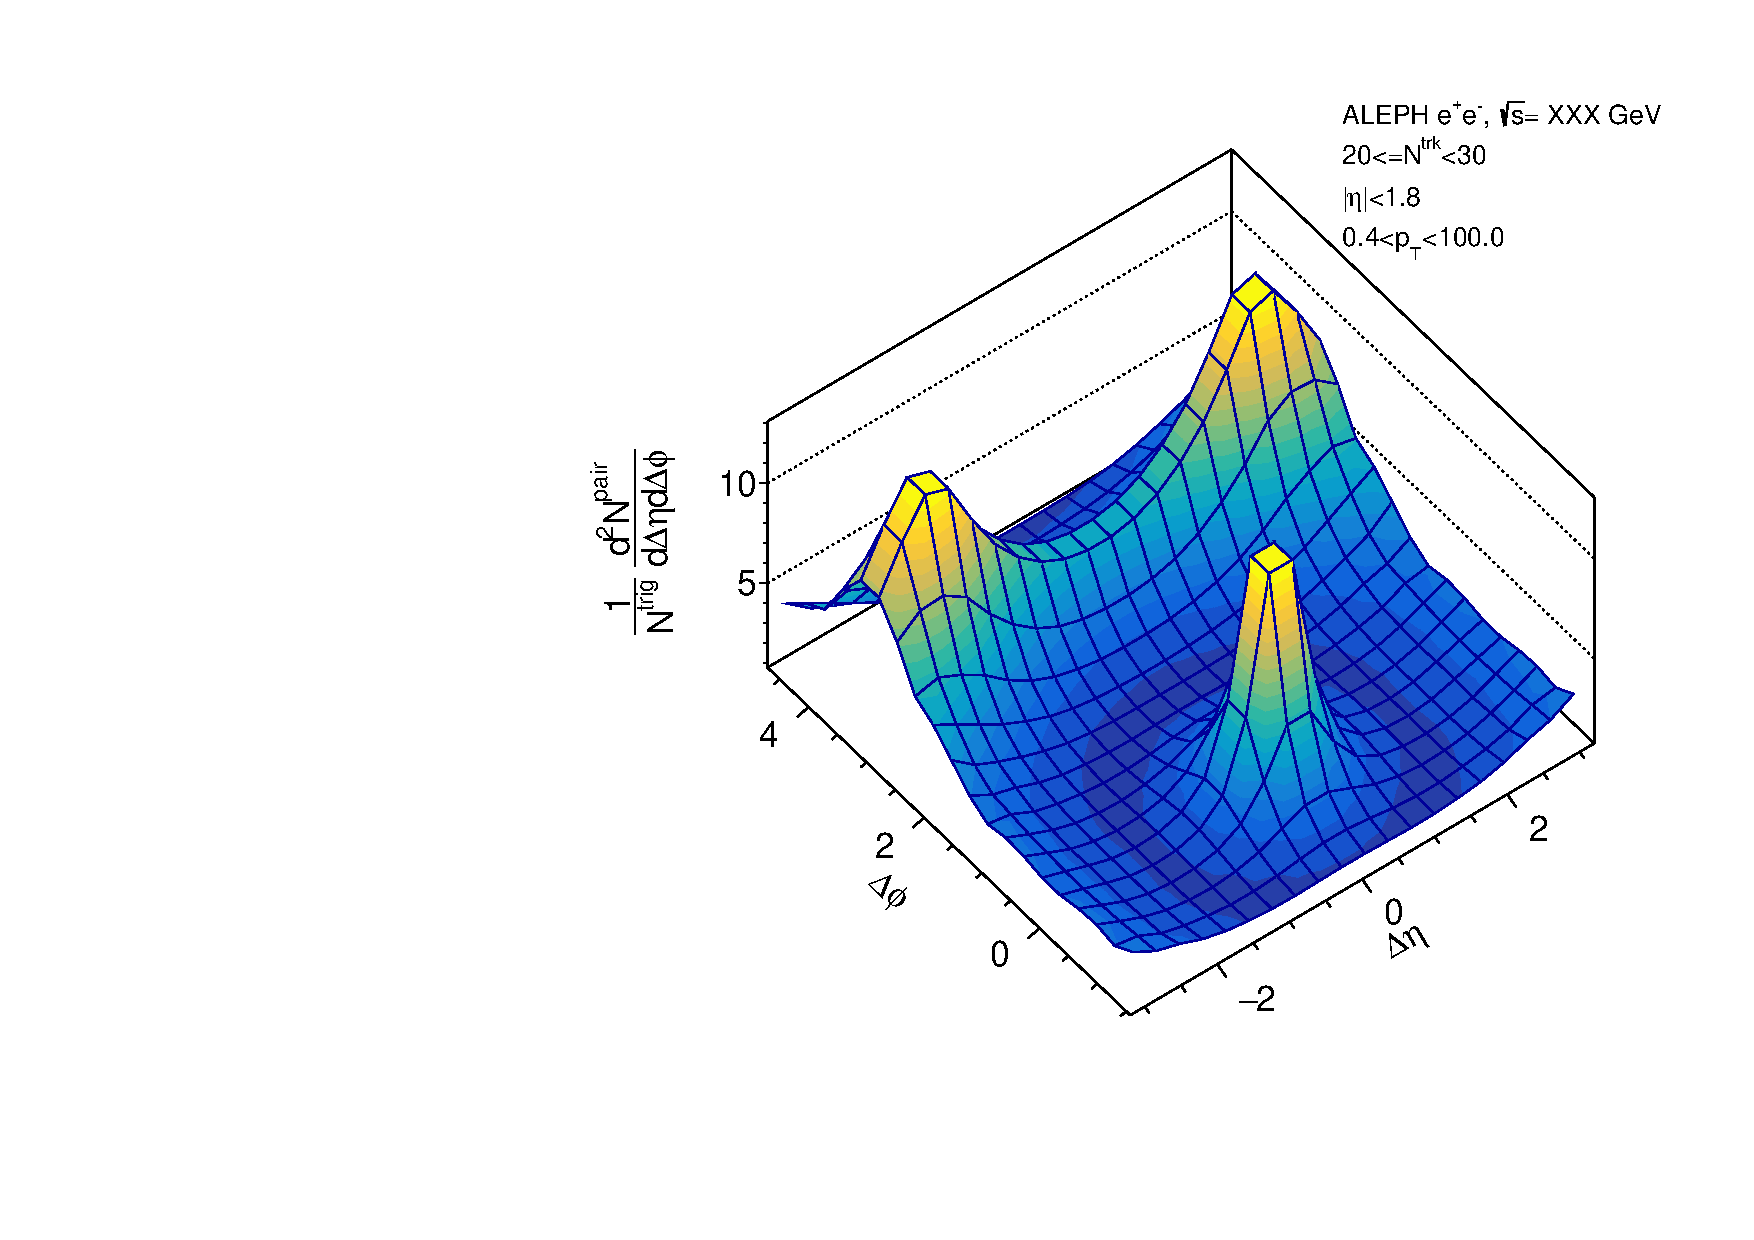
\includegraphics[width=\linewidth]{images/TwoParticleCorrelation/LEP2_BEAM/LEP2_BEAM_ratio2_20_30.pdf}
    \label{fig:LEP2 Beam Axis, Ratio Plot, Multiplicity 20-30, Anthony}
  \end{minipage}
  \begin{minipage}[b]{0.32\linewidth}
    \centering
    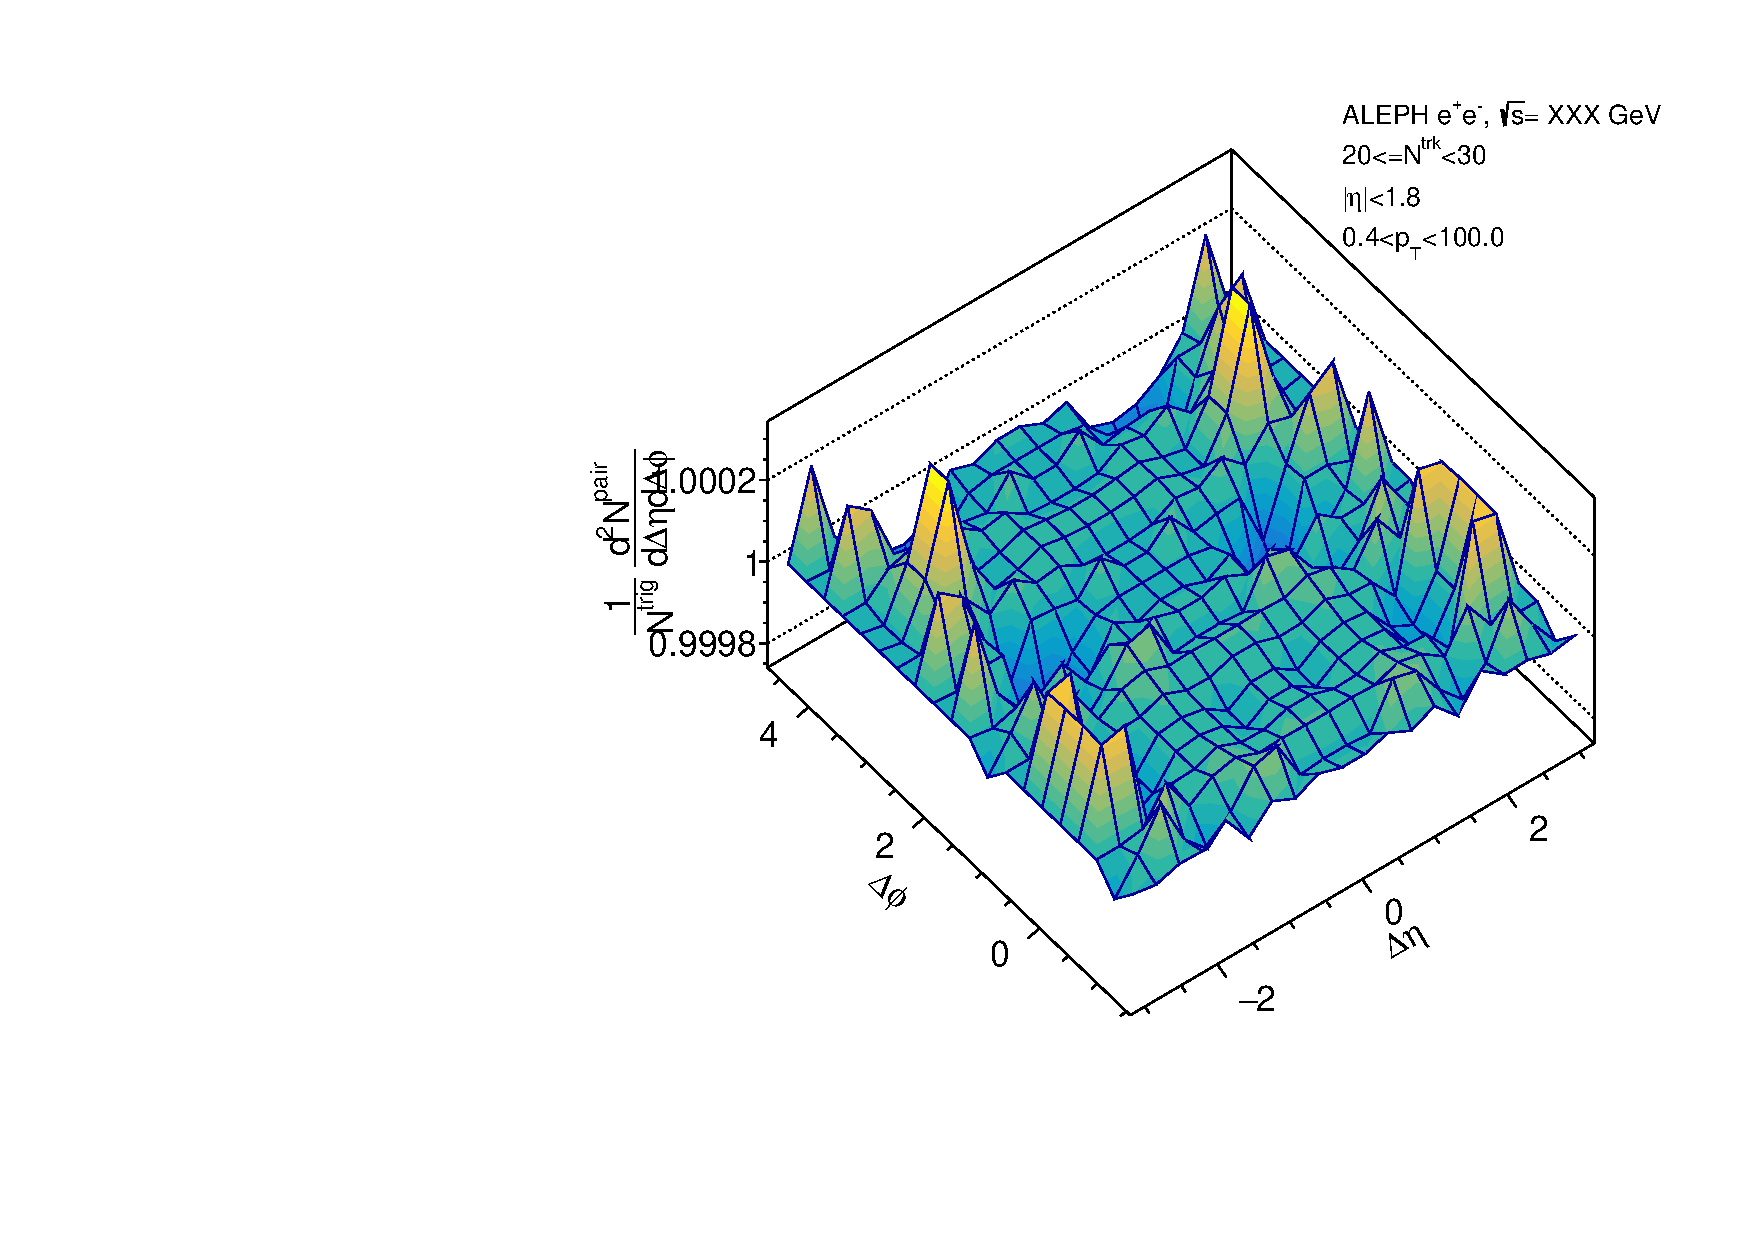
\includegraphics[width=\linewidth]{images/TwoParticleCorrelation/LEP2_BEAM/LEP2_BEAM_r_ratio_20_30.pdf}
    \label{fig:LEP2 Beam Axis, Ratio Plot, Multiplicity 20-30, Ratio}
  \end{minipage}
\end{figure}

%%%%%%%%%%%%%%%%%%%%%%%%%%%%%%%% Multiplicity 30-999 %%%%%%%%%%%%%%%%%%%%%%%%%%%%%%%%
\begin{figure}[htbp]
  \caption{LEP2 Beam Axis, Ratio Plot, Multiplicity 30-999 (Austin, Anthony, Ratio)}
  \begin{minipage}[b]{0.32\linewidth}
    \centering
    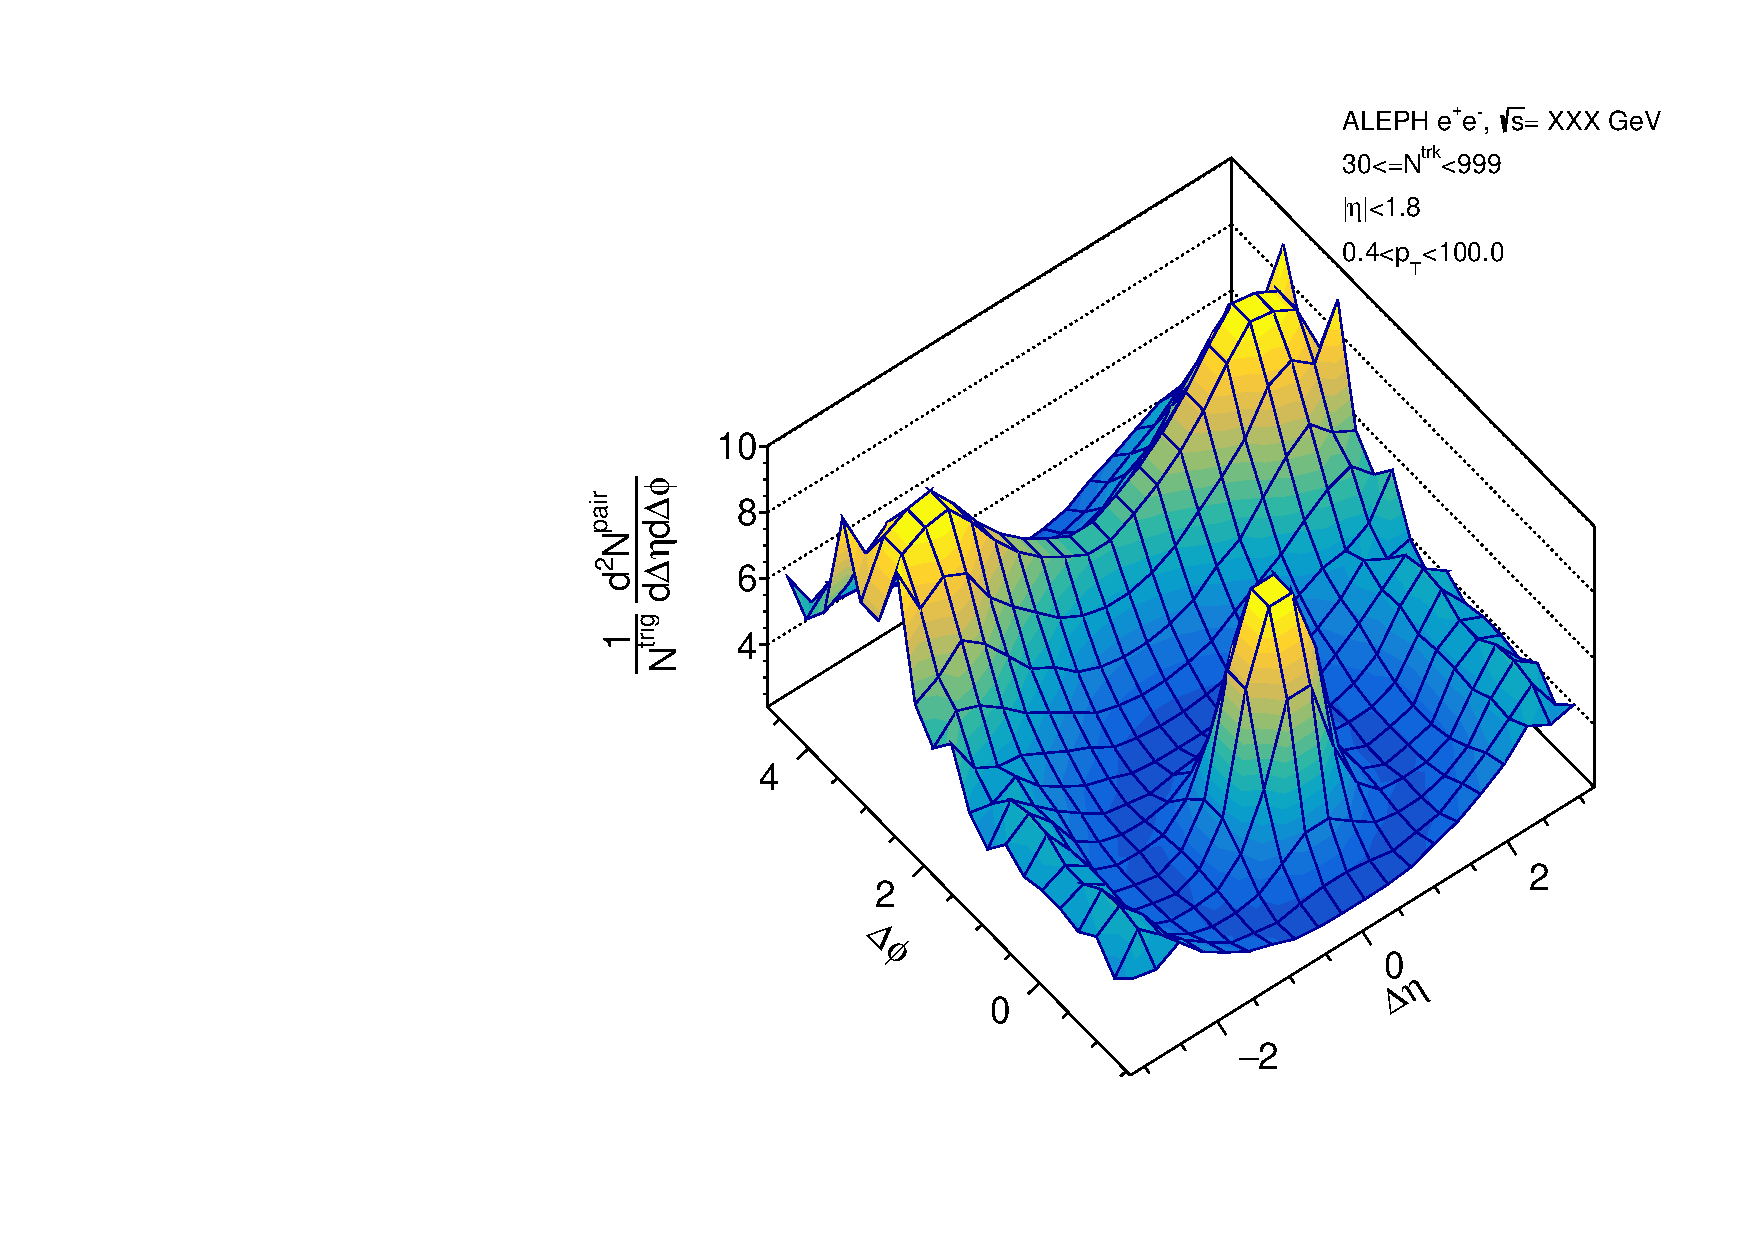
\includegraphics[width=\linewidth]{images/TwoParticleCorrelation/LEP2_BEAM/LEP2_BEAM_ratio1_30_999.pdf}
    \label{fig:LEP2 Beam Axis, Ratio Plot, Multiplicity 30-999, Austin}
  \end{minipage}
  \hspace{0.0cm}
  \begin{minipage}[b]{0.32\linewidth}
    \centering
    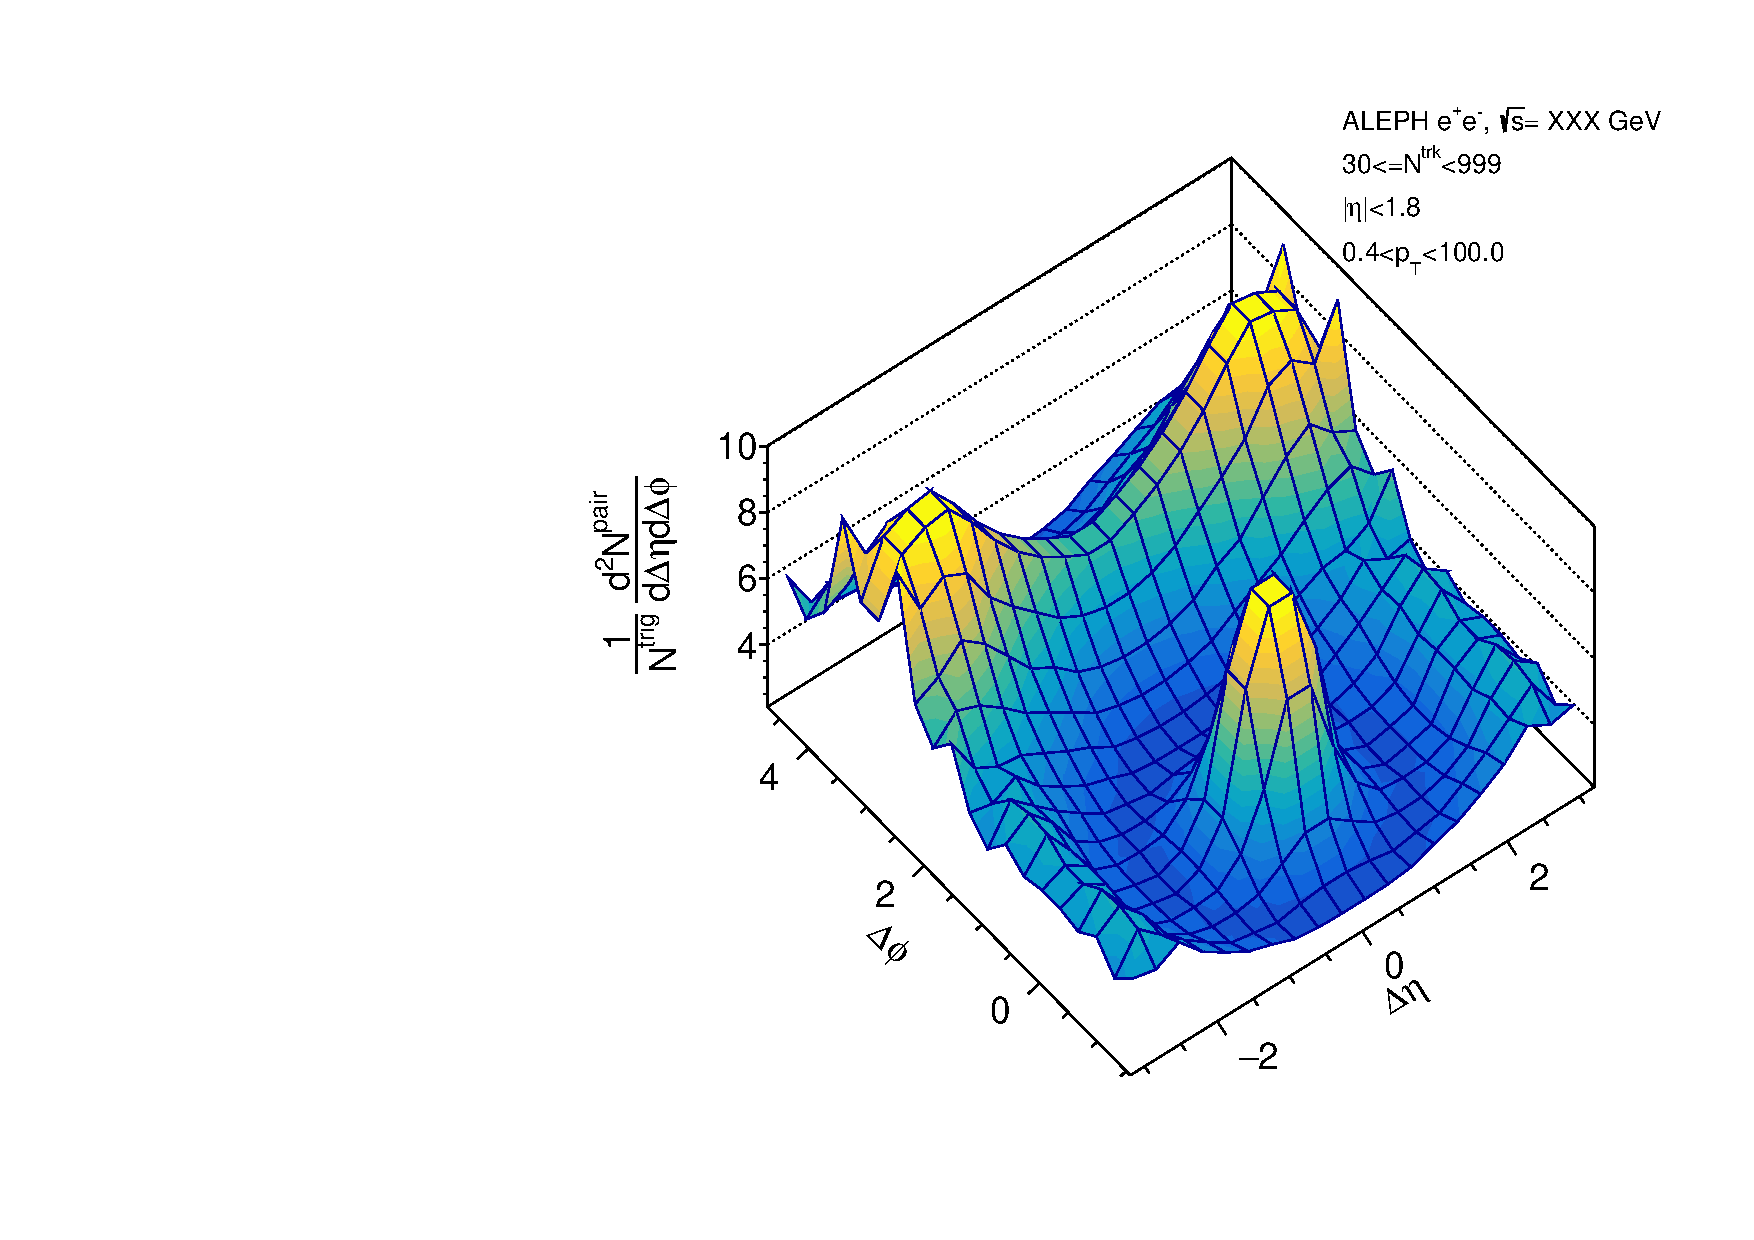
\includegraphics[width=\linewidth]{images/TwoParticleCorrelation/LEP2_BEAM/LEP2_BEAM_ratio2_30_999.pdf}
    \label{fig:LEP2 Beam Axis, Ratio Plot, Multiplicity 30-999, Anthony}
  \end{minipage}
  \begin{minipage}[b]{0.32\linewidth}
    \centering
    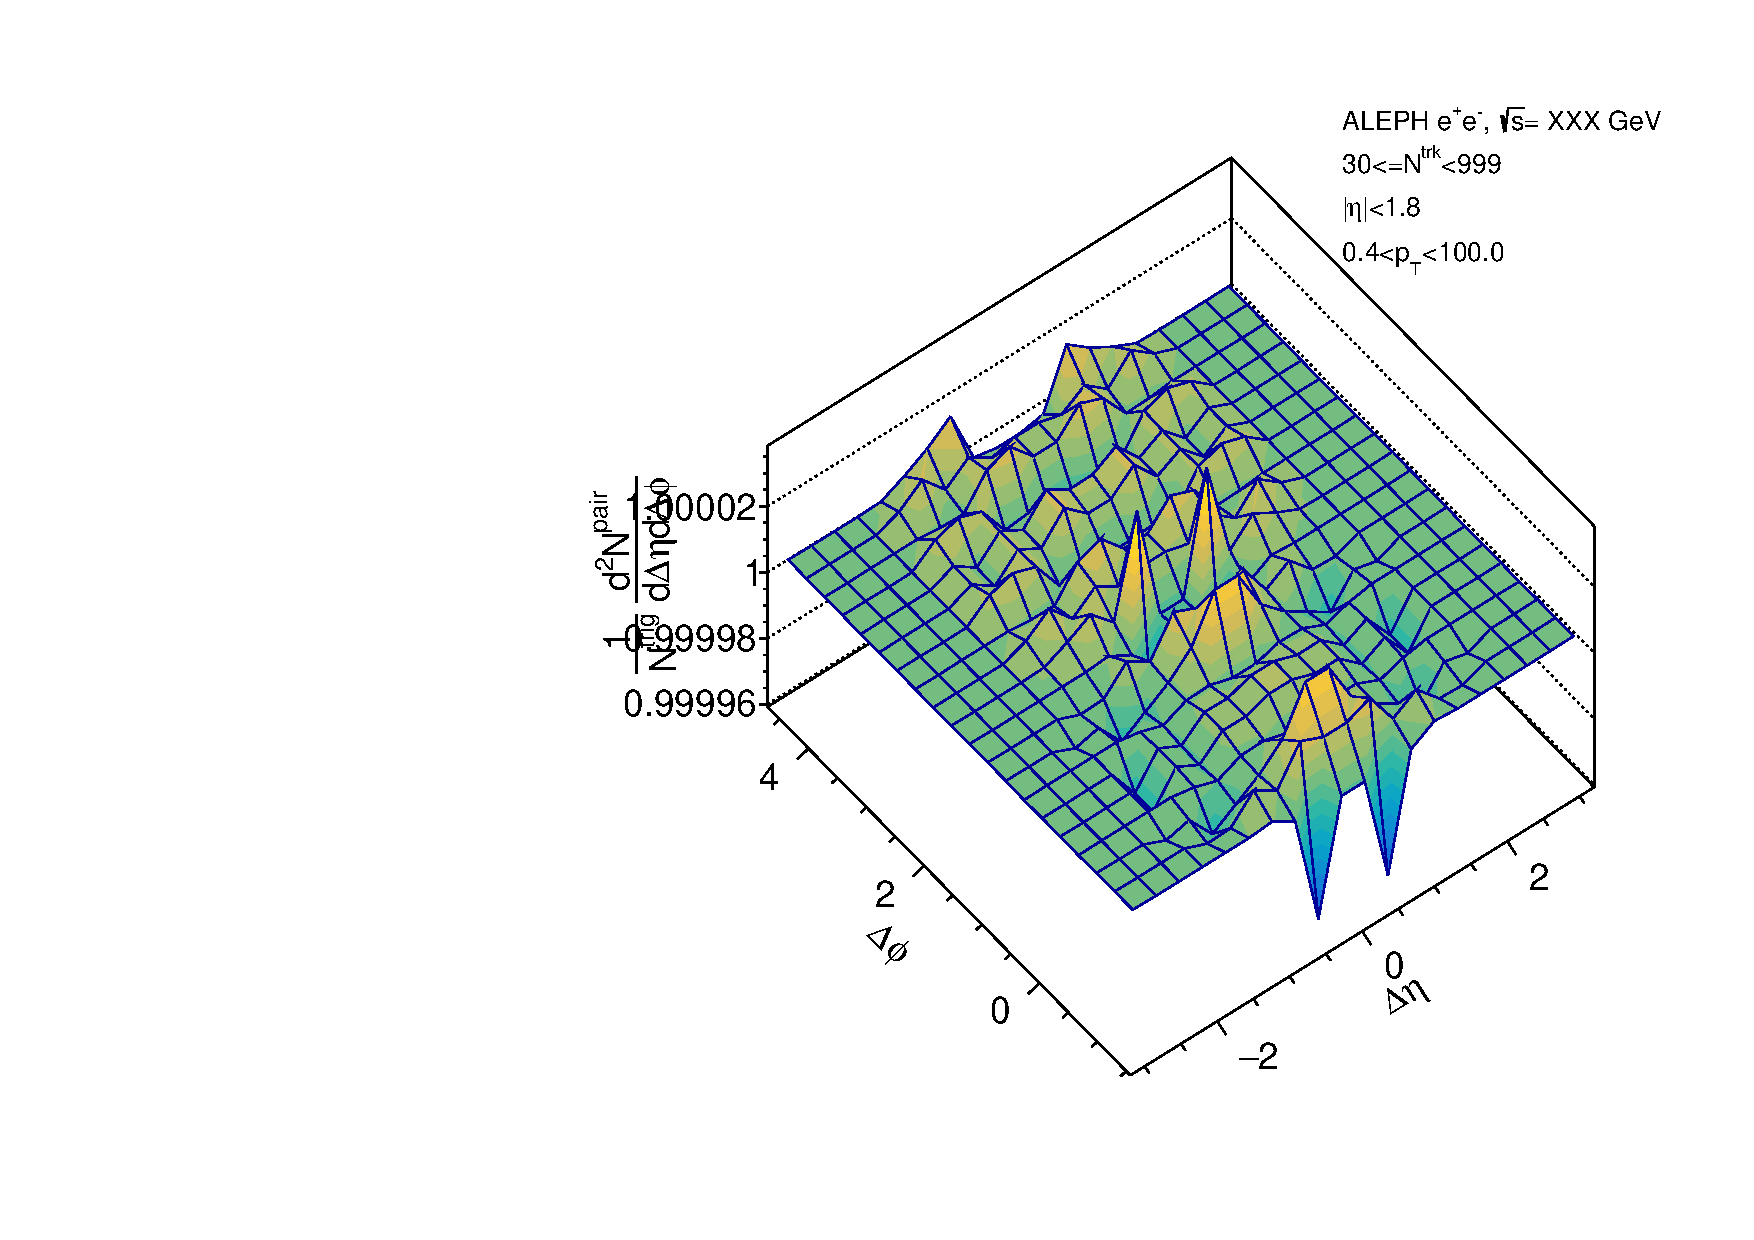
\includegraphics[width=\linewidth]{images/TwoParticleCorrelation/LEP2_BEAM/LEP2_BEAM_r_ratio_30_999.pdf}
    \label{fig:LEP2 Beam Axis, Ratio Plot, Multiplicity 30-999, Ratio}
  \end{minipage}
\end{figure}

%%%%%%%%%%%%%%%%%%%%%%%%%%%%%%%%%%%%%%%%%%%%%%%%%%%%%%%%%%%%%%%% LEP2 THRUST AXIS %%%%%%%%%%%%%%%%%%%%%%%%%%%%%%%%%%%%%%%%%%%%%%%%%%%%%%%%%%%%%%%%
%%%%%%%%%%%%%%%%%%%%%%%%%%%%%%%% Multiplicity 0-20 %%%%%%%%%%%%%%%%%%%%%%%%%%%%%%%%
\begin{figure}[htbp]
  \caption{LEP2 Thrust Axis, Ratio Plot, Multiplicity 0-20 (Austin, Anthony, Ratio)}
  \begin{minipage}[b]{0.32\linewidth}
    \centering
    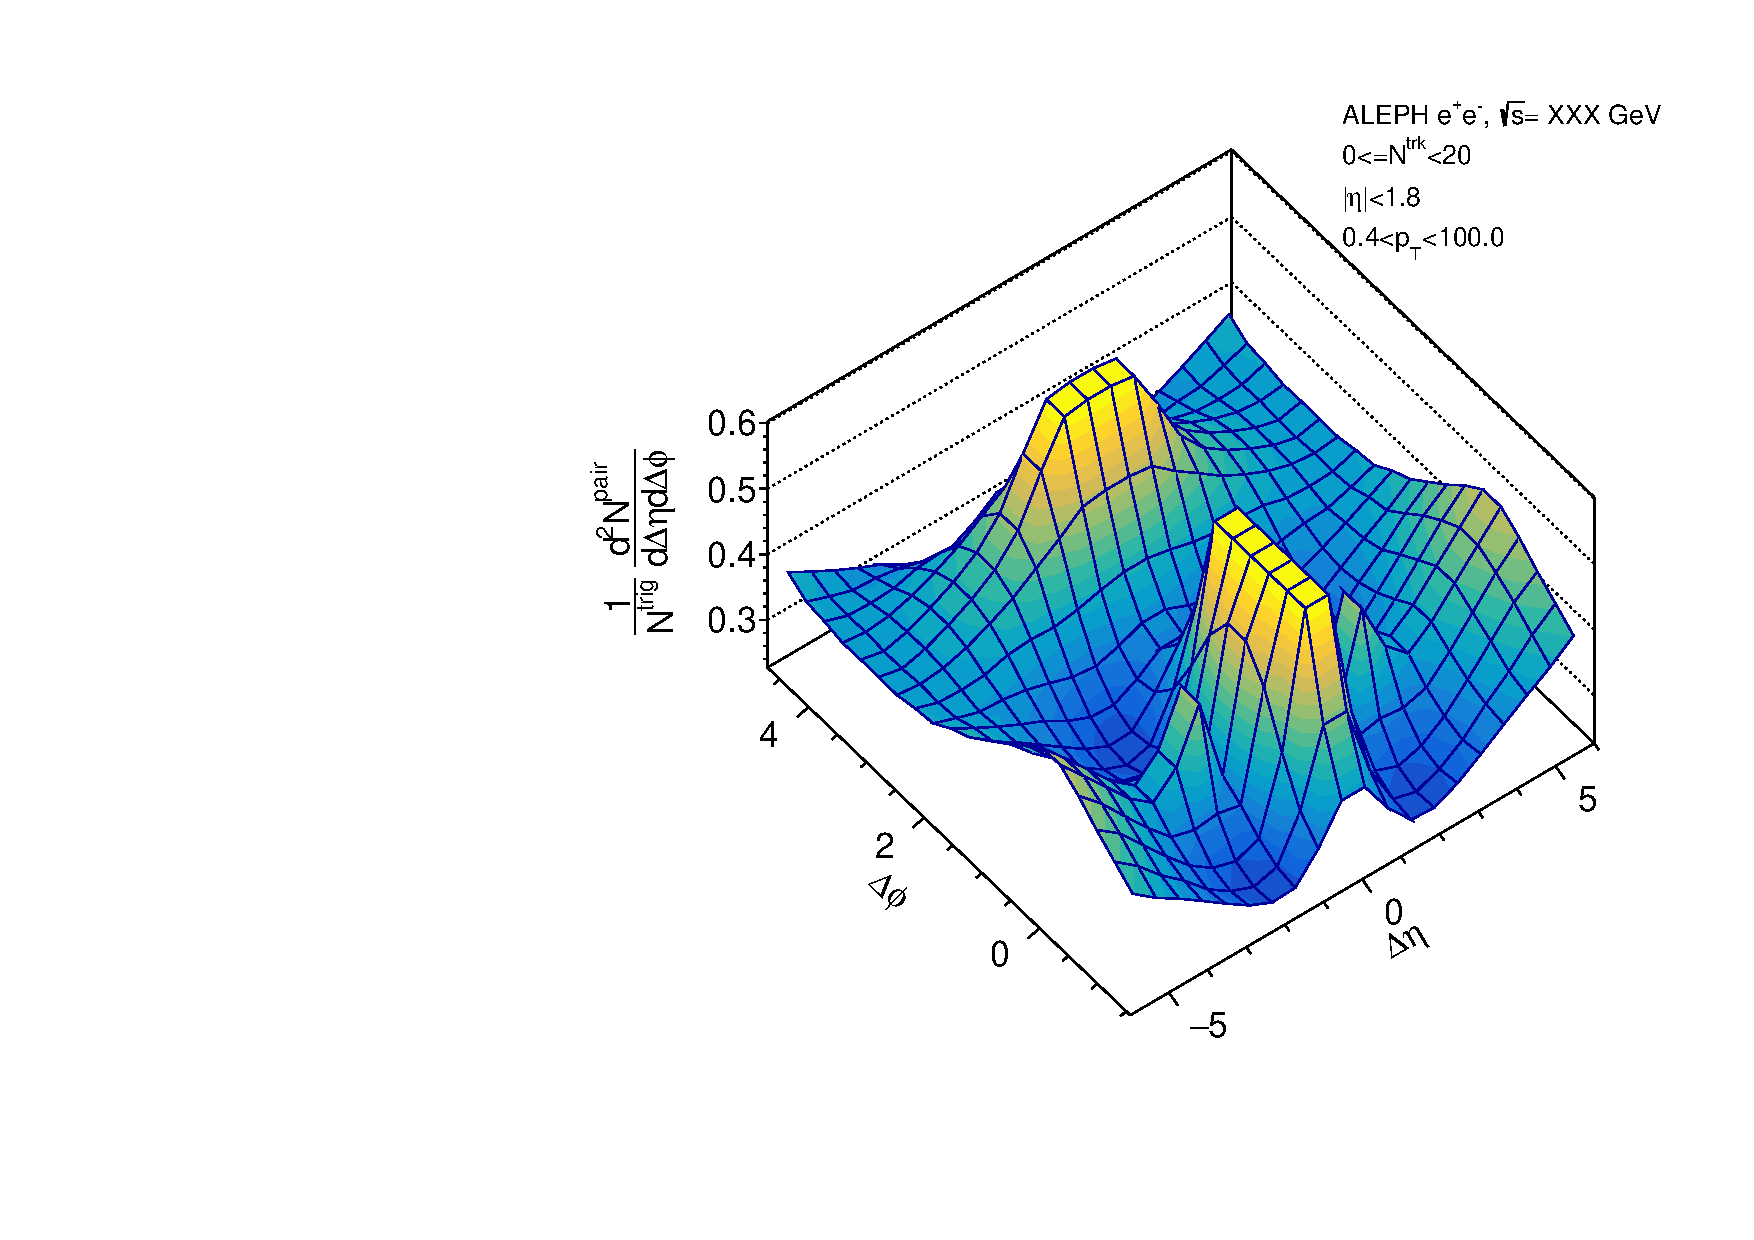
\includegraphics[width=\linewidth]{images/TwoParticleCorrelation/LEP2_THRUST/LEP2_THRUST_ratio1_0_20.pdf}
    \label{fig:LEP2 Thrust Axis, Ratio Plot, Multiplicity 0-20, Austin}
  \end{minipage}
  \hspace{0.0cm}
  \begin{minipage}[b]{0.32\linewidth}
    \centering
    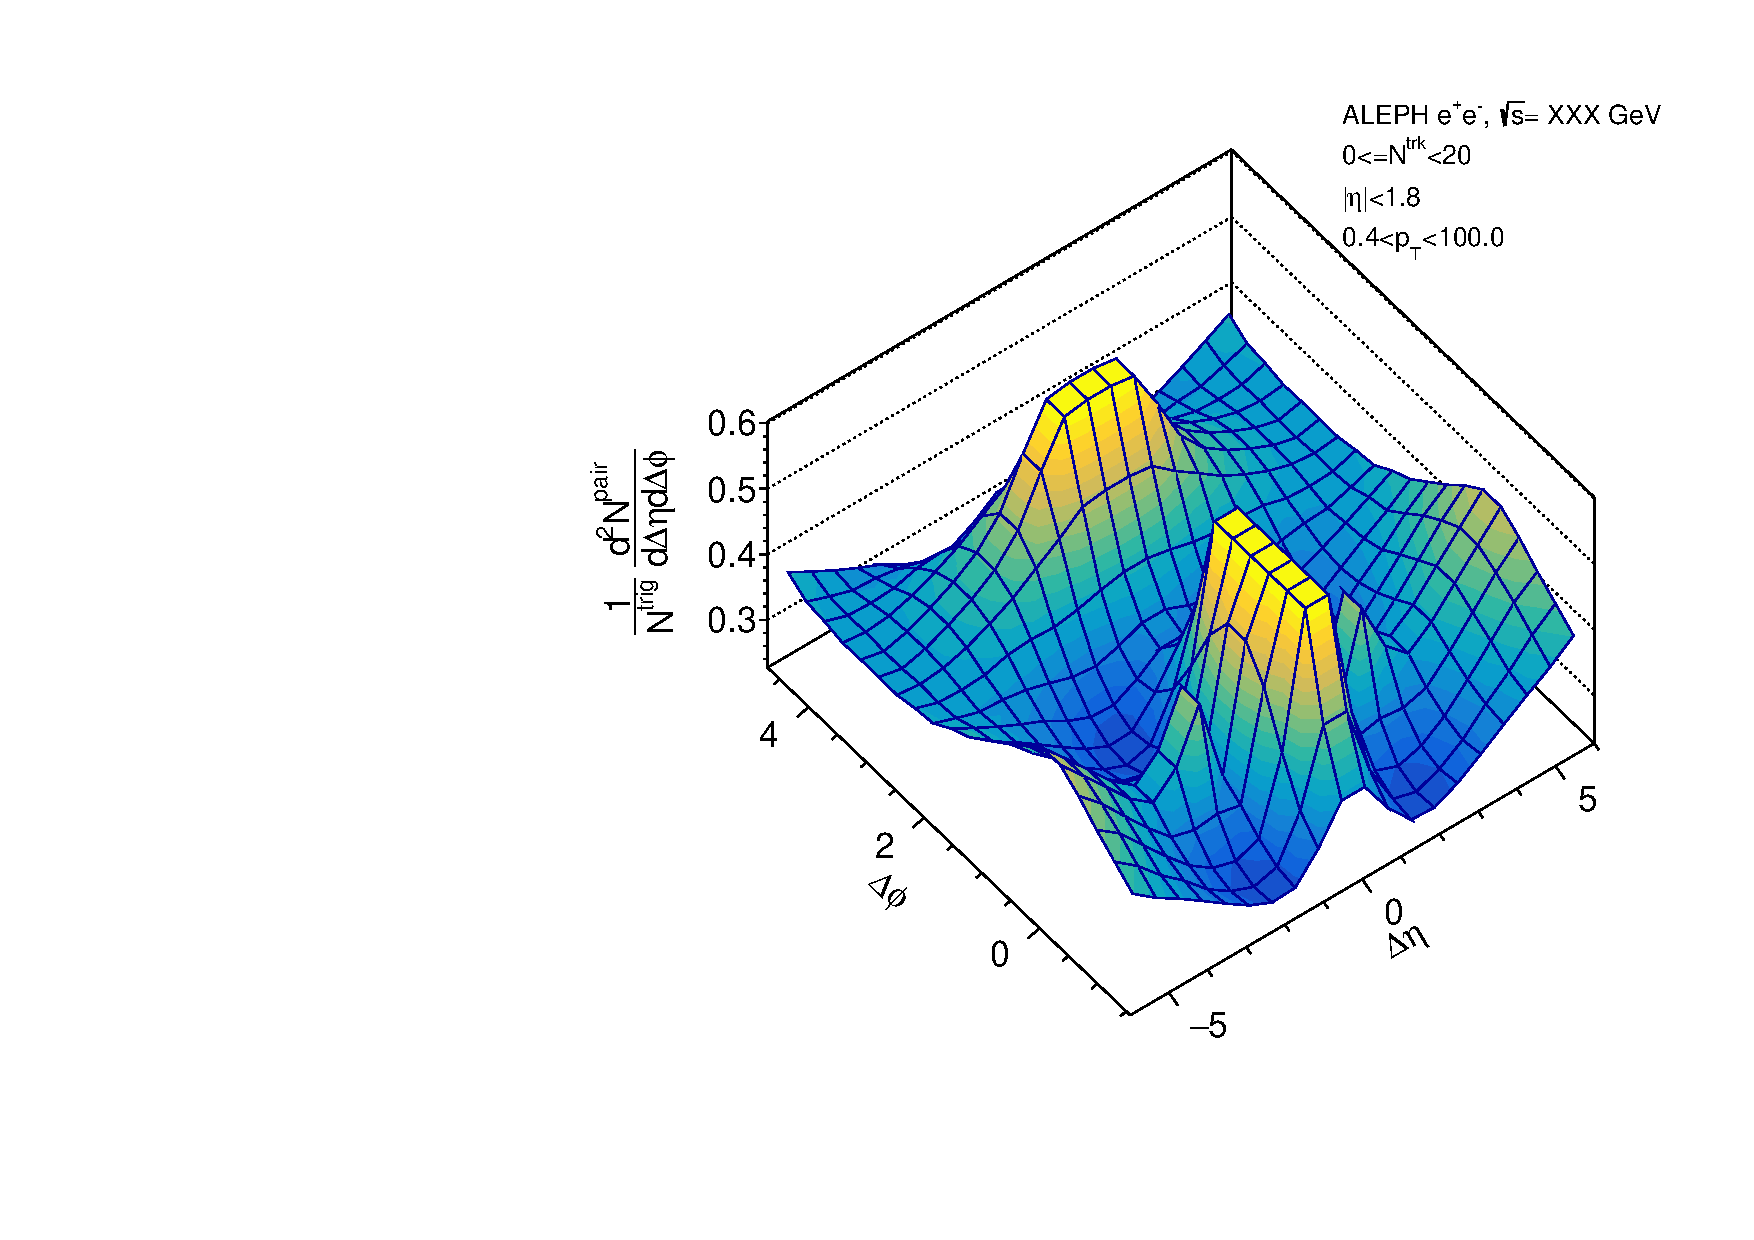
\includegraphics[width=\linewidth]{images/TwoParticleCorrelation/LEP2_THRUST/LEP2_THRUST_ratio2_0_20.pdf}
    \label{fig:LEP2 Thrust Axis, Ratio Plot, Multiplicity 0-20, Anthony}
  \end{minipage}
  \begin{minipage}[b]{0.32\linewidth}
    \centering
    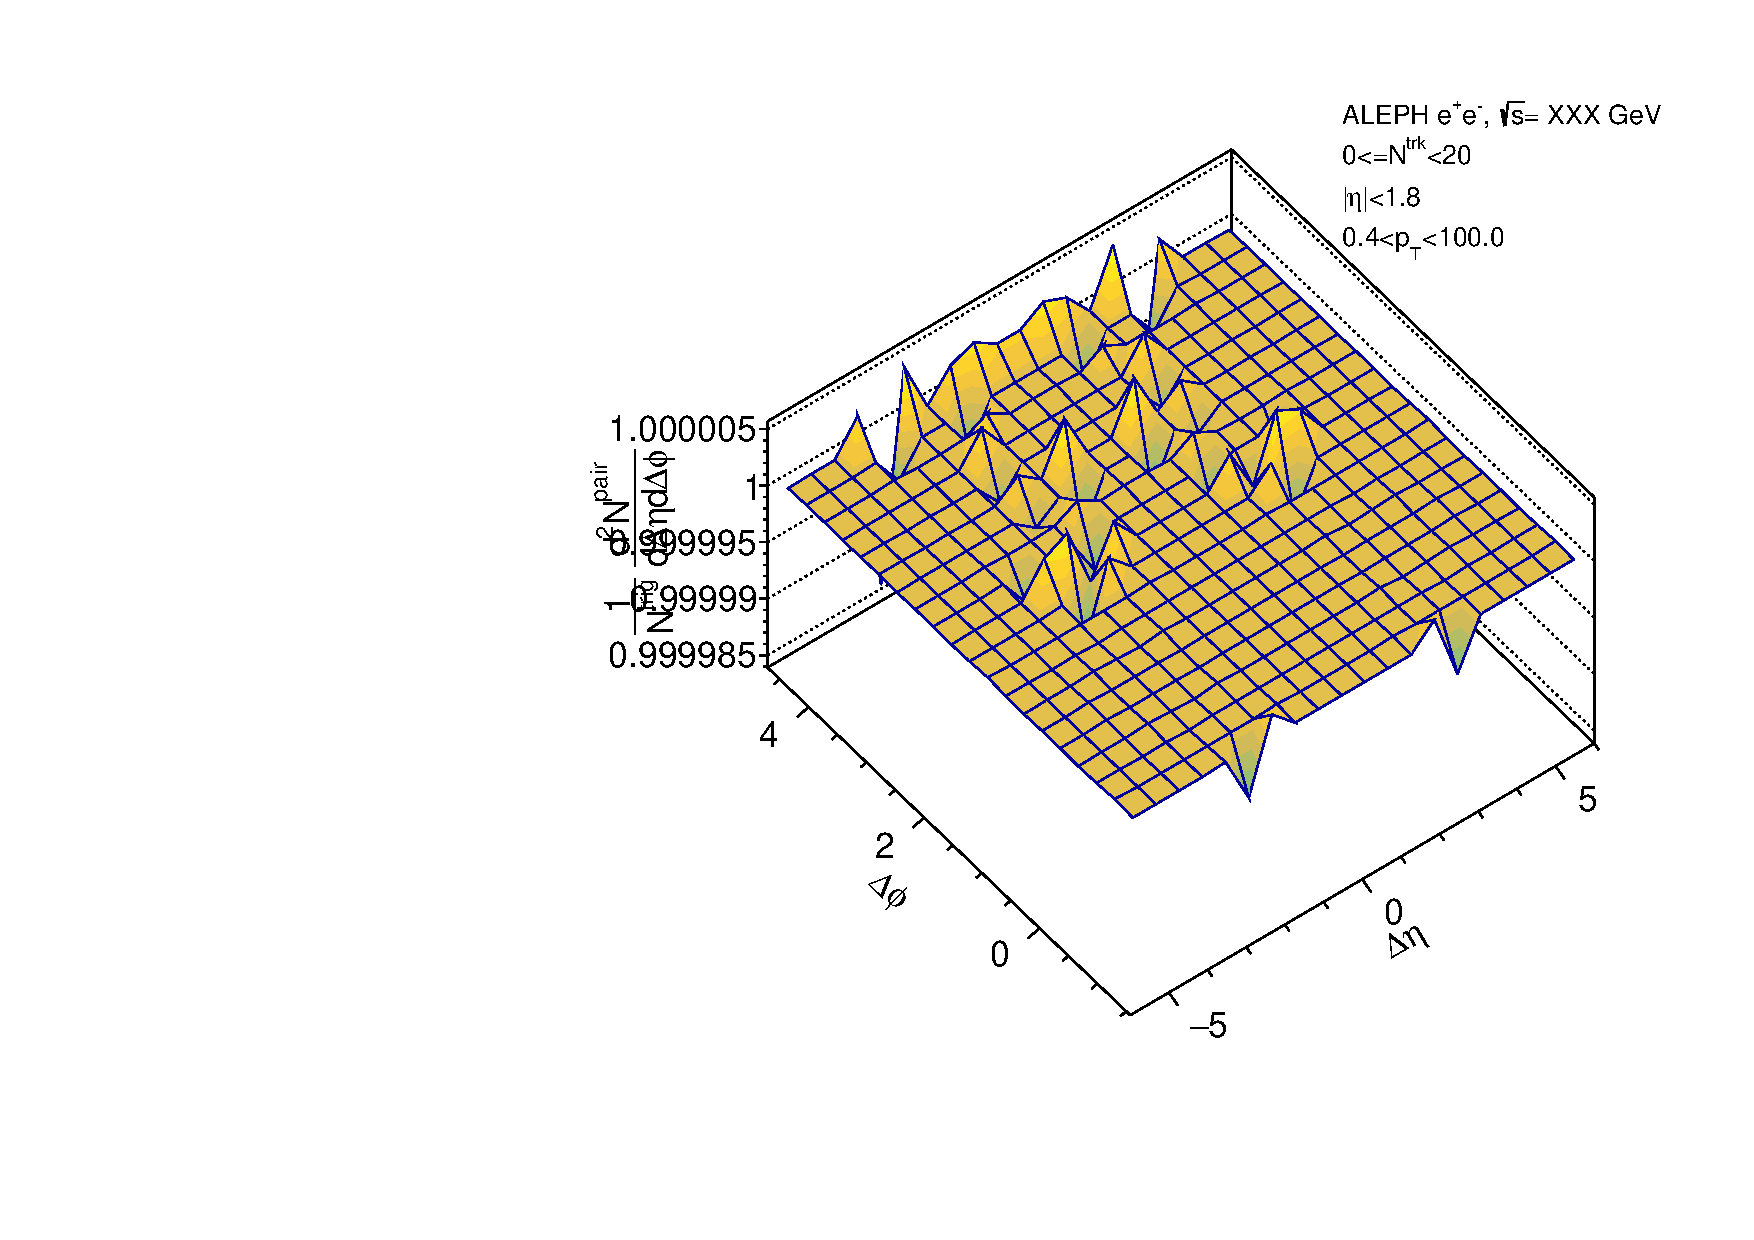
\includegraphics[width=\linewidth]{images/TwoParticleCorrelation/LEP2_THRUST/LEP2_THRUST_r_ratio_0_20.pdf}
    \label{fig:LEP2 Thrust Axis, Ratio Plot, Multiplicity 0-20, Ratio}
  \end{minipage}
\end{figure}


%%%%%%%%%%%%%%%%%%%%%%%%%%%%%%%% Multiplicity 20-30 %%%%%%%%%%%%%%%%%%%%%%%%%%%%%%%%
\begin{figure}[htbp]
  \caption{LEP2 Thrust Axis, Ratio Plot, Multiplicity 20-30 (Austin, Anthony, Ratio)}
  \begin{minipage}[b]{0.32\linewidth}
    \centering
    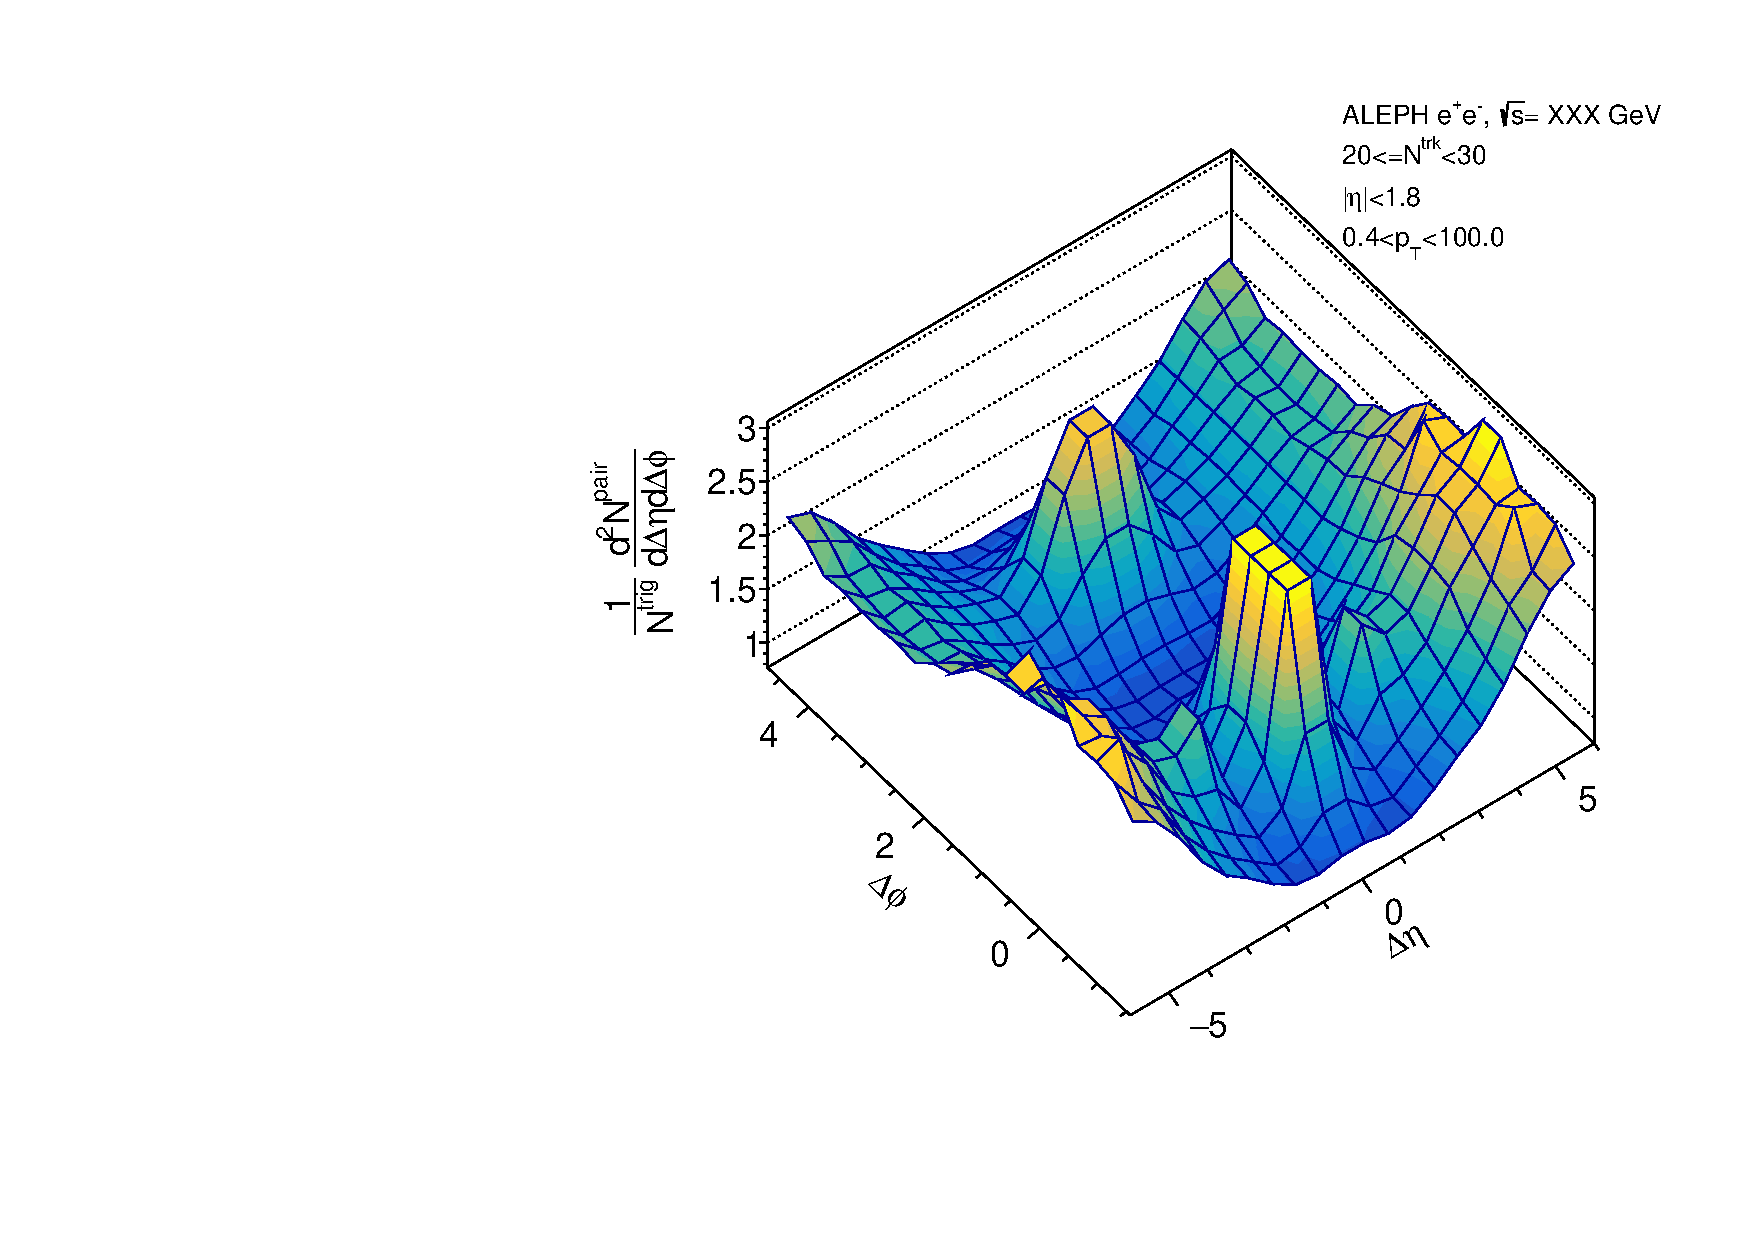
\includegraphics[width=\linewidth]{images/TwoParticleCorrelation/LEP2_THRUST/LEP2_THRUST_ratio1_20_30.pdf}
    \label{fig:LEP2 Thrust Axis, Ratio Plot, Multiplicity 20-30, Austin}
  \end{minipage}
  \hspace{0.0cm}
  \begin{minipage}[b]{0.32\linewidth}
    \centering
    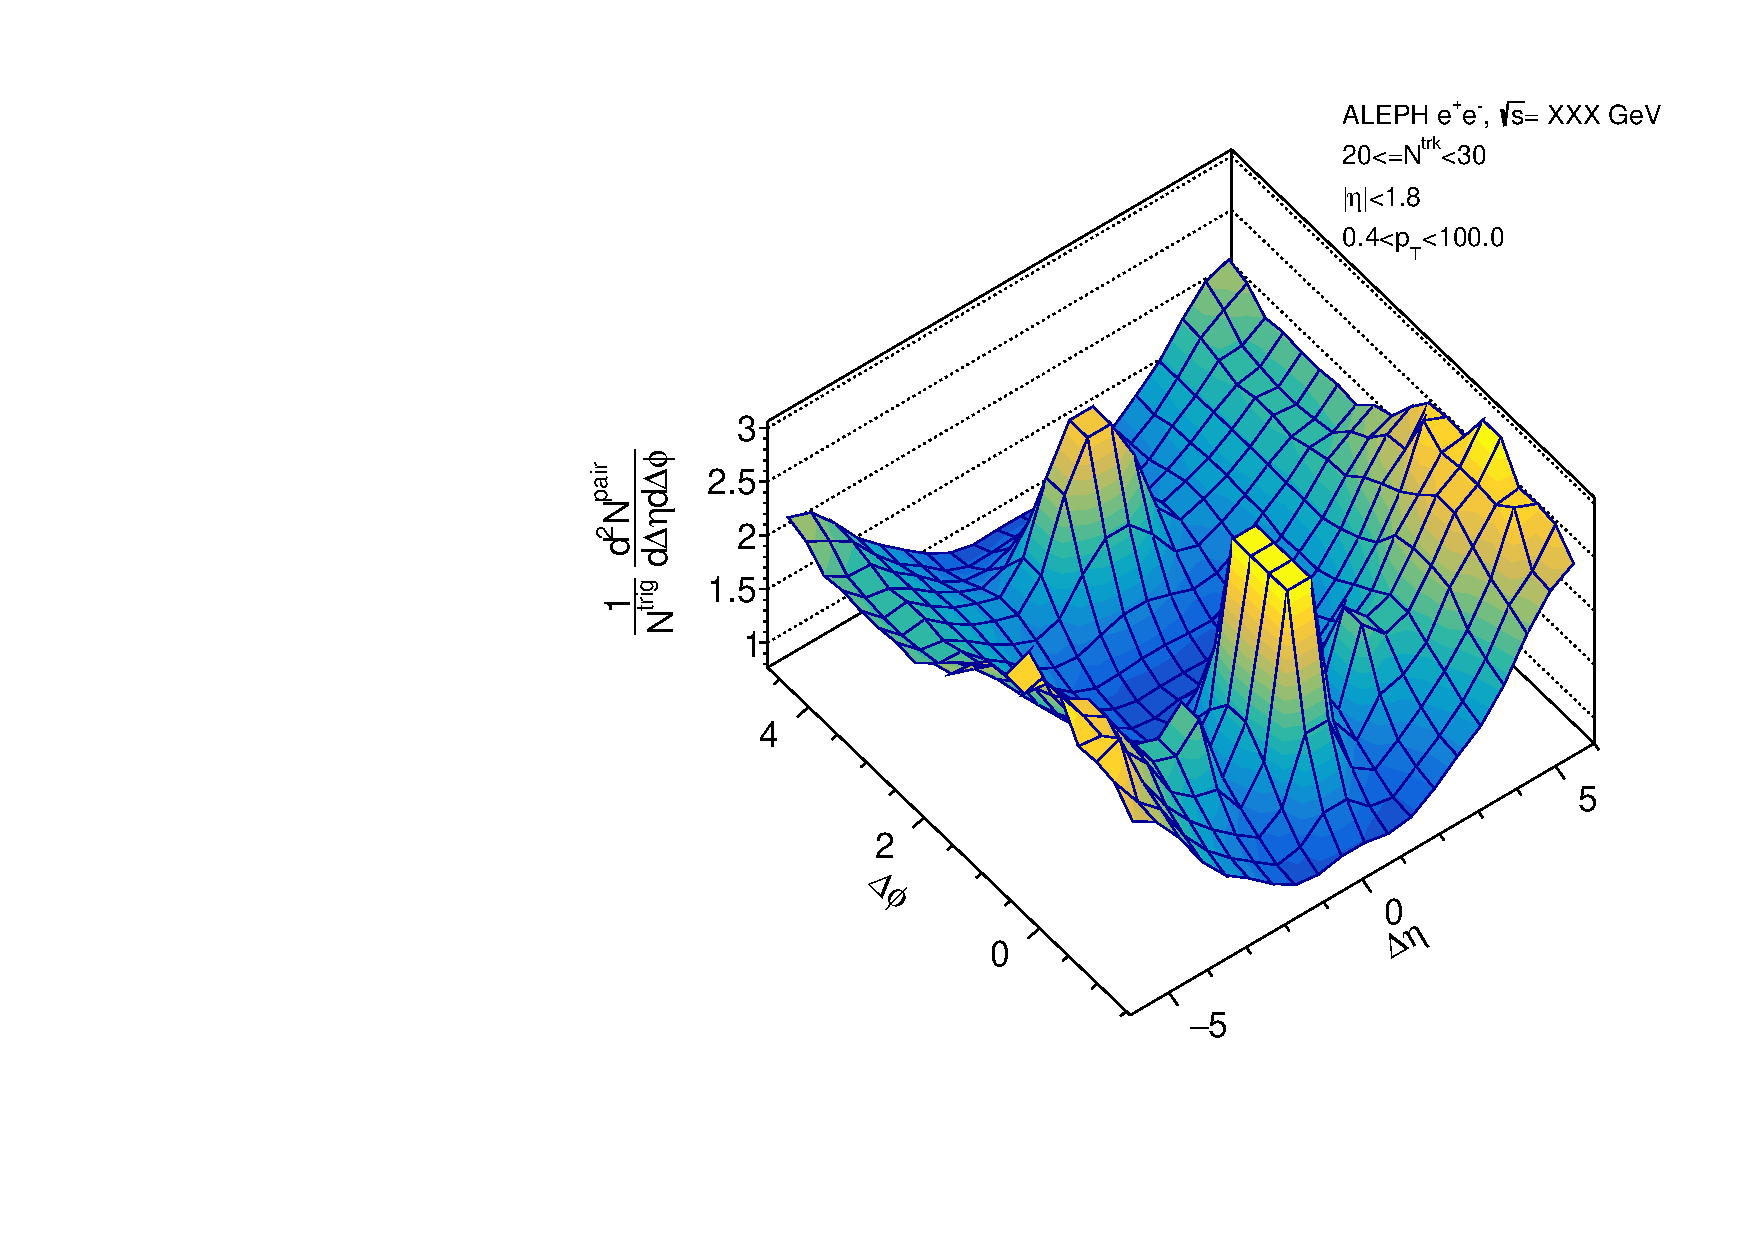
\includegraphics[width=\linewidth]{images/TwoParticleCorrelation/LEP2_THRUST/LEP2_THRUST_ratio2_20_30.pdf}
    \label{fig:LEP2 Thrust Axis, Ratio Plot, Multiplicity 20-30, Anthony}
  \end{minipage}
  \begin{minipage}[b]{0.32\linewidth}
    \centering
    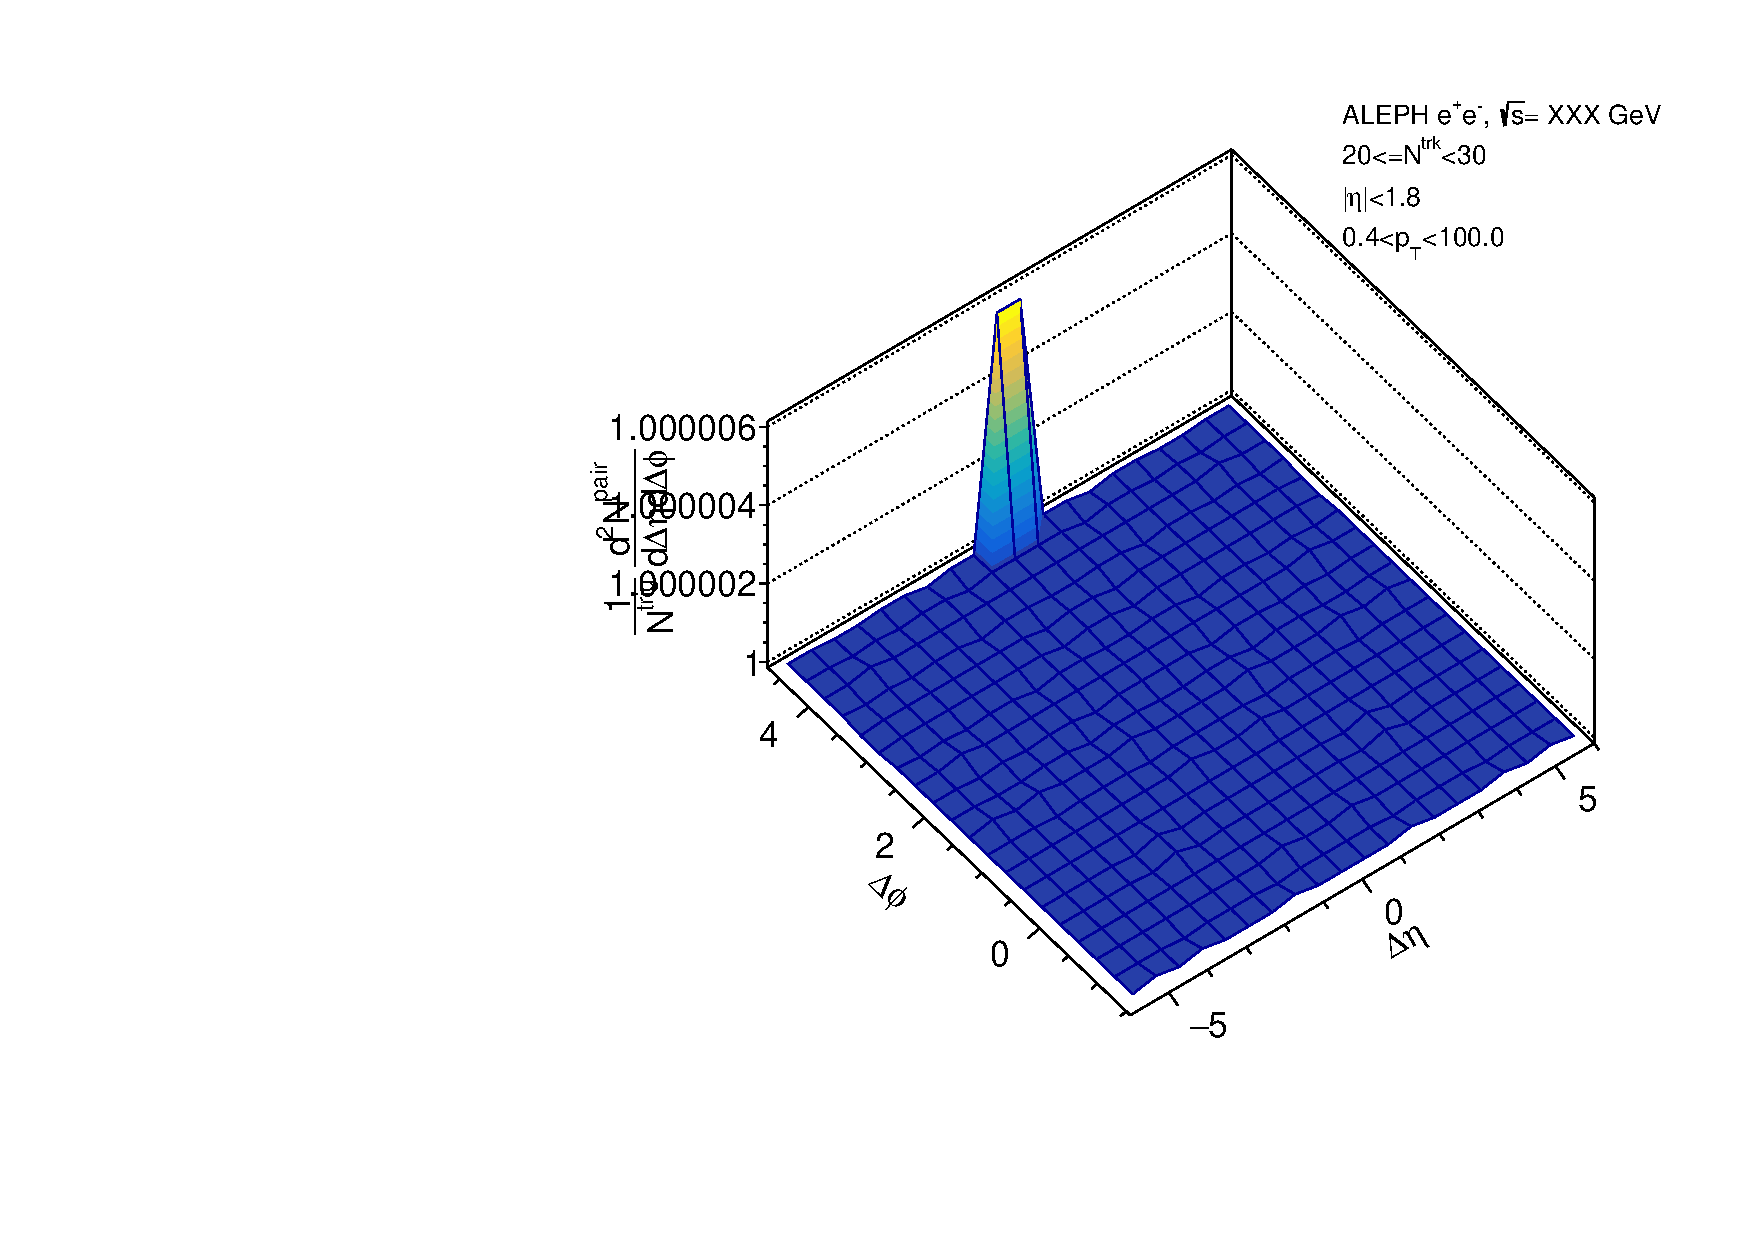
\includegraphics[width=\linewidth]{images/TwoParticleCorrelation/LEP2_THRUST/LEP2_THRUST_r_ratio_20_30.pdf}
    \label{fig:LEP2 Thrust Axis, Ratio Plot, Multiplicity 20-30, Ratio}
  \end{minipage}
\end{figure}

%%%%%%%%%%%%%%%%%%%%%%%%%%%%%%%% Multiplicity 30-999 %%%%%%%%%%%%%%%%%%%%%%%%%%%%%%%%
\begin{figure}[htbp]
  \caption{LEP2 Thrust Axis, Ratio Plot, Multiplicity 30-999 (Austin, Anthony, Ratio)}
  \begin{minipage}[b]{0.32\linewidth}
    \centering
    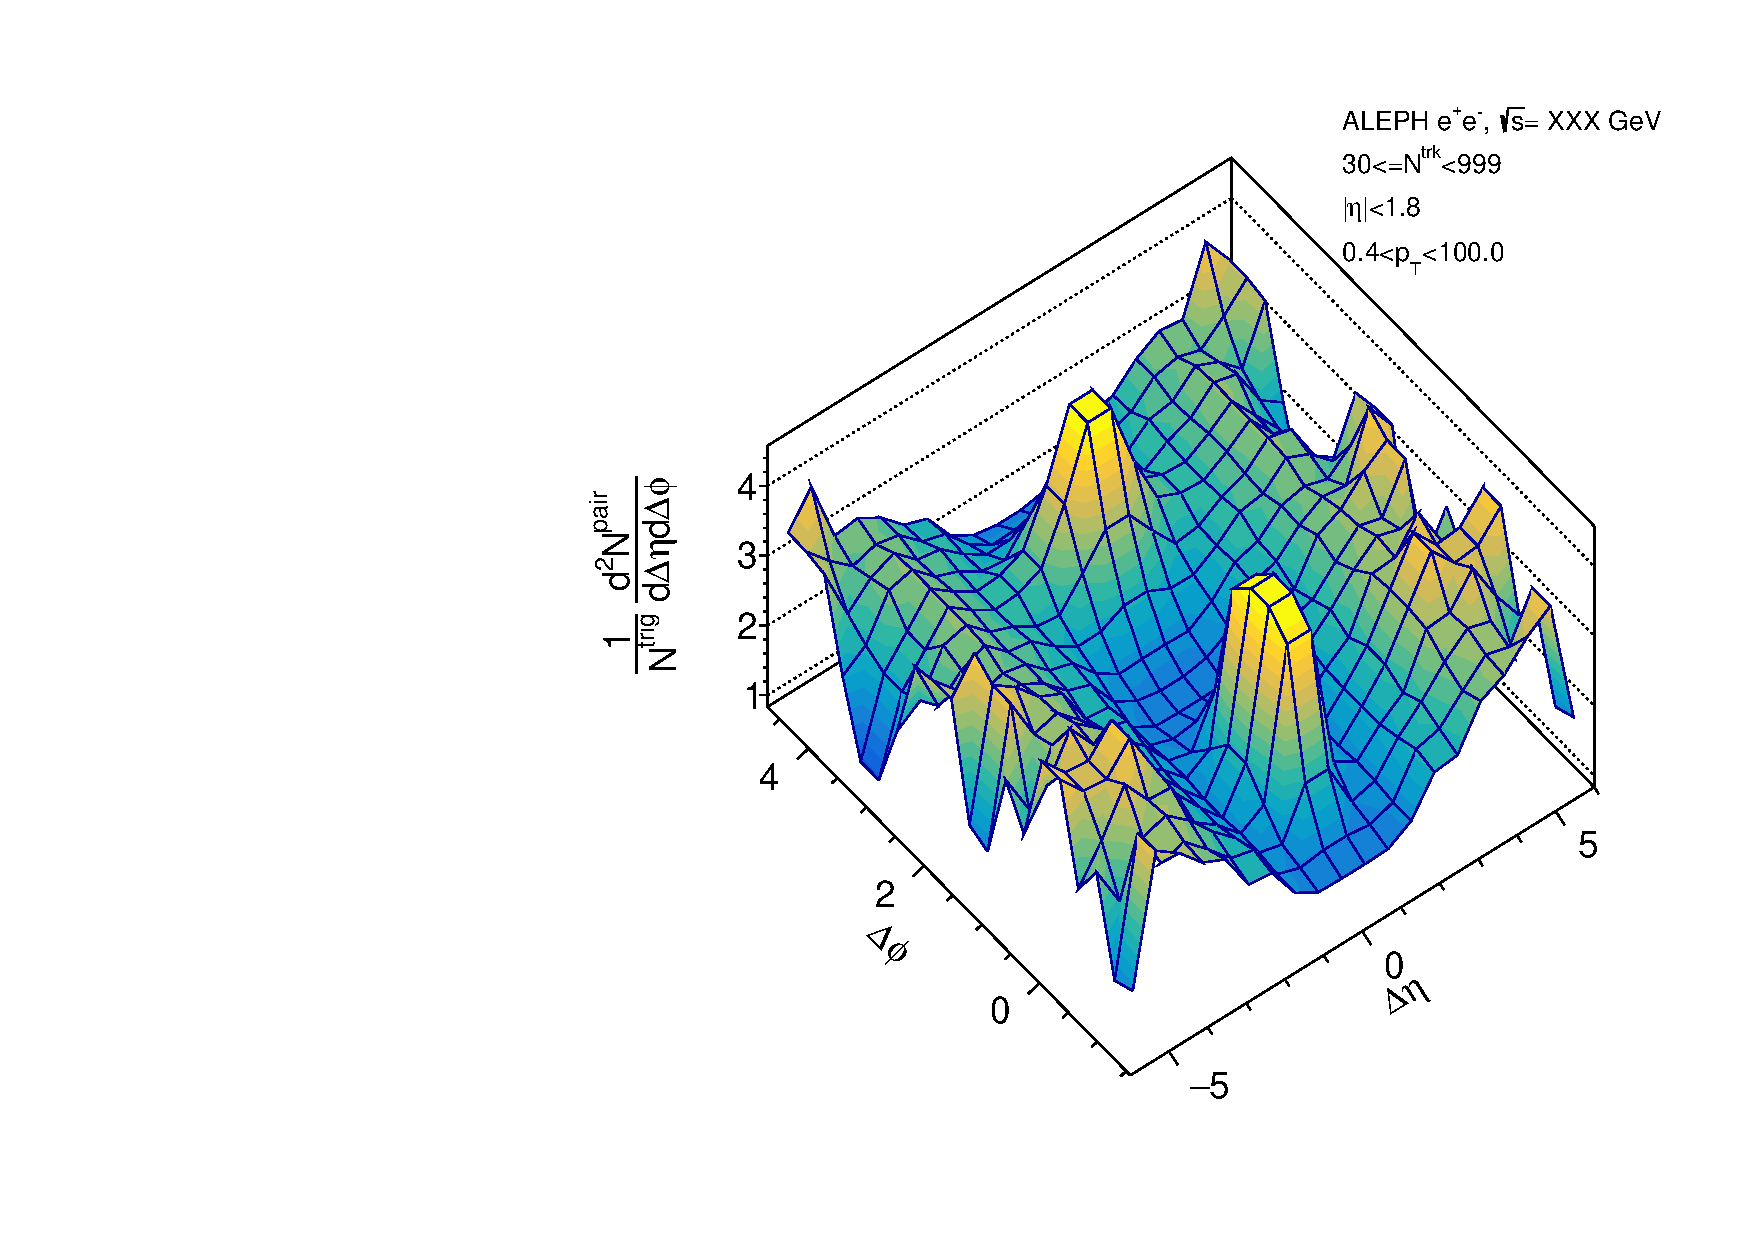
\includegraphics[width=\linewidth]{images/TwoParticleCorrelation/LEP2_THRUST/LEP2_THRUST_ratio1_30_999.pdf}
    \label{fig:LEP2 Thrust Axis, Ratio Plot, Multiplicity 30-999, Austin}
  \end{minipage}
  \hspace{0.0cm}
  \begin{minipage}[b]{0.32\linewidth}
    \centering
    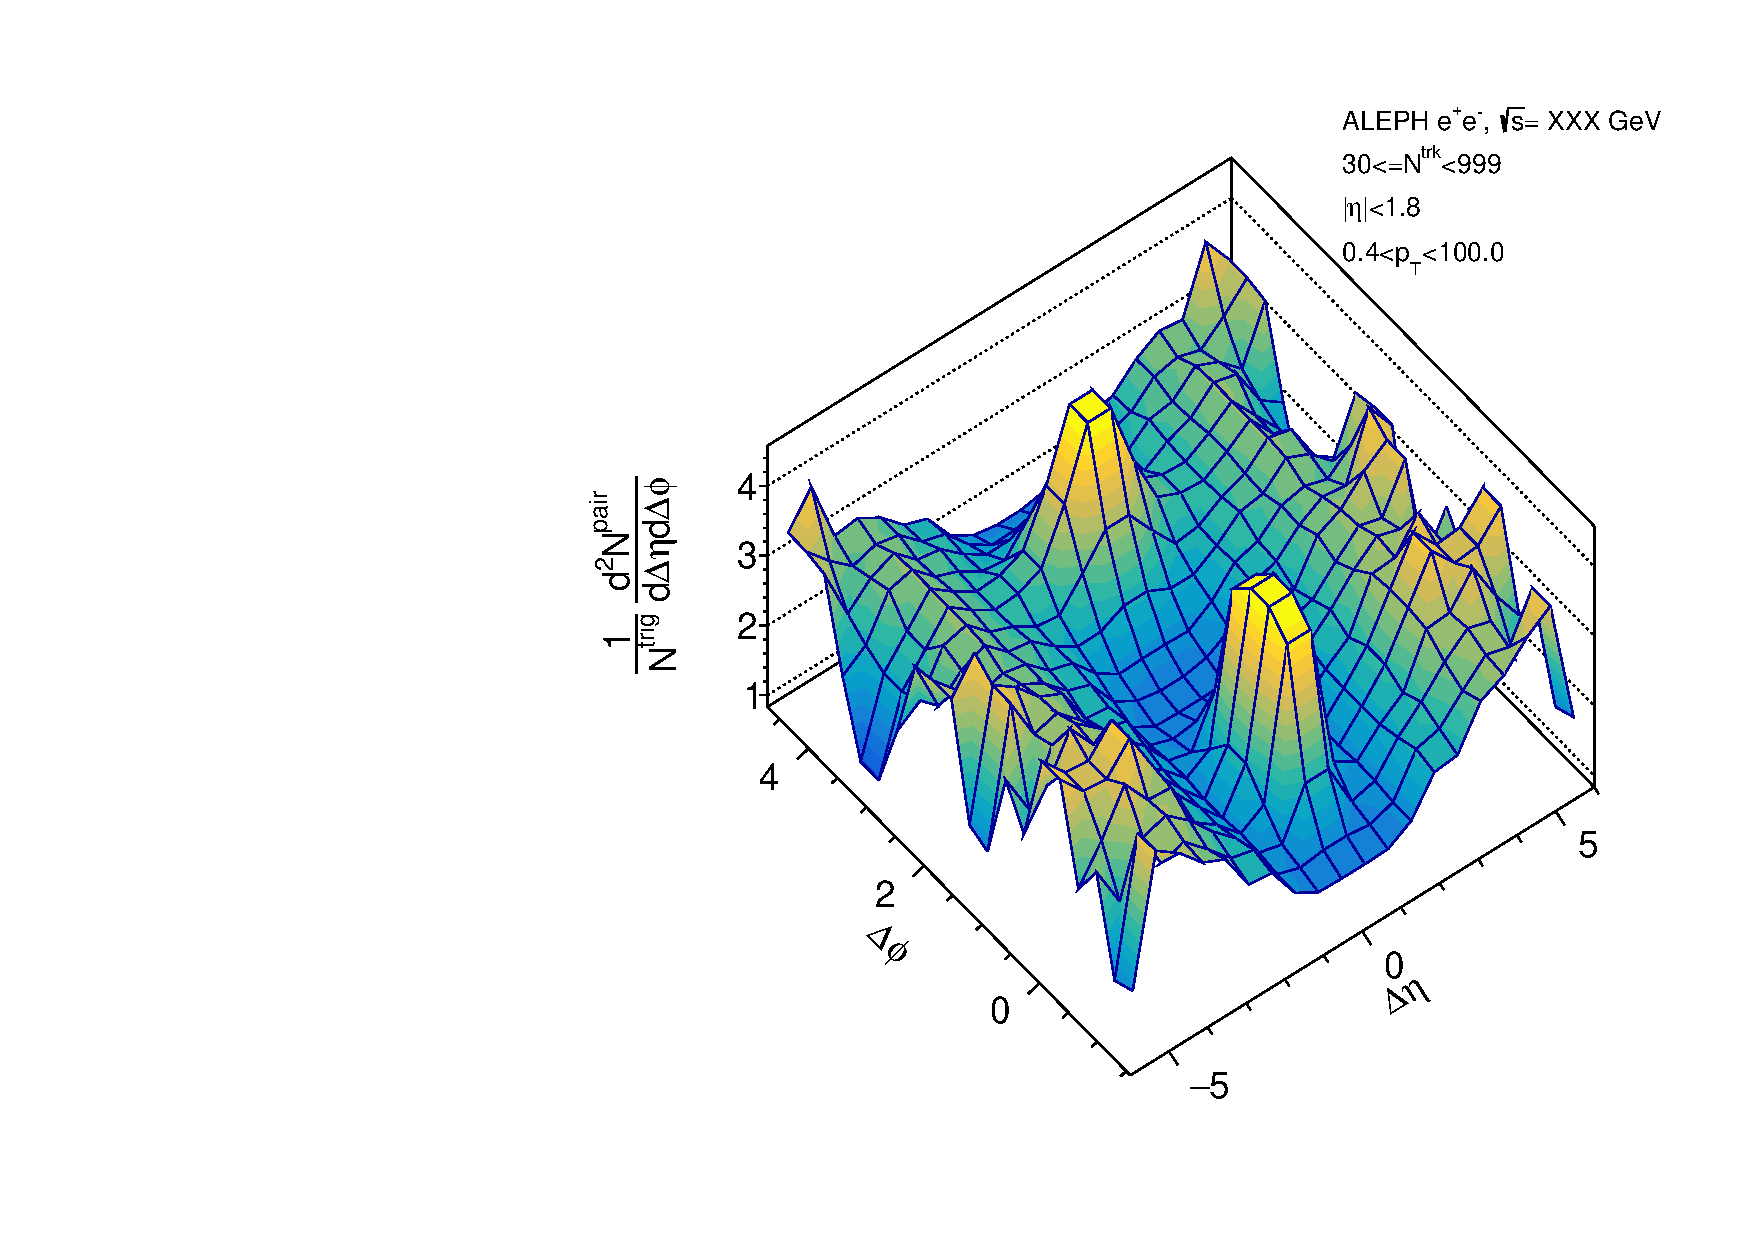
\includegraphics[width=\linewidth]{images/TwoParticleCorrelation/LEP2_THRUST/LEP2_THRUST_ratio2_30_999.pdf}
    \label{fig:LEP2 Thrust Axis, Ratio Plot, Multiplicity 30-999, Anthony}
  \end{minipage}
  \begin{minipage}[b]{0.32\linewidth}
    \centering
    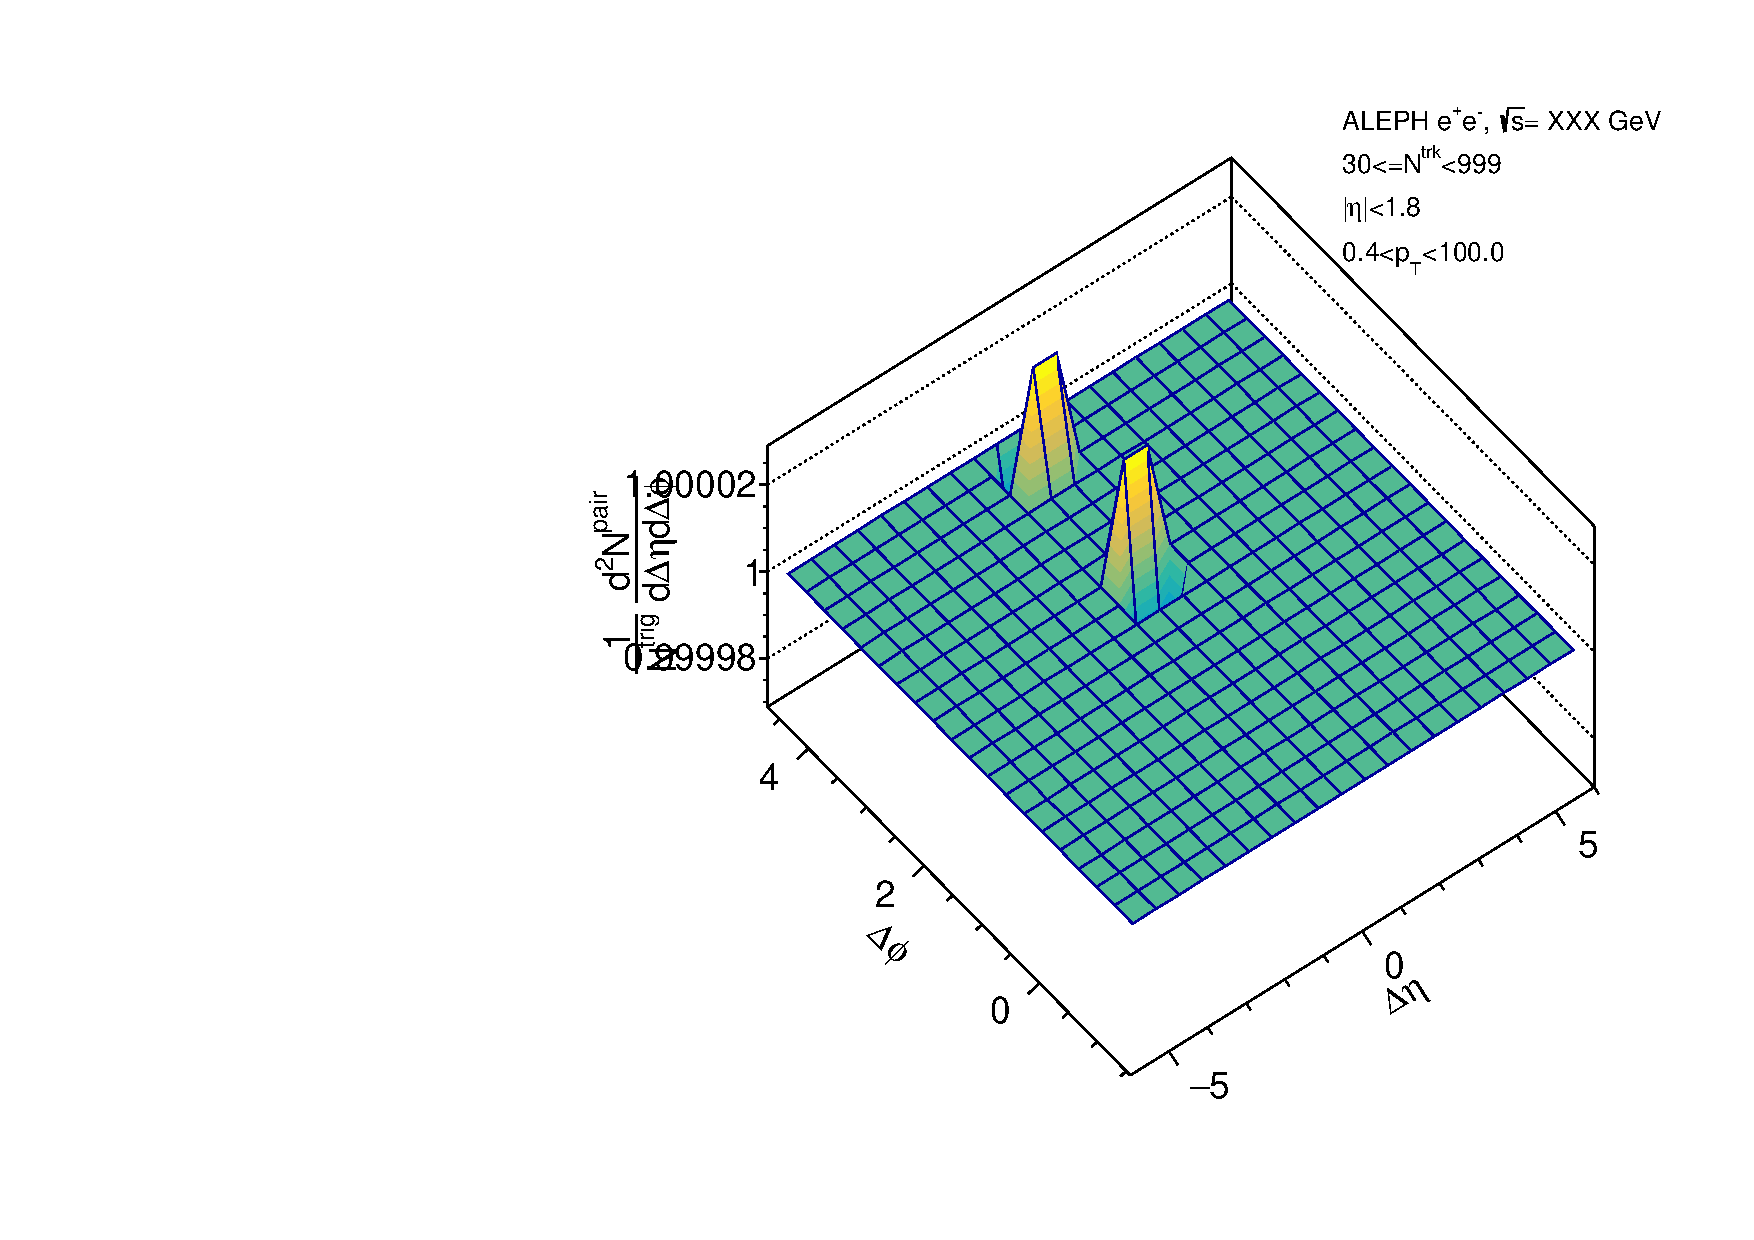
\includegraphics[width=\linewidth]{images/TwoParticleCorrelation/LEP2_THRUST/LEP2_THRUST_r_ratio_30_999.pdf}
    \label{fig:LEP2 Thrust Axis, Ratio Plot, Multiplicity 30-999, Ratio}
  \end{minipage}
\end{figure}